% Use this documentclass for the PNAS style:
% \documentclass[9pt,twocolumn,twoside,lineno]{pnas-new}

% This is for NeurIPS style:
\documentclass{article}


\makeatletter
\@ifclassloaded{pnas-new}
{
  % Use the lineno option to display guide line numbers if required.

\templatetype{pnasresearcharticle} % Choose template
% {pnasresearcharticle} = Template for a two-column research article
% {pnasmathematics} %= Template for a one-column mathematics article
% {pnasinvited} %= Template for a PNAS invited submission

%=====================================================================
%============================ our packages ===========================

\usepackage{color}
\definecolor{black}{rgb}{0,0,0}
\usepackage{amsmath}
\usepackage{amsthm}
\usepackage{tikz}
\usetikzlibrary{decorations.pathreplacing,positioning, fit, arrows.meta, shapes}
\usetikzlibrary{shapes}
\usepackage{subcaption}
\usepackage{caption}
\usepackage{pgfplots}
\usepackage{booktabs}
\usepackage{xcolor}
\usepackage{colortbl}
\usepackage{multirow}
\usepackage{hyperref}
\usepackage{float}

%=====================================================================
%============================= citations =============================


% Flexible sec/fig/tbl/def cross-refs.
\newcommand{\Secref}[1]{Section~\ref{#1}}
\newcommand{\secref}[1]{Section~\ref{#1}}
\newcommand{\dashsecref}[2]{Sections~\ref{#1}--\ref{#2}}

\newcommand{\Defref}[1]{Definition~\ref{#1}}
\newcommand{\defref}[1]{Definition~\ref{#1}}
\newcommand{\Defrefc}[2]{\Defref{#1}, clause~\ref{#2}}
\newcommand{\defrefc}[2]{\defref{#1}, clause~\ref{#2}}

\newcommand{\Figref}[1]{Figure~\ref{#1}}
\newcommand{\figref}[1]{Figure~\ref{#1}}
\newcommand{\dashfigref}[2]{Figures~\ref{#1}--\ref{#2}}
\newcommand{\Tabref}[1]{Table~\ref{#1}}
\newcommand{\tabref}[1]{Table~\ref{#1}}

\newcommand{\Appref}[1]{Appendix~\ref{#1}}
\newcommand{\appref}[1]{Appendix~\ref{#1}}

% In-text citations
\newcommand{\posscitet}[1]{\citeauthor{#1}'s~(\citeyear{#1})}
\newcommand{\sposscitet}[1]{\citeauthor{#1}'~(\citeyear{#1})}
\newcommand{\possciteauthor}[1]{\citeauthor{#1}'s}
\newcommand{\spossciteauthor}[1]{\citeauthor{#1}'}
\newcommand{\pgposscitet}[2]{\citeauthor{#1}'s~(\citeyear{#1}:~#2)}
\newcommand{\secposscitet}[2]{\citeauthor{#1}'s~(\citeyear{#1}:~$\S$#2)}
\newcommand{\pgcitealt}[2]{\citealt{#1}:~#2}
\newcommand{\seccitealt}[2]{\citealt{#1}:~$\S$#2}
\newcommand{\pgcitep}[2]{(\citealt{#1}:~#2)}
\newcommand{\seccitep}[2]{(\citealt{#1}:~$\S$#2)}
\newcommand{\pgcitet}[2]{\citeauthor{#1}~(\citeyear{#1}:~#2)}
\newcommand{\seccitet}[2]{\citeauthor{#1}~(\citeyear{#1}:~$\S$#2)}

% Examples:
\newcommand{\eg}[1]{(\ref{#1})}
\newcommand{\dasheg}[2]{\eg{#1}--\eg{#2}}
\newcommand{\subeg}[2]{(\ref{#1}\ref{#2})}
\newcommand{\dblsubeg}[3]{(\ref{#1}\ref{#2},~\ref{#3})}
\newcommand{\dashsubeg}[3]{(\ref{#1}\ref{#2}--\ref{#3})}

%=====================================================================
%========================= font manipulation =========================

\newcommand{\word}[1]{\emph{#1}}
\newcommand{\tech}[1]{\emph{#1}}
\newcommand{\highlight}[1]{\textbf{#1}}

\newcommand{\blue}[1]{{\color{blue}#1}}

\definecolor{ourgreen}{HTML}{4D8951}
\definecolor{darkblue}{HTML}{0499CC}
\definecolor{darkred}{HTML}{8B0000}
\definecolor{superlightgray}{HTML}{B8B8B8}

\newcommand{\poscell}[1]{\fcolorbox{white}{ourgreen}{#1}}
\newcommand{\negcell}[1]{\fcolorbox{white}{superlightgray}{#1}}


% \newcommand{\update}[1]{{\color{darkblue}#1}}
% \newcommand{\updatea}[1]{{\color{darkred}#1}}
% \newcommand{\updateb}[1]{{\color{ourgreen}#1}}

\newcommand{\update}[1]{#1}
\newcommand{\updatea}[1]{#1}
\newcommand{\updateb}[1]{#1}

%=====================================================================
%================================ math ===============================

\newcommand{\softmax}{\mathbf{softmax}}
\DeclareMathOperator{\ReLU}{ReLU}
\newcommand{\identity}{\mathbb{I}}
\newcommand{\LSTM}{\textbf{LSTM}}
\newcommand{\wupdate}{\mathrel{{+}{=}}}



\newcommand{\inputcolor}{black!20}
\newcommand{\outputcolor}{red!40}
\newcommand{\hiddencolor}{blue!40}
\newcommand{\hiddencolortwo}{orange!40}
\newcommand{\colorlabel}{green!40}
\newcommand{\compare}{\emph{Euclidean}}

\title{% Generalized relational reasoning using neural networks with non-featural representations
Relational reasoning and generalization using non-symbolic neural networks}

% Use letters for affiliations, numbers to show equal authorship (if applicable) and to indicate the corresponding author
\author[a,1]{Atticus Geiger}
\author[b]{Alexandra Carstensen}
\author[b]{Michael C.~Frank}
\author[a]{Christopher Potts}

\affil[a]{Department of Linguistics, Stanford University}
\affil[b]{Department of Psychology, Stanford University}

% Please give the surname of the lead author for the running footer
\leadauthor{Geiger}

% Please add here a significance statement to explain the relevance of your work
\significancestatement{Authors must submit a 120-word maximum statement about the significance of their research paper written at a level understandable to an undergraduate educated scientist outside their field of speciality. The primary goal of the Significance Statement is to explain the relevance of the work in broad context to a broad readership. The Significance Statement appears in the paper itself and is required for all research papers.}

% Please include corresponding author, author contribution and author declaration information
\authorcontributions{Please provide details of author contributions here.}
\authordeclaration{Please declare any conflict of interest here.}
% \equalauthors{\textsuperscript{1}A.O.(Author One) and A.T. (Author Two) contributed equally to this work (remove if not applicable).}
\correspondingauthor{\textsuperscript{1}To whom correspondence should be addressed. E-mail: ageiger@stanford.edu}

% Keywords are not mandatory, but authors are strongly encouraged to provide them. If provided, please include two to five keywords, separated by the pipe symbol, e.g:
\keywords{Keyword 1 $|$ Keyword 2 $|$ Keyword 3 $|$ ...}

\begin{abstract}
  Humans have a remarkable capacity to reason about abstract relational structures, an ability that may support some of the most impressive, human-unique cognitive feats. Because equality (or identity) is a simple and ubiquitous relational operator, equality reasoning has been a key case study for the broader question of abstract relational reasoning. This paper revisits the question of whether equality can be learned by neural networks that do not encode explicit symbolic structure. Earlier work arrived at a negative answer to this question, but that result holds only for a particular class of hand-crafted feature representations. In our experiments, we assess out-of-sample generalization of equality using both arbitrary representations and representations that have been pretrained on separate tasks to imbue them with abstract structure. In this setting, even simple neural networks are able to learn basic equality with relatively little training data. In a second case study, we show that sequential equality problems (learning ABA sequences) can be solved with only positive training instances. Finally, we consider a more complex, hierarchical equality problem, but this requires vastly more data. However, using a pretrained equality network as a modular component of this larger task leads to good performance with no task-specific training. Overall, these findings indicate that neural models are able to solve equality-based reasoning tasks, suggesting that essential aspects of symbolic reasoning can emerge from data-driven, non-symbolic learning processes.
\end{abstract}

\dates{This manuscript was compiled on \today}
\doi{\url{www.pnas.org/cgi/doi/10.1073/pnas.XXXXXXXXXX}}

\begin{document}

\maketitle
\thispagestyle{firststyle}
\ifthenelse{\boolean{shortarticle}}{\ifthenelse{\boolean{singlecolumn}}{\abscontentformatted}{\abscontent}}{}

% If your first paragraph (i.e. with the \dropcap) contains a list environment (quote, quotation, theorem, definition, enumerate, itemize...), the line after the list may have some extra indentation. If this is the case, add \parshape=0 to the end of the list environment.

% \section{Introduction}\label{sec:introduction}
  \newcommand{\papermode}{pnas}
}
{
  % if you need to pass options to natbib, use, e.g.:
%     \PassOptionsToPackage{numbers, compress}{natbib}
% before loading neurips_2020

% ready for submission
% \usepackage{neurips_2020}

% to compile a preprint version, e.g., for submission to arXiv, add add the
% [preprint] option:
\usepackage[preprint]{neurips_2020}

% to compile a camera-ready version, add the [final] option, e.g.:
%     \usepackage[final]{neurips_2020}

% to avoid loading the natbib package, add option nonatbib:
%     \usepackage[nonatbib]{neurips_2020}

\usepackage[utf8]{inputenc} % allow utf-8 input
\usepackage[T1]{fontenc}    % use 8-bit T1 fonts0
\usepackage{url}            % simple URL typesetting
\usepackage{booktabs}       % professional-quality tables
\usepackage{amsfonts}       % blackboard math symbols
\usepackage{nicefrac}       % compact symbols for 1/2, etc.
\usepackage{microtype}      % microtypography

\usepackage[colorlinks, linkcolor=black, urlcolor=black, citecolor=black]{hyperref}

%=====================================================================
%============================ our packages ===========================

\usepackage{color}
\definecolor{black}{rgb}{0,0,0}
\usepackage{amsmath}
\usepackage{amsthm}
\usepackage{tikz}
\usetikzlibrary{decorations.pathreplacing,positioning, fit, arrows.meta, shapes}
\usetikzlibrary{shapes}
\usepackage{subcaption}
\usepackage{caption}
\usepackage{pgfplots}
\usepackage{booktabs}
\usepackage{xcolor}
\usepackage{colortbl}
\usepackage{multirow}
\usepackage{hyperref}
\usepackage{float}

%=====================================================================
%============================= citations =============================


% Flexible sec/fig/tbl/def cross-refs.
\newcommand{\Secref}[1]{Section~\ref{#1}}
\newcommand{\secref}[1]{Section~\ref{#1}}
\newcommand{\dashsecref}[2]{Sections~\ref{#1}--\ref{#2}}

\newcommand{\Defref}[1]{Definition~\ref{#1}}
\newcommand{\defref}[1]{Definition~\ref{#1}}
\newcommand{\Defrefc}[2]{\Defref{#1}, clause~\ref{#2}}
\newcommand{\defrefc}[2]{\defref{#1}, clause~\ref{#2}}

\newcommand{\Figref}[1]{Figure~\ref{#1}}
\newcommand{\figref}[1]{Figure~\ref{#1}}
\newcommand{\dashfigref}[2]{Figures~\ref{#1}--\ref{#2}}
\newcommand{\Tabref}[1]{Table~\ref{#1}}
\newcommand{\tabref}[1]{Table~\ref{#1}}

\newcommand{\Appref}[1]{Appendix~\ref{#1}}
\newcommand{\appref}[1]{Appendix~\ref{#1}}

% In-text citations
\newcommand{\posscitet}[1]{\citeauthor{#1}'s~(\citeyear{#1})}
\newcommand{\sposscitet}[1]{\citeauthor{#1}'~(\citeyear{#1})}
\newcommand{\possciteauthor}[1]{\citeauthor{#1}'s}
\newcommand{\spossciteauthor}[1]{\citeauthor{#1}'}
\newcommand{\pgposscitet}[2]{\citeauthor{#1}'s~(\citeyear{#1}:~#2)}
\newcommand{\secposscitet}[2]{\citeauthor{#1}'s~(\citeyear{#1}:~$\S$#2)}
\newcommand{\pgcitealt}[2]{\citealt{#1}:~#2}
\newcommand{\seccitealt}[2]{\citealt{#1}:~$\S$#2}
\newcommand{\pgcitep}[2]{(\citealt{#1}:~#2)}
\newcommand{\seccitep}[2]{(\citealt{#1}:~$\S$#2)}
\newcommand{\pgcitet}[2]{\citeauthor{#1}~(\citeyear{#1}:~#2)}
\newcommand{\seccitet}[2]{\citeauthor{#1}~(\citeyear{#1}:~$\S$#2)}

% Examples:
\newcommand{\eg}[1]{(\ref{#1})}
\newcommand{\dasheg}[2]{\eg{#1}--\eg{#2}}
\newcommand{\subeg}[2]{(\ref{#1}\ref{#2})}
\newcommand{\dblsubeg}[3]{(\ref{#1}\ref{#2},~\ref{#3})}
\newcommand{\dashsubeg}[3]{(\ref{#1}\ref{#2}--\ref{#3})}

%=====================================================================
%========================= font manipulation =========================

\newcommand{\word}[1]{\emph{#1}}
\newcommand{\tech}[1]{\emph{#1}}
\newcommand{\highlight}[1]{\textbf{#1}}

\newcommand{\blue}[1]{{\color{blue}#1}}

\definecolor{ourgreen}{HTML}{4D8951}
\definecolor{darkblue}{HTML}{0499CC}
\definecolor{darkred}{HTML}{8B0000}
\definecolor{superlightgray}{HTML}{B8B8B8}

\newcommand{\poscell}[1]{\fcolorbox{white}{ourgreen}{#1}}
\newcommand{\negcell}[1]{\fcolorbox{white}{superlightgray}{#1}}


% \newcommand{\update}[1]{{\color{darkblue}#1}}
% \newcommand{\updatea}[1]{{\color{darkred}#1}}
% \newcommand{\updateb}[1]{{\color{ourgreen}#1}}

\newcommand{\update}[1]{#1}
\newcommand{\updatea}[1]{#1}
\newcommand{\updateb}[1]{#1}

%=====================================================================
%================================ math ===============================

\newcommand{\softmax}{\mathbf{softmax}}
\DeclareMathOperator{\ReLU}{ReLU}
\newcommand{\identity}{\mathbb{I}}
\newcommand{\LSTM}{\textbf{LSTM}}
\newcommand{\wupdate}{\mathrel{{+}{=}}}



\newcommand{\inputcolor}{black!20}
\newcommand{\outputcolor}{red!40}
\newcommand{\hiddencolor}{blue!40}
\newcommand{\hiddencolortwo}{orange!40}
\newcommand{\colorlabel}{green!40}
\newcommand{\compare}{\emph{Euclidean}}


\newcommand{\dropcap}[1]{#1}

%=====================================================================
%=====================================================================


\title{% Generalized relational reasoning using neural networks with non-featural representations
Relational reasoning and generalization using non-symbolic neural networks}

% The \author macro works with any number of authors. There are two commands
% used to separate the names and addresses of multiple authors: \And and \AND.
%
% Using \And between authors leaves it to LaTeX to determine where to break the
% lines. Using \AND forces a line break at that point. So, if LaTeX puts 3 of 4
% authors names on the first line, and the last on the second line, try using
% \AND instead of \And before the third author name.

\author{%
  Atticus Geiger \\
  Department of Linguistics\\
  Stanford University \\
  \And
  Alexandra Carstensen \\
  Department of Psychology \\
  Stanford University \\
  \AND
  Michael C.~Frank \\
  Department of Psychology \\
  Stanford University \\
  \And
  Christopher Potts \\
  Department of Linguistics\\
  Stanford University
}


\begin{document}

\maketitle

\begin{abstract}
  Humans have a remarkable capacity to reason about abstract relational structures, an ability that may support some of the most impressive, human-unique cognitive feats. Because equality (or identity) is a simple and ubiquitous relational operator, equality reasoning has been a key case study for the broader question of abstract relational reasoning. This paper revisits the question of whether equality can be learned by neural networks that do not encode explicit symbolic structure. Earlier work arrived at a negative answer to this question, but that result holds only for a particular class of hand-crafted feature representations. In our experiments, we assess out-of-sample generalization of equality using both arbitrary representations and representations that have been pretrained on separate tasks to imbue them with abstract structure. In this setting, even simple neural networks are able to learn basic equality with relatively little training data. In a second case study, we show that sequential equality problems (learning ABA sequences) can be solved with only positive training instances. Finally, we consider a more complex, hierarchical equality problem, but this requires vastly more data. However, using a pretrained equality network as a modular component of this larger task leads to good performance with no task-specific training. Overall, these findings indicate that neural models are able to solve equality-based reasoning tasks, suggesting that essential aspects of symbolic reasoning can emerge from data-driven, non-symbolic learning processes.
\end{abstract}


\section{Introduction}\label{sec:introduction}

  \newcommand{\papermode}{arxiv}
}
\makeatother


\dropcap{O}ne of the key components of human intelligence is our ability to reason about abstract relations between stimuli. Many of the most unremarkable human activities -- scheduling a meeting, following traffic signs, assembling furniture -- require a fluency with abstraction and relational reasoning that is unmatched in nonhuman animals. An influential perspective on human uniqueness holds that relational concepts are critical to higher-order cognition \citep[e.g.,][]{Gentner:2003}. By far the most common case study of abstract relations has been equality.\footnote{We use the term ``equality'' here, though different literatures have also used ``identity.''} Equality is a valuable case study because it is simple and ubiquitous, but also completely abstract in the sense that it can be evaluated regardless of the identity of the stimuli being judged.

Equality reasoning has been studied extensively across a host of systems and tasks, with wildly variant conclusions. In some studies, equality is very challenging to learn: only great apes with either extensive language experience or specialized training succeed in matching tasks in which a \emph{same} pair, AA, must be matched to a novel same pair, BB \cite{Premack:1983,thompson:2001}. Preschool children struggle to learn these regularities in a seemingly similar task \citep{walker:2016}. In contrast, other studies suggest that equality is simple: bees are able to learn abstract identity relationships from only a small set of training trials \cite{giurfa:2001,avargues:2011}, and human infants can generalize identity patterns \cite{anderson:2018} and succeed in relational matching tasks \cite{ferry:2015}. We take the central challenge of this literature to be characterizing the conditions that lead to success or failure in learning an abstract relation in a way that can be productively generalized to new stimuli.

The learning task in all of these cases can be described using the predicate \emph{same} (or equivalently, =), which operates over two inputs and returns {\sc true} if they are identical in some respect. One perspective in the literature is that success in these learning tasks implies the presence of an equivalent symbolic description in the mind of the solver \cite{marcus:1999,Premack:1983}. This view does not provide a lever to distinguish which of these tasks are trivial and which are difficult, however. Further, it can fall prey to circularity: because newborns show sensitivity to identity relations \cite{gervain:2012}, then it would follow from this argument that they must have symbolic representations. If this logic applies also to bees, then we presuppose symbolic representations universally and have no account of the gradient difficulty of different tasks for different species.

An explanation of when same--different tasks are trivial and when they are difficult requires a theoretical framework beyond the symbolic/non-symbolic distinction. To make quantitative predictions about task performance, such a framework should ideally be instantiated in a computational model that takes in training data and learns a solution that generalizes when assessed with stimuli analogous to those used in experimental assessments. Symbolic computational models \cite[e.g.,][]{frank:2011} can be used to make contact with data about the breadth of generalization, but they require the existence of a symbolic equality predicate and hence again presuppose symbolic abilities in every case of success. Ideally, we would want a model that describes under what conditions \emph{same} is easy and under what conditions it is hard or unlearnable -- and how learning proceeds in these hard cases. We take the development of such an account to be our goal here.

We are inspired by an emergent perspective in the animal learning literature that suggests that the representations underlying non-human animals' and human infants' successes in equality reasoning tasks are graded \cite{wasserman:2017}. This view acknowledges the increasing evidence that other species like pigeons \cite{cook2007}, crows \cite{smirnova2015}, and baboons \cite{fagot2011} can make true, out-of-sample generalizations of \emph{same} and \emph{different} relations, but it also recognizes that the observed patterns of behavior do not show the hallmarks of all-or-none symbolic representations. Instead, performance is graded. Out-of-sample generalization is possible but the level of performance depends critically on the diversity of the training stimuli \cite[e.g.,][]{castro2010}. Success typically requires hundreds, thousands, or even tens of thousands of training trials. And the eventual outcome of learning is noisy and imperfect.

These learning signatures appear to be a close match to the kind of learning exhibited by neural network models, a flexible framework for arbitrary function learning that has enjoyed a huge resurgence of interest in recent years \cite{lecun2015}. Contra this proposal, however, \citet{marcus:1999} argued that a broad class of recurrent neural networks were unable to learn equality relations. These claims were subsequently challenged by the presentation of evidence that neural networks are able to learn (at least aspects of) the tasks that \citeauthor{marcus:1999} posed \cite{dienes:1999,seidenberg:1999a,seidenberg:1999b,elman:1999,negishi:1999}. The subsequent debate \cite[reviewed in][]{alhama:2019} revealed a striking lack of consensus on some of the ground rules regarding what sort of generalization would be required to show that the learned function was suitably abstract. In addition, only a narrow range of network architectures and representations was explored.


\begin{figure}[tp]
\centering
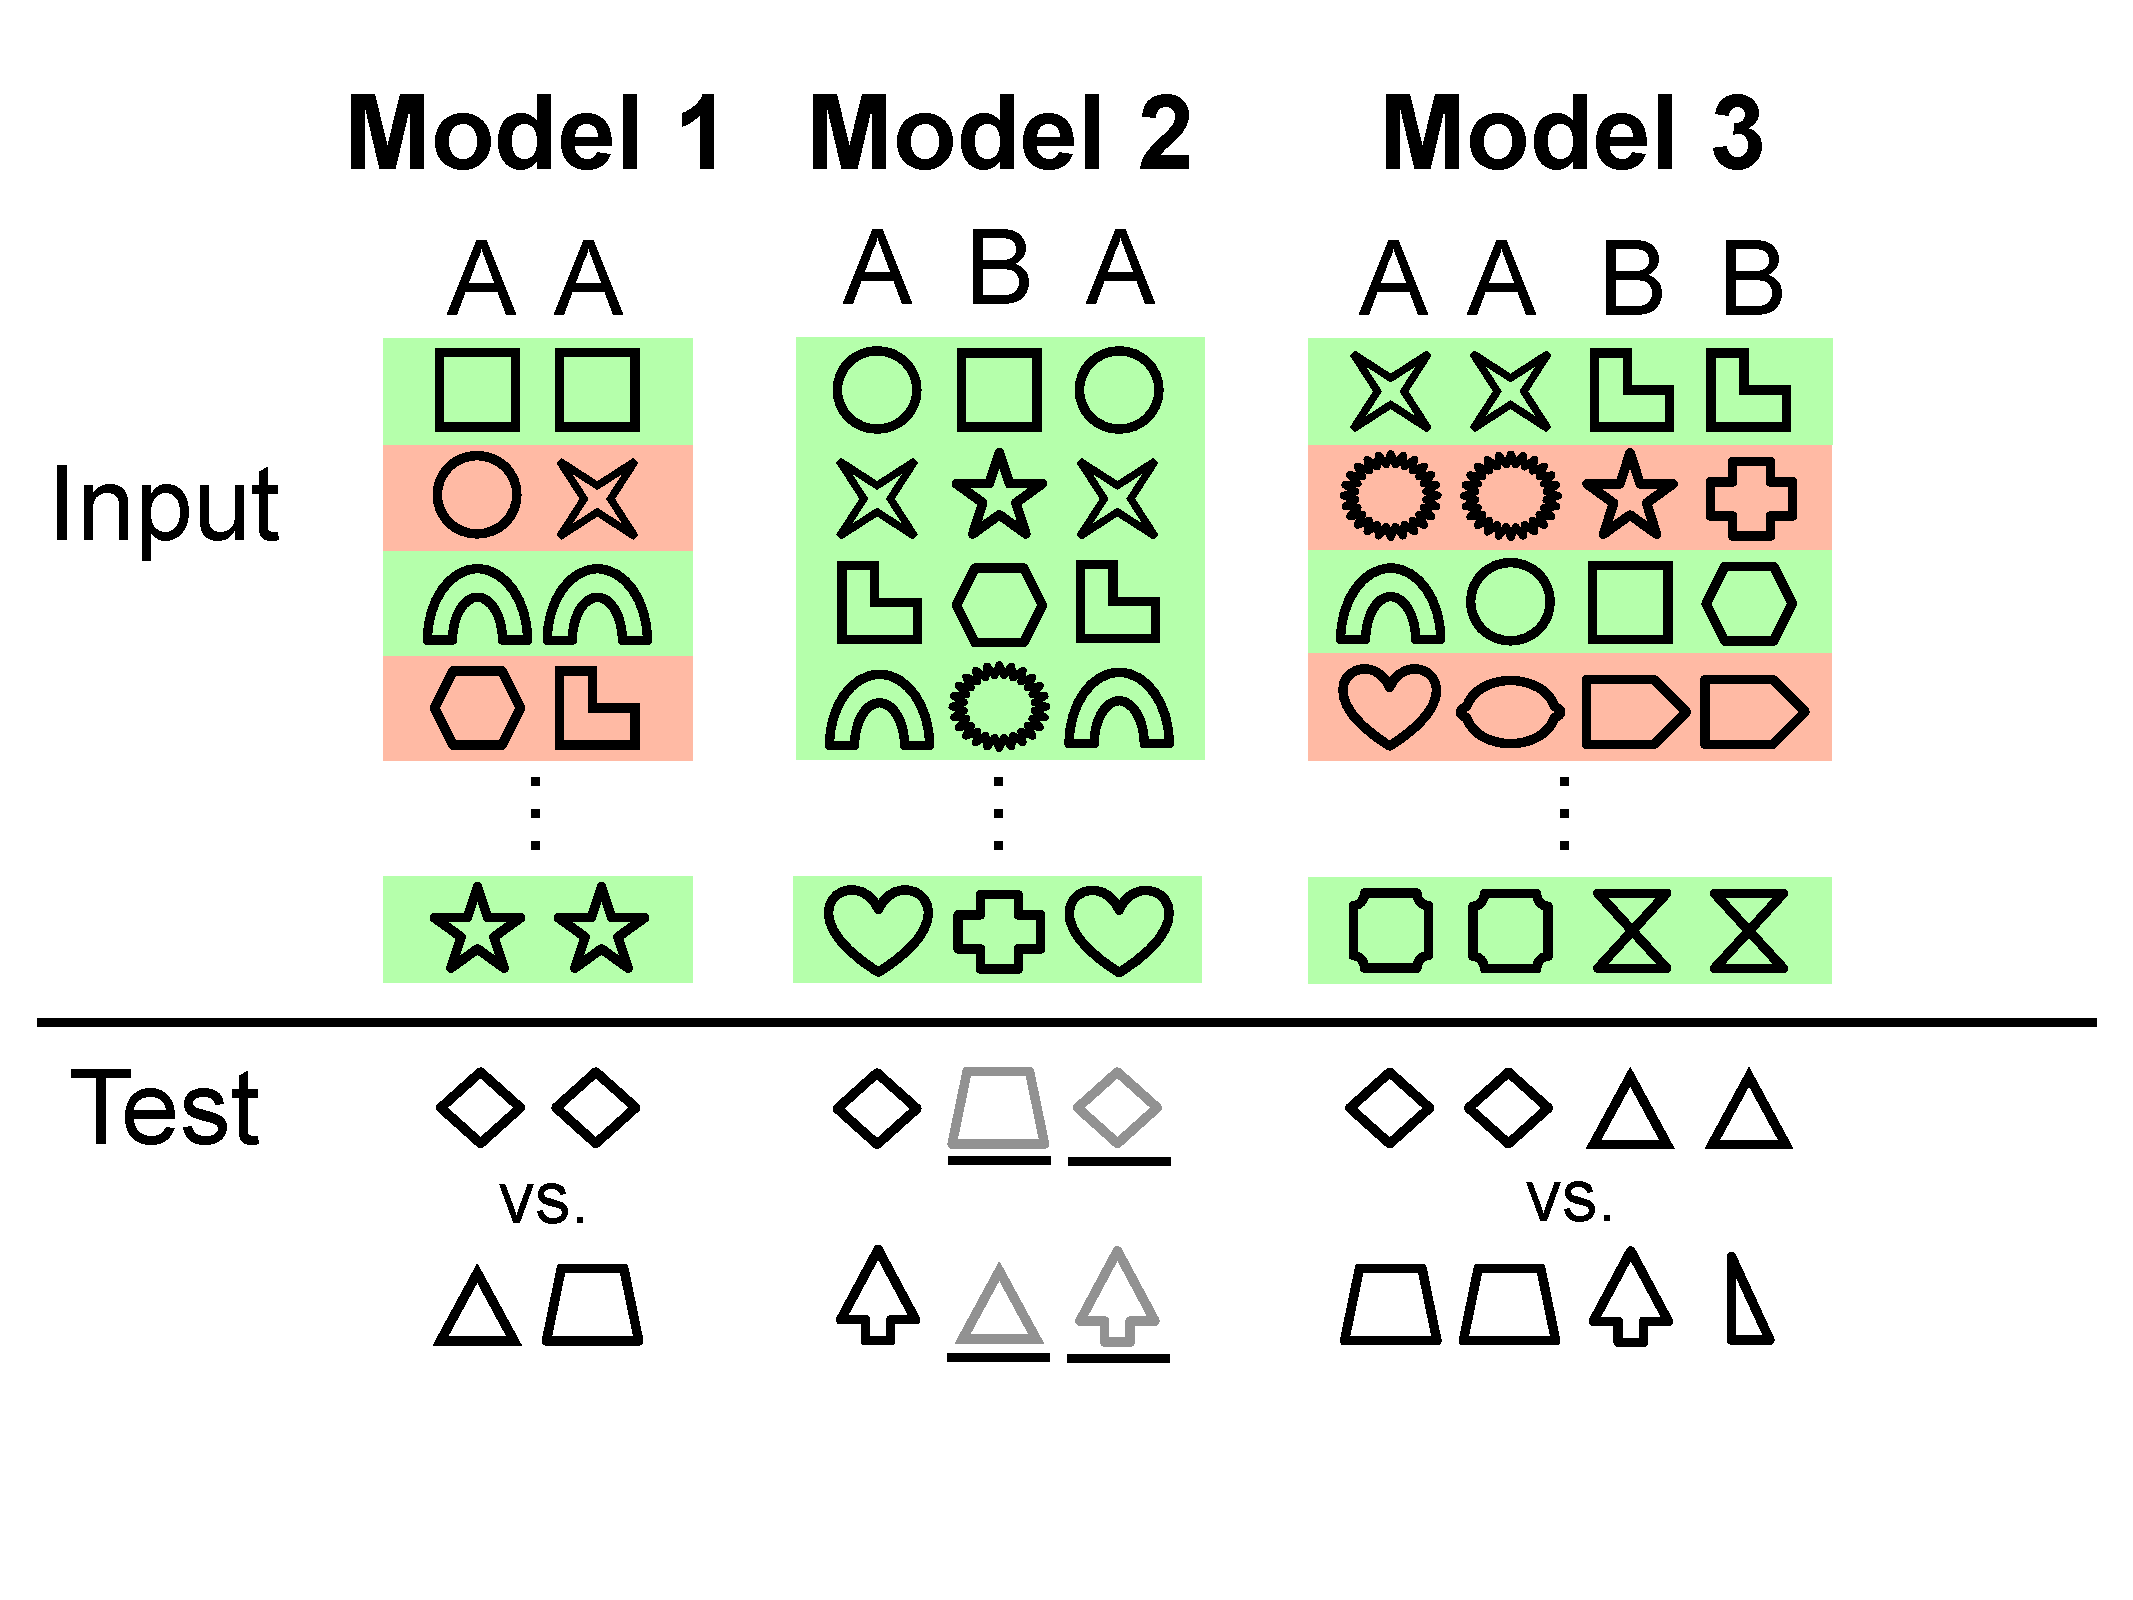
\includegraphics[scale=0.20]{modelfigv1.pdf}
\caption{Relational reasoning tasks. Green and red mark positive and negative training examples, respectively. The sequential task (Model~2) uses only positive instances, and a model succeeds if, prompted with $\alpha$, it produces a sequence $\beta \ \alpha$ for $\beta \neq \alpha$. For the hierarchical task (Model~3), we show that a model trained on the basic task (Model~1) is effective with no additional training.}
\label{fig:tasks}
\end{figure}

We revisit this debate here, adopting stringent criteria for generalization and considering a broader range of representations across three models. We model three cases of identity-based reasoning that have featured prominently in discussions of the role of symbols in relational reasoning (\figref{fig:tasks}): (1) learning to discriminate pairs of objects that exemplify the relation \emph{same} or \emph{different}, (2) learning sequences with repeated \emph{same} elements \cite{marcus:1999}, and (3) learning to distinguish hierarchical \emph{same} and \emph{different} relations in a context with pairs of pairs exemplifying these relations \cite{Premack:1983}. This last problem is more challenging and requires vastly more data. We show how using pretraining -- an active area of development in recent artificial intelligence research \cite{CollobertWeston:2011,Mikolov-etal:2013,pennington-socher-manning:2014:EMNLP2014,Peters-etal:2018,Devlin-etal:2019} -- can help achieve far faster learning.

Across these three models, we find strong support for their ability to learn equality relations. These results should serve to revise the conclusions of the earlier debate. Marcus and colleagues \cite{marcus:1999,marcus:2001} showed experimentally that neural networks using feature representations cannot generalize to binary features unseen in training. We agree with this claim (and support it with a direct mathematical argument in \appref{app:generalization}). However, they concluded from this result that neural networks will need to have primitive symbolic operators to solve hard relational reasoning tasks. On this point, we disagree. Our experiments show that networks without these primitives can solve a range of these tasks, as long as they use non-featural representations. Overall, these findings suggest that essential aspects of symbolic reasoning can emerge from entirely data-driven, non-symbolic learning processes.

\section{Designing theoretical models of equality learning}

We begin by discussing two critical design considerations for our models: (1) the standards for generalization by which models should be evaluated and (2) the type of representations they should use. To summarize this discussion: we select generalization tasks with fully disjoint training and test vocabularies to provide the most stringent test of generalization. Further, we adopt both randomly initialized non-featural representations and pretrained non-featural representations for our subsequent models, and we show analytically that other kinds of representations are more limited in their capacity to make successful out-of-sample generalizations.


\subsection{Generalization}

The standard approach to training and evaluating neural networks is to choose a dataset, divide it randomly into training and assessment sets, train the system on the training set, and then use its performance on the assessment set as a proxy for its capacity to generalize to new data.

The standard approach is fine for many purposes, but it raises concerns in a context in which we are trying to determine whether a network has truly acquired a global solution to a target function. In particular, where there is any kind of overlap between the training and assessment vocabularies (primitive elements), we can't rule out that the network might be primarily taking advantage of idiosyncrasies in the underlying dataset to effectively cheat -- to memorize aspects of the training set and learn a local approximation of the target function that happens to provide traction during assessment.

To address this issue, \update{we follow \citet{marcus:1999} in proposing} that networks must be evaluated on assessment sets that are completely disjoint in every respect from the train set, all the way down to the entities involved. For example, below, we train on pairs $(a, a)$ and $(a, b)$, where $a$ and $b$ are representations from a train vocabulary $V_{T}$. At test time, we create a new assessment vocabulary $V_{A}$, derive equality and inequality pairs $(\alpha, \alpha)$ and $(\alpha, \beta)$ from that vocabulary, and assess the trained network on these new examples. In adopting these methods, we get a clear picture of the system's capacity to generalize, and we can safely say that its performance during assessment is a window into whether a global solution to identity has been learned. This is a very challenging setting for any machine learning model. For the sequential same--different task, we will see that it even requires us to departure from usual model formulations.

\subsection{Representations}\label{sec:representations}

\newcommand{\mysquare}{

\begin{tikzpicture}[scale=0.5]
 \node[rectangle, fill=red!100, minimum height=3mm, minimum width=3mm]{};
\end{tikzpicture}}

\newcommand{\bluetriangle}{


\begin{tikzpicture}[scale=0.25]
 \node[regular polygon,regular polygon sides=3, fill=blue!100, inner sep=2pt]{};
\end{tikzpicture}}
\newcommand{\redtriangle}{

\begin{tikzpicture}[scale=0.5]
 \node[regular polygon,regular polygon sides=3, fill=red!100, inner sep=2pt]{};
\end{tikzpicture}}
\newcommand{\bluesquare}{

\begin{tikzpicture}[scale=0.5]
 \node[regular polygon,regular polygon sides=4, fill=blue!100, minimum height=3mm, minimum width=3mm]{};
\end{tikzpicture}}
\newcommand{\redsquare}{

\begin{tikzpicture}[scale=0.5]
 \node[regular polygon,regular polygon sides=4, fill=red!100, minimum height=3mm, minimum width=3mm]{};
\end{tikzpicture}}
\newcommand{\bluepentagon}{

\begin{tikzpicture}[scale=0.5]
 \node[regular polygon,regular polygon sides=5, fill=blue!100, minimum height=3mm, minimum width=3mm]{};
\end{tikzpicture}}
\newcommand{\redpentagon}{

\begin{tikzpicture}[scale=0.5]
 \node[regular polygon,regular polygon sides=5, fill=red!100, minimum height=3mm, minimum width=3mm]{};
\end{tikzpicture}}

\newcommand{\myrectangle}{

\begin{tikzpicture}[scale=0.25]
 \node[rectangle, fill=blue!100, minimum height=3mm, minimum width=5mm]{};
\end{tikzpicture}}

\newcommand{\mypentagon}{

\begin{tikzpicture}[scale=0.5]
 \node[regular polygon,regular polygon sides=5, minimum height=4mm, fill=red!100]{};
\end{tikzpicture}}


\newcommand{\mypolygon}{

\begin{tikzpicture}[scale=0.5]
 \node[regular polygon,regular polygon sides=7, minimum height=4mm, fill=blue!100]{};
\end{tikzpicture}}


\begin{figure*}[t!]
\setlength{\arraycolsep}{2pt}
\centering
\small
\begin{subfigure}[t]{0.1\textwidth}
 \centering
 \begin{tabular}[b]{@{} c @{}}
  \midrule
  \bluetriangle \\
  \redtriangle \\
  \bluesquare \\
  \redsquare \\
  % \bluepentagon \\
   $\vdots$ \\
  \redpentagon \\
  \bottomrule
 \end{tabular}
 \caption{}
 \label{fig:entities}
\end{subfigure}
\hfill
\begin{subfigure}[t]{0.25\textwidth}
 \centering
 \renewcommand{\arraystretch}{1.18}
 $\begin{array}[b]{*{6}{c}}
   \toprule
   \bluetriangle & \redtriangle & \bluesquare & \redsquare & \bluepentagon & \redpentagon \\
   \midrule
   1 & 0 & 0 & 0& 0& 0 \\
   0 & 1 & 0 & 0& 0& 0 \\
   0 & 0 & 1 & 0& 0& 0 \\
   0 & 0 & 0 & 1& 0& 0 \\
   % 0 & 0 & 0 & 0& 1&0 \\
   \multicolumn{6}{c}{\vdots} \\
   0 & 0 & 0 & 0& 0& 1 \\
  \bottomrule
 \end{array}$
 \caption{Localist.}
 \label{fig:reps:localist}
\end{subfigure}
\hfill
\begin{subfigure}[t]{0.14\textwidth}
 \centering
 \renewcommand{\arraystretch}{1.18}
 $\begin{array}[b]{*{3}{r}}
   \toprule
   \rotatebox{90}{red} & \rotatebox{90}{blue} & \rotatebox{90}{sides}\\
   \midrule
   0 & 1 & 3  \\
   1 & 0 & 3  \\
   0 & 1 & 4  \\
   1 & 0 & 4 \\
   % 0 & 1 & 5 \\
   \multicolumn{3}{c}{\vdots} \\
   1 & 0 & 5 \\
   \bottomrule
 \end{array}$
 \caption{Distributed.}
 \label{fig:reps:symbolic}
\end{subfigure}
\hfill
\begin{subfigure}[t]{0.2\textwidth}
 \centering
 \renewcommand{\arraystretch}{1.18}
 $\begin{array}[b]{rr}
   \toprule
   d_{1} & d_{2} \\
   \midrule
   -0.4 &  0.2 \\
   0.2 &  -0.2 \\
   0.4 &  0.0 \\
   -0.2 &  -0.0 \\
   % 0.2 &  0.4 \\
   \multicolumn{2}{c}{\vdots} \\
   0.5 &  0.2 \\
   \bottomrule
 \end{array}$
 \caption{Random.}
 \label{fig:reps:random}
\end{subfigure}
\hfill
\begin{subfigure}[t]{0.2\textwidth}
 \centering
 \renewcommand{\arraystretch}{1.18}
 $\begin{array}[b]{rr}
   \toprule
   d_{1} & d_{2} \\
   \midrule
   -1.3 &  0.4 \\
   -0.1 &  -1.1 \\
   -0.9 &  1.2 \\
   0.6 &  -0.6 \\
   %-0.9 &  2.1 \\
   \multicolumn{2}{c}{\vdots} \\
   1.2 &  -0.1 \\
   \bottomrule
 \end{array}$
 \caption{Pretrained.}
 \label{fig:reps:pretrained}
\end{subfigure}

\vspace{12pt}

\begin{subfigure}[t]{0.48\linewidth}
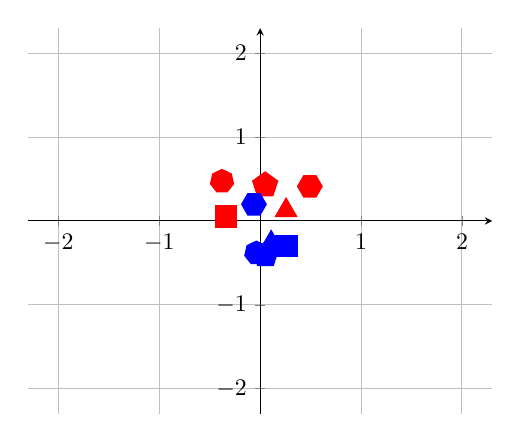
\begin{tikzpicture}[scale=0.86]
\begin{axis}[
 title={},
 grid=major,
axis lines=middle,
 no markers,
 every axis plot/.append style={ultra thick},
 xmin=-2.3, xmax=2.3,
 ymin=-2.3, ymax=2.3,
 xtick={-2,-1,0,1,2},
 ytick={-2,-1,0,1,2}
]
\node[regular polygon,regular polygon sides=3, fill=red!100,inner sep=2pt] at (axis cs:0.25644314, 0.12540874) {};
\node[regular polygon,regular polygon sides=4, fill=blue!100] at (axis cs:0.25999054, -0.29644176) {};
\node[regular polygon,regular polygon sides=5, fill=red!100] at (axis cs:0.049219638, 0.42767277) {};
\node[regular polygon,regular polygon sides=6, fill=blue!100] at (axis cs:-0.061883904, 0.19825003) {};
\node[regular polygon,regular polygon sides=7, fill=red!100] at (axis cs:-0.37857392, 0.47314683) {};
\node[regular polygon,regular polygon sides=3, fill=blue!100,inner sep=2pt] at (axis cs:0.10887167, -0.26070255) {};
\node[regular polygon,regular polygon sides=4, fill=red!100] at (axis cs:-0.34162185, 0.050839007) {};
\node[regular polygon,regular polygon sides=5, fill=blue!100] at (axis cs:0.05225141, -0.4067908) {};
\node[regular polygon,regular polygon sides=6, fill=red!100] at (axis cs:0.49225715, 0.4129299) {};
\node[regular polygon,regular polygon sides=7, fill=blue!100] at (axis cs:-0.038552105, -0.38253385) {};
 %\node[regular polygon,regular polygon sides=3, fill=blue!100,inner sep=2pt] at (axis cs:-0.35932082, 0.17664503) {};
 %\node[regular polygon,regular polygon sides=3, fill=red!100,inner sep=2pt] at (axis cs: 0.23422007, -0.23213634) {};
 %\node[regular polygon,regular polygon sides=4, fill=blue!100] at (axis cs:0.4148342 , 0.02179685) {};
 %\node[regular polygon,regular polygon sides=4, fill=red!100] at (axis cs:-0.19870198, -0.02996263) {};
 %\node[regular polygon,regular polygon sides=5, fill=blue!100] at (axis cs: 0.23975432 , 0.40730593) {};
 %\node[regular polygon,regular polygon sides=5, fill=red!100] at (axis cs:0.49842966 , 0.17170991) {};
\end{axis}
\end{tikzpicture}
 \caption{The matrix in \figref{fig:reps:random} (before pretraining).}

 \label{fig:tsne-random}
\end{subfigure}
\hfill
\begin{subfigure}[t]{0.48\linewidth}
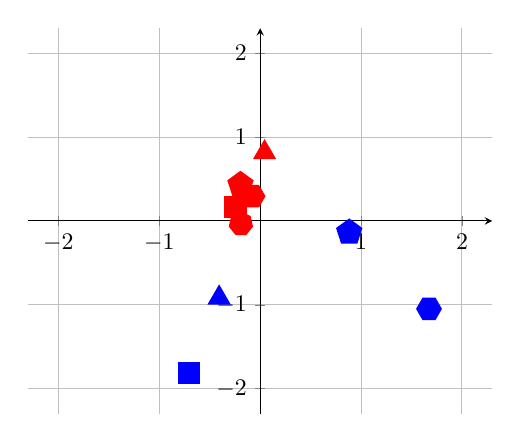
\begin{tikzpicture}[scale=0.86]
\begin{axis}[
 title={},
 no markers,
 grid=major,
axis lines=middle,
 every axis plot/.append style={ultra thick},
 xmin=-2.3, xmax=2.3,
 ymin=-2.3, ymax=2.3,
 xtick={-2,-1,0,1,2},
 ytick={-2,-1,0,1,2}
]
\node[regular polygon,regular polygon sides=3, fill=red!100,inner sep=2pt] at (axis cs:0.043389633, 0.8164206) {};
\node[regular polygon,regular polygon sides=4, fill=blue!100] at (axis cs:-0.7053148, -1.812479) {};
\node[regular polygon,regular polygon sides=5, fill=red!100] at (axis cs:-0.19551103, 0.4328718) {};
\node[regular polygon,regular polygon sides=6, fill=blue!100] at (axis cs:1.6731963, -1.0493283) {};
\node[regular polygon,regular polygon sides=7, fill=red!100] at (axis cs:-0.19127868, -0.034780912) {};
\node[regular polygon,regular polygon sides=3, fill=blue!100,inner sep=2pt] at (axis cs:-0.40698338, -0.91700864) {};
\node[regular polygon,regular polygon sides=4, fill=red!100] at (axis cs:-0.24272422, 0.16861145) {};
\node[regular polygon,regular polygon sides=5, fill=blue!100] at (axis cs:0.88247913, -0.13587654) {};
\node[regular polygon,regular polygon sides=6, fill=red!100] at (axis cs:-0.075923756, 0.29488102) {};
\node[regular polygon,regular polygon sides=7, fill=blue!100] at (axis cs:2.1035564, -2.6820786) {};
 %\node[regular polygon,regular polygon sides=3, fill=blue!100,inner sep=2pt] at (axis cs:-1.2906312,  0.36732233]) {};
 %\node[regular polygon,regular polygon sides=3, fill=red!100,inner sep=2pt] at (axis cs: -0.09487347, -1.1454606) {};
 %\node[regular polygon,regular polygon sides=4, fill=blue!100] at (axis cs:-0.8569037 , 1.1844875) {};
 %\node[regular polygon,regular polygon sides=4, fill=red!100] at (axis cs: 0.56387985, -0.61090606) {};
 %\node[regular polygon,regular polygon sides=5, fill=blue!100] at (axis cs:-0.94791865, 2.0959575) {};
 %\node[regular polygon,regular polygon sides=5, fill=red!100] at (axis cs:1.2290089, -0.08361815) {};
\end{axis}
\end{tikzpicture}
 \caption{The matrix in \figref{fig:reps:pretrained} (after pretraining).}
 \label{fig:tsne-pretrained}
\end{subfigure}

\caption{Each matrix is a method for representing the shapes in \figref{fig:entities}, where each row is a vector representation of one shape. Localist and distributed are feature representations where each vector dimension encodes the value of a single property. Random and pretrained are non-featural representations where the values of properties are encoded implicitly in two dimensions. Random representations and localist representations encode only identity, whereas distributed representations and pretrained representations encode color and number of sides.}
\label{fig:reps}
\end{figure*}

% \updatea{
Essentially all modern machine learning models represent objects using vectors of real numbers. However, there are important differences in how these vectors are used to encode the properties of objects. In this section, we characterize two broad approaches to such property encoding -- \tech{featural representations} and \tech{non-featural representations} -- and argue that the differences between them have not been given sufficient attention in the debate about the ability of neural networks to perform relational reasoning.

To ground our discussion, we consider a hypothetical universe of blocks which vary by shape and color. \Figref{fig:entities} is a partial view of them, and \figref{fig:reps:localist}--\figref{fig:reps:pretrained} present four different ways of encoding the properties of these objects in vectors.

\subsubsection{Featural Representations}

The defining characteristic of \tech{featural} vector representations is that each dimension encodes the value of a single property. The properties can be binary, integer-valued, or real-valued.

We use the term \tech{localist} for the special case of featural representations in which only identity properties are represented and there is an identity property corresponding to each object. In \figref{fig:reps:localist}, each column represents the property of being an object, and every object is represented as a vector that has a single unit with value 1. There is no shared structure across objects; all are equally (un)related to each other as far as the model is concerned.

A featural representation that is not localist is often called a \tech{distributed representation}. Here, column dimensions encode specific properties of objects. Coming back to our universe of blocks, we can represent the properties of being red and being blue with two different binary features, and the property of having a certain number of sides as a single analog feature, as in \figref{fig:reps:symbolic}. Unlike with localist representations, objects in this space can have complex relationships to each other, as encoded in the shared structure given by the columns.

Featural representations -- both localist and distributed -- have the appealing property that they are easy for researchers to interpret because of the tight correspondence between column dimensions and properties. However, this transparency actually inhibits neural networks from discovering general solutions; such models work far better with representations that have property values implicitly encoded in the abstract structure of the vector space. We demonstrate this result analytically in \appref{app:generalization} for the case of binary features. The core insight is that networks cannot learn anything about column dimensions that are not represented in their training data; whatever weights are associated with those dimensions are unchanged by the learning process, so predictions about those dimensions remain random at test time. The density of non-featural representations helps to avoid this limitation, and pretraining can fully overcome it.

\subsubsection{Non-Featural Representations}

A \tech{non-featural representation} is a vector that encodes property values implicitly across many dimensions. Perhaps the simplest non-featural representations are \tech{completely random} vectors, as in \figref{fig:reps:random}. Random representations can be seen as the non-featural counterpart to localist representations. In both of these representation schemes, all the objects are equally (un)related to each other, since column-wise patterns are unlikely in random representations and, to the extent that they are present, they exist completely by chance. However, in random representations, all the column dimensions can contribute meaningfully to identifying objects, whereas a localist representation has only one vector unit that determines the identity of any given object object.

Random representations are a starting point that encodes object identity. To encode more diverse information, we can \tech{pretrain} random representations via a learning process. This will imbue them with rich structure that implicitly encodes property values across many dimensions. \Figref{fig:reps:pretrained} provides a simple example. This matrix is the results of pretraining the representations in \figref{fig:reps:random} on the task of predicting whether the object is blue, whether the object is red, and the number of sides the object has. (\Appref{app:pretraining} provides technical details on our pretraining approach.) Superficially, the two matrices look equally random. However, this is only because our pretraining process leads to property values being implicitly represented by linear structures in the vector representation space. The random representations in \figref{fig:tsne-random} have no such linear structure (e.g., no line separates blue and red objects). However, the pretrained representations in \figref{fig:tsne-pretrained} have a structure such that straight lines can be drawn to separate objects by color and by number of sides.

Pretraining need not be restricted to input representations. All the parameters of a model can be pretrained. In this setting, a small amount of task-specific training (often called ``fine-tuning'') might suffice. This offers the possibility that networks might be used as modular components to solve more complex tasks. We realize this possibility in \secref{sec:premack}, where a model pretrained on a simple equality is used as a modular component to compute hierarchical equality.


% \subsubsection{The Superiority of Non-Featural Representations}

% We argue that non-featural representations are superior to featural ones for two reasons: (1) non-featural representations are more biologically plausible than feature representations; and (3) featural representations can seriously inhibit the ability of neural networks to generalize to unseen examples.

% From a biological perspective, we might want the representations we feed our artificial neural networks to be similar to perceptual neural representations in biological neural networks. We believe it is obvious that biological neural representations are such that property values are not explicitly encoded or localized to the activity of a single neuron. For example, when a human looks at a red square block that is red, the property of being red is not encoded in the activity of a single neuron in the vision system, but instead is encoded in the activations of many neurons. This is a property that is shared with pretrained non-featural representations, but not with feature representations, where property values are explicit and localized.



% \subsubsection{On the Symbolic/Non-Symbolic Distinction}


% \subsection{The current paper}

\section{Model 1: Same--different relations}\label{sec:equality}

In our first model, we consider whether a supervised, feed-forward classification model can learn equality (and inequality) relations in the strict setting we describe above: random representations with disjoint generalization examples.

\subsection{Model}

Our basic model for equality is a feed-forward neural network with a single hidden representation layer:
%
\begin{align}
h &= \ReLU([a;b]W_{xh} + b_{h}) \label{eq:x2h}\\
y &= \softmax(hW_{hy} + b_{y}) \label{eq:h2y}
\end{align}
%
The input is a pair of vectors $(a, b)$, each of dimension $m$, which correspond to the two stimulus objects. These vectors are non-featural representations that do not have features encoding properties of the objects or their identity. These are concatenated to form a single vector $[a;b]$ of dimension $2m$, which is the simplest way of merging the two representations to form a single input.

This representation is multiplied by a matrix of weights $W_{xh}$ of dimension $2m \times n$ and a bias vector $b_{h}$ of dimension $n$ is added to this result, where $n$ is the hidden layer dimensionality. These two steps create a linear projection of the input representation, and the bias term is the value of this linear projection when the input representation is the zero vector. Then, the non-linear activation function $\ReLU$ ($\ReLU(x) = \max(0, x)$) is applied element-wise to this linear projection. This non-linearity is what gives the neural model more expressive power than a logistic regression \citep{Cybenko:1989,Hornik:Stinchcombe:White:1989}. The result is the hidden representation $h$.

The hidden representation is the input to the classification layer: $h$ is multiplied by a second matrix of weights $W_{hy}$, dimension $n \times 2$, and a bias term $b_{y}$ (dimension 2) is added to this. This second bias term encodes the probabilities of each class when the hidden representation is 0. The result is fed through the softmax activation function: $\softmax(x)_{i} = \frac{\exp{x_{i}}}{\sum_{j} \exp{x_{j}}}$. This creates a probability distribution over the classes (positive and negative). For a given input, the model computes this probability distribution and the input is categorized as the class with the higher probability.

During training, this model is presented with positive and negative labeled examples and the parameters $W_{xh}$, $W_{hy}$, $b_{y}$, and $b_{h}$ are learned using back propagation with a cross entropy loss function. \update{This function is defined as follows, for a corpus of $N$ examples and $K$ classes:
%
\begin{equation}
\max(\theta)
\quad
\frac{1}{N}
\sum_{i=1}^{N}
\sum_{k=1}^{K}
y^{i,k} \log(h_{\theta}(i)^{k})
\end{equation}
%
where $\theta$ abbreviates the model parameters ($W_{xh}$, $W_{hy}$, $b_{y}$, $b_{h}$), $y^{i,k}$ is the actual label for example $i$ and class $k$, and $h_{\theta}(i)^{k}$ is the corresponding prediction.}

During testing, this model is tasked with categorizing inputs unseen during training. It is straightforward to show that a network like this is capable of learning equality as we have defined it. \Appref{app:equality-solution} provides an analytic solution to the equality relation using this neural model. \update{Here we illustrate with a small example network that maps all identity pairs to $[0.5, 0.5]$ and all non-identity pairs to $[y, 1-y]$ where $y > 0.5$, which supports a trivial classification rule:
%
\setlength{\arraycolsep}{4pt}
\begin{equation}
\softmax\left(
  \ReLU\left(
    [a;b]
    \left(
      \begin{array}[c]{@{} *{4}{r} @{}}
        1 & 0 & -1 & 0 \\
        0 & 1 & 0 & -1 \\
        -1 & 0 & 1 & 0 \\
        0 & -1 & 0 & 1
      \end{array}
    \right)
    +
    \mathbf{0}
  \right)
  \left(
    \begin{array}[c]{@{} r r @{}}
      1 & 0 \\
      1 & 0\\
      1 & 0\\
      1 & 0\\
    \end{array}
  \right)
  +
  \mathbf{0}
\right)
\end{equation}}

\begin{figure*}[tp]
\centering
\begin{subfigure}[t]{0.48\linewidth}
 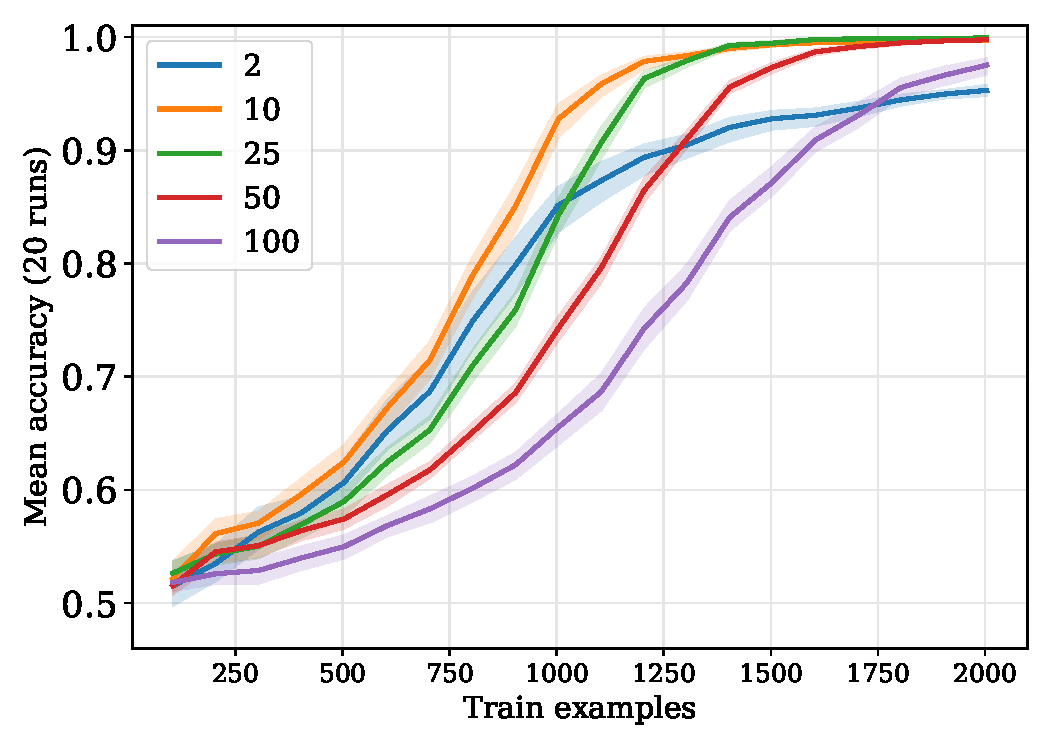
\includegraphics[width=1\linewidth]{../fig/equality-train_size-embed_dim-hidden_dim=100.pdf}
 \vspace{-4mm}
 \caption{Results for a model in which the hidden layer has dimensionality $100$. The lines correspond to different dimensions for the entities $a$ and $b$ in the input pairs $(a, b)$. These models largely pass 90\% accuracy with 1,000 training examples and reach (near) perfection by 1,250.}
 \label{fig:equality--smallresults}
\end{subfigure}
\hfill
\begin{subfigure}[t]{0.48\linewidth}
 \centering
 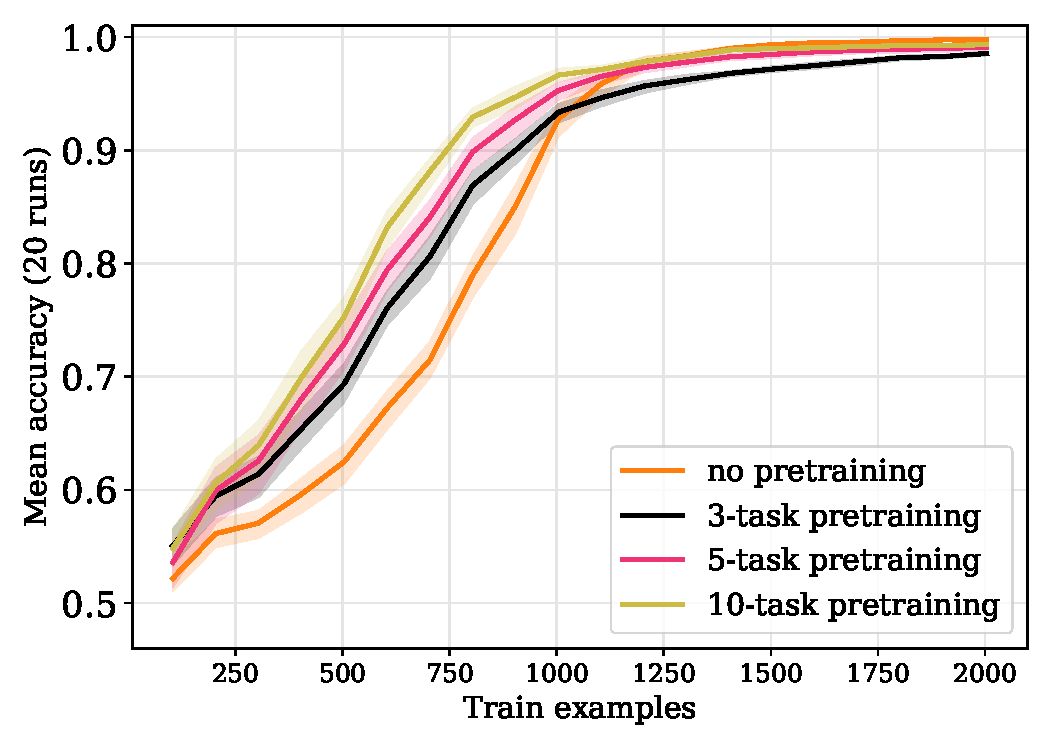
\includegraphics[width=1\linewidth]{../fig/equality-pretrain-compare-train_size-pretrained-embed_dim=None.pdf}
 \caption{\update{Results where random representations are grounded in a number of property domains via pretraining learning tasks. The `no pretraining' model is the best of the models at left (10-dimensional embeddings, 100-dimensional hidden layers), repeated to facilitate comparisons. The pretraining models use those same dimensionalities.}}
 \label{fig:basic-equality-pretrain}
\end{subfigure}
\caption{Same--different results with and without pretraining.}
\end{figure*}


This result shows that equality in our sense is learnable in principle, but it doesn't resolve the question of whether networks can find this kind of solution given finite training data. To address this, we train the network on a stream of pairs of random vectors. Half of these are identity pairs $(a, a)$, labeled with $1$, and half are non-identity pairs $(a, b)$, labeled with $0$. Trained networks are assessed on the same kind of balanced dataset, with vectors that were never seen in training so that, as discussed earlier, we get a clear picture of whether they have found a generalizable solution. Further optimization details are in \appref{app:optimization}.



\subsection{Results}

\Figref{fig:equality--smallresults} presents typical results. This is for the case where the hidden layer dimensionality is $100$, and we plot results for different embedding dimensionalities $m$ and different amounts of training data. The picture is comparable with hidden dimensionalities at 10, 25, and 50, but those models require more training data to reach (near) perfect performance (\appref{app:model1-results}).

While all the networks in \figref{fig:equality--smallresults} reach above-chance performance almost immediately, they require upwards of 1,000 examples to truly solve these tasks. We additionally ran the above experiments using random representations that were pretrained using a linear classifier for 0, 3, 5, or 10 different feature discrimination tasks. For example, following \figref{fig:reps}, a two-task model would be trained to encode the properties of color, number of sides, and size.

\Figref{fig:basic-equality-pretrain} summarizes the results of these experiments for 10-dimensional embeddings and 100-dimensional hidden representations, as this seems to be the network that learns the fastest with random inputs. Interestingly, we see a clear speed-up, with more pretraining tasks resulting in the largest gains; by grounding our representations in ``property domains'' (as represented by the different task dimensions), we imbue them with implicit structure that makes learning easier.

\subsection{Discussion}

Our assessment pairs have nothing in common with the training pairs except insofar as both involve vectors of real numbers of the same dimensionality. During training, the network is told (via labels) which pairs are equality pairs and which are not, but the pairs themselves contain no information about equality per se. It thus seems fair to us to say that these networks have learned equality, or at least how to simulate that relation with near perfect accuracy. Further, the use of representations that are structured by pretraining results in faster learning.

\section{Model 2: Sequential same--different (ABA task)}\label{sec:lms}

Our first model is simple and successfully learns equality. However, this model is supervised with both positive and negative evidence. In the initial debate around these issues, supervision with negative evidence was dismissed as an unreasonably strong learning regime \citep[e.g.,][]{marcus:1999a}. While this argument likely holds true for language learning \citep[in which supervision is generally agreed not to be binary or direct;][]{brown:1970,chouinard2003}, it is not necessarily true for learning more generally. Nevertheless, learning of sequential rules without negative feedback is possible for infants \cite{marcus:1999,rabagliati:2019}. In experiments of this type, infants are presented with a set of positive examples. Our next model explores whether neural network models can learn this task in a challenging regime with no negative supervision.

\subsection{Model}

To explore learning with only positive instances, we use neural language models. These models are sequential: at each timestep, they predict an output given their predictions about the preceding timesteps. As typically formulated, the prediction function is just a classifier: at each timestep, it predicts a probability distribution over the entire vocabulary of options, and the item with the highest probability is chosen as a symbolic output. This output becomes the input at the next timestep, and the process continues.

This formulation will not work in situations in which we want to make predictions about test items with an entirely disjoint vocabulary from the training sample. The classifier function will get no feedback about these out-of-vocabulary items during training, and so it will never predict them during testing. To address this issue, we reformulate the prediction function. Our proposal is to have the model predict output vector representations -- instead of discrete vocabulary items -- at each timestep. During training, the model is trained to minimize the distance between these output predictions and the representations of the actual output entities. During assessment, we take the prediction to be the item in the entire vocabulary (training and assessment) whose representation is closest to the predicted vector (in terms of Euclidean distance). This fuzzy approach to prediction creates enough space for the model to predict sequences from an entirely new vocabulary.

The specific model we use for this is as follows:
%
\begin{align}
h_{t} &= \LSTM(x_{t}, h_{t-1}) \label{eq:lstm-recur}\\
y_{t} &= h_{t}W + b\label{eq:lstm-predict}
\end{align}
%
This holds for $t > 0$, and we set $h_{0} = \mathbf{0}$. $\LSTM$ is a long short-term memory cell \cite{hochreiter:1997}. Full details on these cells are given in \appref{sec:analyticlm}.

The input is a sequence of vectors $x_1, x_2, x_3, \dots$, each of dimension $m$, which correspond to a sequence of stimulus objects. These vectors are, again, non-featural representations that do not have features encoding properties of the objects or their identity.


At each timestep $t$, the input vector $x_t$ is fed into the $\LSTM$ cell along with the previous hidden representation $h_{t-1}$. The defining feature of an $\LSTM$ is the ability to decide whether to store information from the current input, $x_t$, and whether to remember or forget the information from the previous timestep $h_{t-t}$. The output of the $\LSTM$ cell is the hidden representation for the current time step $h_t$. The dimension of the hidden representations is $n$. The hidden representation is multiplied by a matrix $W$ with dimensionality $n \times m$ to produce $y_t$. This result, $y_t$, is a linear projection of the hidden representation into the input vector space, which is necessary because $y_t$ is a prediction of what the next input, $x_{t+1}$, will be.

% \update{
The objective function is as follows:
%
\begin{equation}
\max(\theta)
\quad
-\frac{1}{N}
\sum_{i=1}^{N}
\sum_{t=1}^{T_{i}}
\left\| h_{\theta}\left(x^{i, 0:{t-1}}\right) - x^{i,t} \right\|^{2}
\end{equation}
%
for $N$ examples. Here, $T_{i}$ is the length of example $i$. As before, $\theta$ abbreviates the parameters of the model as specified in \dasheg{eq:lstm-recur}{eq:lstm-predict}. We use $h_{\theta}(x^{i, 0:{t-1}})$ for the vector predicted by the model for example~$i$ at timestep~$t$, which is compared to the actual vector at timestep $t$ via squared Euclidean distance (i.e., the mean squared error).
% As noted above, this is an unusual formulation for a language model. The usual version essentially treats every timestep as involving a classification decision, with a cross-entropy loss. We cannot adopt this because of our goal of using unseen vocabulary items at test time. % MCF: seemed redundant

\Appref{sec:analyticlm} provides an analytic solution to the ABA task using this model. To see how well the model performs in practice, we trained networks on sequences \texttt{<s> a b a </s>}, where $\texttt{b} \neq \texttt{a}$. We show the network every such sequence during training, from an underlying vocabulary of 20 items (creating a total of 380 examples). To assess how well the model learns this pattern, we seed it with \texttt{<s> x} where \texttt{x} is an item from a disjoint vocabulary from that seen in training, and we say that a prediction is accurate if the model continues with \texttt{y x </s>}, where \texttt{y} is any character (from the training or assessment vocabulary) except \texttt{x}.

\subsection{Results}

\Figref{fig:fuzzy-lm-results} shows the results for a model with a 100-dimensional hidden representation. As before, the results are comparable for smaller networks. Unlike for the previous equality experiments, we found that we had to allow the model to experience multiple epochs of training on the same set in order to succeed. \figref{fig:fuzzy-lm-pretrain-results} shows results with pretrained representations across a range of different tasks (as in Model~1); these yielded no increase in performance.
% , and hence the x-axis counts examples in terms of epochs of learning on our fixed set of 380 examples.  % MCF; not correct anymore right?

\begin{figure*}[tp]
\centering
\begin{subfigure}[t]{0.48\textwidth}
 \centering
 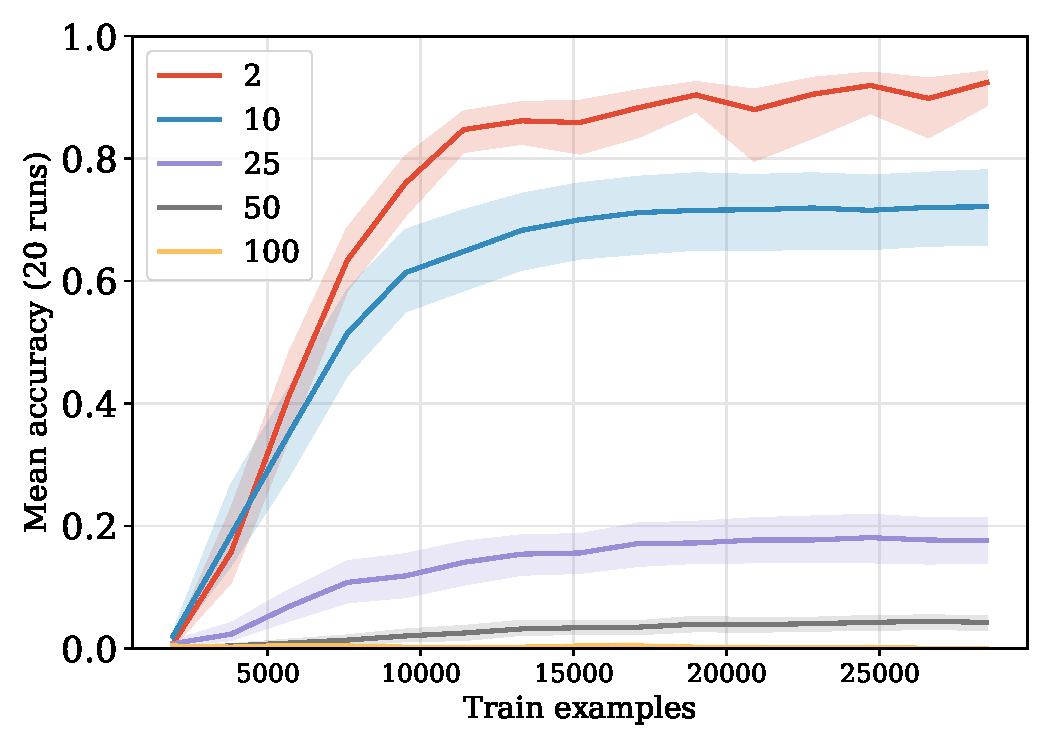
\includegraphics[width=1\linewidth]{../fig/fuzzy-lm-vocab20-train_size-embed_dim-hidden_dim=100.pdf}
 \caption{Results for a model in which each $h_{t}$ in Eq.~\eg{eq:lstm-recur} has dimensionality 100. The lines correspond to the dimensionality of the input representations ($x_t$ in Eq.~\eg{eq:lstm-recur}). All the training examples are presented at once over multiple epochs.}
 \label{fig:fuzzy-lm-results}
\end{subfigure}
\hfill
\begin{subfigure}[t]{0.48\textwidth}
 \centering
 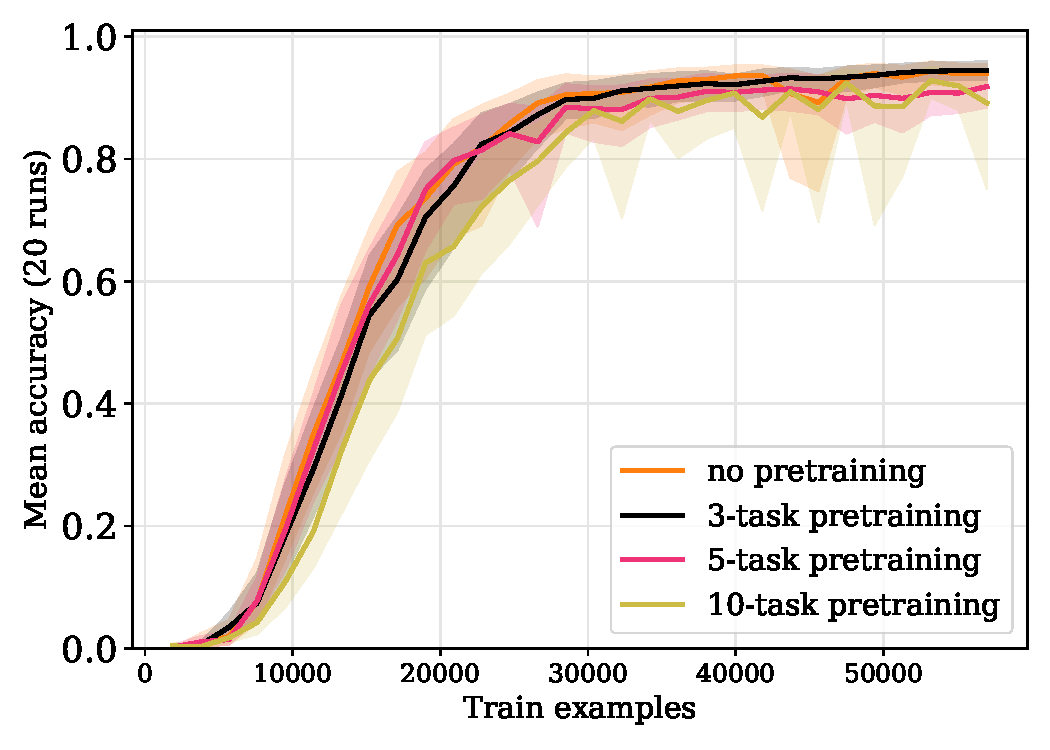
\includegraphics[width=1\linewidth]{../fig/fuzzy-lm-pretrain-compare-train_size-pretrained-embed_dim=None.pdf}
 \caption{Results where random representations are grounded via pretraining learning tasks. Simulations adopt the best-performing settings from the no-pretraining condition (2-dimensional embeddings, 100-dimensional hidden representations).}
 \label{fig:fuzzy-lm-pretrain-results}
\end{subfigure}
\caption{Sequential same--different results with and without pretraining.}
\end{figure*}

\subsection{Discussion}

These sequential models are given no negative examples and they must predict into a totally new vocabulary. Despite these challenges, they succeed at learning the underlying patterns in our data, even though they use only random representations. On the other hand, the learning process is slow and data-intensive. We hypothesized that grounding representations in property domains via pretraining might lead to noticeable speed-ups, as it did in \secref{sec:equality}, but we did not see this effect in practice. We speculate that there may be model variants that reduce these demands, given that learning is in principle possible in this architecture, but we did not discover them and leave them to future work.

\section{Model 3: Hierarchical same--different relations}\label{sec:premack}

Given the strong results found for simple equality relations in \secref{sec:equality}, we can ask whether more challenging equality problems are also learnable in our setting. The hierarchical equality task used by \citet{Premack:1983} is an interesting test case: given a pairs of pairs $((a,b), (c,d))$, the label is $1$ if $(a = b) = (c = d)$, else $0$. \citet{Premack:1983} suggested that the ability exemplified by this task -- reasoning about hierarchical \emph{same} and \emph{different} relations -- could represent a form of symbolic abstraction uniquely enabled by language. Given the non-symbolic nature of our models, our simulations provide a test of this hypothesis, though we should look critically at their ability to find good solutions with reasonable amounts of training data.

\subsection{Model}

We can approach this task using the same model and methods as we used for equality. The only change required to equations \dasheg{eq:x2h}{eq:h2y} is that we create inputs $[a;b;c;d]$: the flat concatenation of all the elements of the two pair of vectors. This change in turn leads $W_{xh}$ to have dimensionality $4m \times n$.

These models are able to find nearly perfect solutions, but vastly more training data is required for this task than was required for simple equality, and the network configuration matters much more. For example, our model with 10-dimensional entity representations and 100-dimensional hidden representations reached near perfect accuracy, but only with over 95,000 training instances. A comparable model with 50-dimensional entity representations failed to get traction at all with this amount of training data, and pretraining led to only minor improvements. \Appref{app:model1-premack} provides a full picture of these learning trends.

% MCF: I was confused about the numbers in the paragraph above compared with the graph. it looks like we're graphing examples, not epochs, but 95k is not necessary for any of the architectures shown...

We hypothesized that the flat input representations $[a;b;c;d]$ might be suboptimal here. This task is intuitively hierarchical: if one works out the equality labels for each of the two pairs, then the further classification decision can be done entirely on that basis. Our current neural network might be too shallow to find this kind of decomposition. To address this, we can simply add another intermediate layer:
%
\begin{align}
h_{1} &= \ReLU([a;b;c;d]W_{xh} + b_{h_{1}}) \label{eq:x2h1}\\
h_{2} &= \ReLU(h_{1}W_{hh} + b_{h_{2}}) \label{eq:x2h2}\\
y &= \softmax(h_{2}W_{hy} + b_{y}) \label{eq:h2y2}
\end{align}


\subsection{Results}

\Figref{fig:premack-h2-flat-results} shows that these deeper networks learn faster and are more robust to different network configurations than the single-layer variant. Intuitively, these models are better structured to find hierarchical solutions to this hierarchical problem. Pretraining led to further gains in training speed (\figref{fig:premack-h2-pretrain}).

\begin{figure*}[tp]
\centering
\begin{subfigure}[t]{0.48\linewidth}
 \centering
 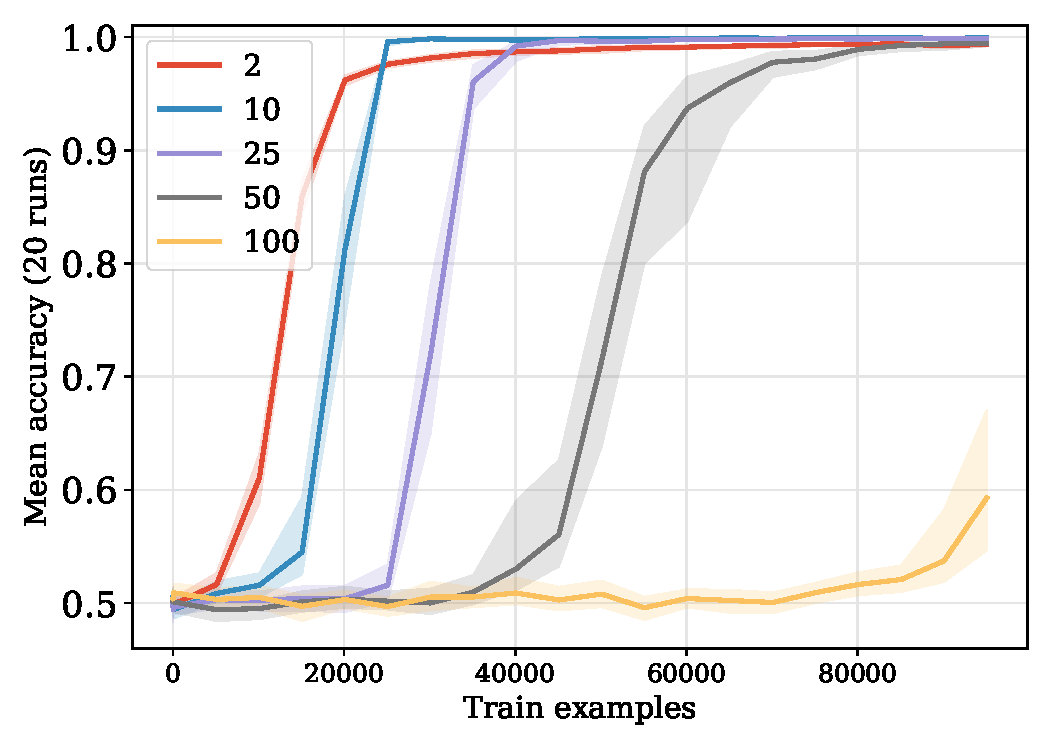
\includegraphics[width=1\linewidth]{../fig/flatpremack-h2-train_size-embed_dim-hidden_dim=100.pdf}
 \caption{Results for a network with two 100-dimensional hidden layers. Nearly all the networks solve the task, but they require very large training sets to do so.}
 \label{fig:premack-h2-flat-results}
\end{subfigure}
\hfill
\begin{subfigure}[t]{0.48\linewidth}
 \centering
 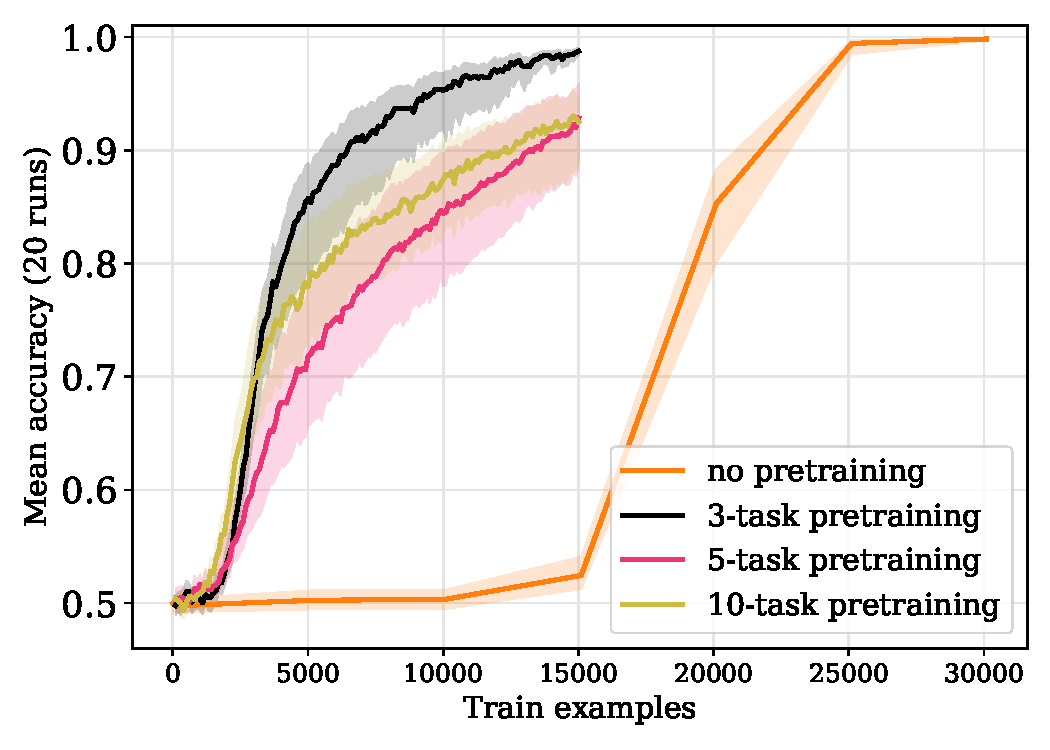
\includegraphics[width=1\linewidth]{../fig/flatpremack-h2-pretrain-compare-train_size-pretrained-embed_dim=None.pdf}
 \caption{Results from pre-trained networks, adopting the best of the models at left (10-dimensional embeddings, 100-dimensional hidden representations).}
 \label{fig:premack-h2-pretrain}
\end{subfigure}
\caption{Hierarchical same--different results with and without pretraining.}
\end{figure*}


\subsection{Discussion}

These results are encouraging, but we still require more than 20,000 training instances to reach top performance and upwards of 10,000 examples even with pretraining. This amount is still vastly more data than human participants get in similar experiments, which typically involve short exposures in the range of dozens to hundreds of examples \cite[e.g.,][]{marcus:1999,endress2005}. Thus, it is worth asking whether there are other solutions that would be more data efficient and more in line with human capabilities. We next sought to capitalize even more on the hierarchical nature of this task by defining a modular pretraining regime in which previously learned capabilities are recruited for new tasks.

\subsection{The critical role of experience}\label{sec:modular}

Our successful results training neural networks on simple equality suggested another strategy for solving the hierarchical equality task. Rather than requiring our networks to find solutions from scratch, we pretrained them on basic equality tasks and then used those parameters as a starting point for learning hierarchical equality. This set of simulations was conceptually similar to our previous experiments with pretraining, but now we pretrained an entire subpart of the model, rather than just input representations.

\subsubsection{Model}

The hierarchical equality task requires computing the equality relation three times: compute whether the first two inputs are equal, compute whether the second two inputs are equal, then compute whether the truth-valued outputs of these first two computations are equal. We propose to use the same network pretrained on basic equality to perform all three equality computations. More precisely, we define
%
\begin{align}
h_1 &= \ReLU([a;b]W_{xh} + b_{h})\\
h_2 &= \ReLU([c;d]W_{xh} + b_{h})\\
h_3 &= \ReLU([h_1;h_2]W_{xh} + b_{h}) \\
y &= \softmax(h_3W_{hy} + b_{y})
\end{align}
%
where $W_{xh}$, $W_{hy}$, $b_h$, and $b_y$ are the parameters from the model in equations \dasheg{eq:x2h}{eq:h2y} already trained on basic equality. Crucially, the same parameters, $W_{xh}$ and $b_h$, are used three times: twice to compute representations encoding whether a pair of input entities are equal ($h_1$, $h_2$), and once to compute a representation ($h_{3}$) encoding whether the truth values encoded by $h_1$ and $h_2$ are equal. This final representation is then used to compute a probability distribution over two classes, and the class with the higher probability is predicted by the model.

\begin{figure*}[tp]
\centering
\begin{subfigure}[t]{0.48\textwidth}
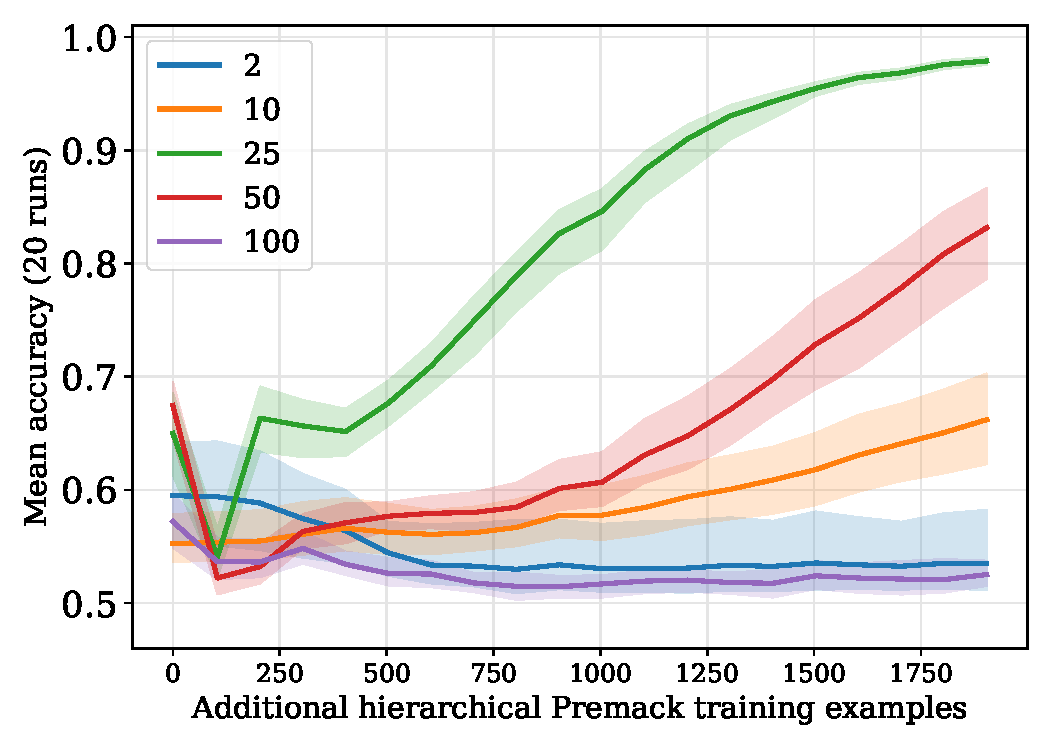
\includegraphics[width=1\linewidth]{../fig/input-as-output-train_size-embed_dim-hidden_dim=0.pdf}
\caption{Basic equality networks applied to the hierarchical equality task. Each line represents a different embedding dimensionality, which is constrained in this model to match the hidden dimensionality. Even with no additional training instances for this task, all models achieve greater than chance accuracy, and even modest amounts of additional training on the task lead to excellent performance.
}
\label{fig:premack-pretraining-results}
\end{subfigure}
\hfill
\begin{subfigure}[t]{0.48\textwidth}
 \centering
 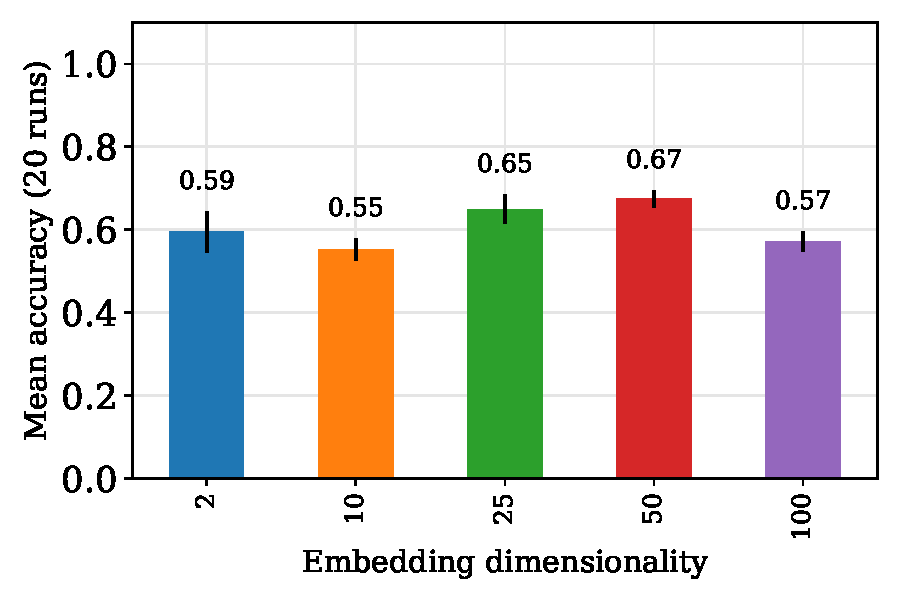
\includegraphics[width=1\linewidth]{../fig/input-as-output-zero-shot.pdf}
 \caption{\update{The results from the plot at left where the x-axis is 0, that is, where we are testing zero-shot generalization from the pretrained equality network to the hierarchical setting. All the models perform well above chance in this setting, with the 50-dimensional version achieving a mean of 67\% accuracy.}}
 \label{fig:premack-pretraining-zero-shot-results}
\end{subfigure}
\caption{Modular network results for the hierarchical same--different task.}
\label{fig:modular-results}
\end{figure*}

\subsubsection{Results and discussion}

\Figref{fig:modular-results} shows that this model succeeds very quickly at the hierarchical equality task. As we see in \figref{fig:premack-pretraining-results}, after just a few thousand examples, the majority of the model configurations perform with near perfect accuracy. The findings in \figref{fig:premack-pretraining-zero-shot-results} are even more striking: all the models have above chance performance after being trained only on the simple equality task -- that is, they achieve zero-shot generalization to the hierarchical task. It is remarkable that a model trained only on equality between entities is able to get traction on a problem that requires determining whether equality holds between the truth values encoded in two learned representations.

It might be possible to effectively combine network pretraining with input pretraining as in the previous experiments. An initial exploration of this idea is presented in \appref{app:double-pretrain}. While we have not yet found a way to use this combination of pretraining regimes to improve over \figref{fig:modular-results}, we are optimistic about such combinations for future work.

\section{General Discussion}

Equality is a key case study for understanding the origins of human relational reasoning. This case study has been puzzling for symbolic accounts of reasoning because such accounts do not provide a compelling explanation for why some equality tasks are so easy to learn and others are so hard. In addition, evidence of graded learning and generalization in non-human species suggests that a gradual learning account might provide more traction in explaining the empirical data \cite{wasserman:2017}. Inspired by this work, we revisited a long-standing debate about whether neural network models can learn equality relations from data \cite{alhama:2019}. We presented a series of such models that succeeded even in stringent assessments, and, in the case of neural language models, even without being shown negative examples.
% We further supported these results with analytic insights into why networks are able to find solutions to these tasks.

In some settings, our current models require more training instances than humans seem to need. However, our pretraining approach suggests a path forward: by using pretrained models as modular components, we can get traction on challenging tasks without any training specifically for those tasks. In some cases, even a small amount of additional training can make a substantial difference. Perhaps modular, pretrained components could serve as the basis for more complex cognitive abilities more generally.

One implication of these pretraining findings is that it should be possible to scaffold performance in complex, hierarchical equality tasks via training on simpler ones. Indeed, \citet{smirnova2015} show just this result in crows, consistent with our findings. Although we do not discount the potential role of linguistic labels in informing adult humans' expertise in such tasks \cite{gentner2003}, pretraining also provides a potential account of how infants and young children might succeed in a range of equality reasoning tasks without access to specific linguistic symbols like ``same'' \cite{walker:2016,ferry:2015,hochmann2016}.

More broadly still, our work suggests a possible way forward in understanding the acquisition of logical semantics. Graded logical functions like those our models learned here could form the foundation for a semantics of words like ``same'' \cite{potts2019}. Such an option is appealing because it escapes from the circularity of defining the semantics of linguistic symbols as originating in a mental primitive {\sc same}. A semantics for ``same'' requires defining its inputs and outputs as well as how it composes with other symbols. The assertion that there is a primitive identity computation does not provide these; it further fails to explain the flexibility that allows us to call two Toyota Corollas ``the same'' but two twin sisters ``different.'' In contrast, the kinds of networks we propose here could in principle be conditioned contextually to provide flexible, context-sensitive interpretation of logical meaning. % MCF: could we cite some of Ruben's work or the natural language inference work here maybe? or is there something more appropriate?

Earlier debates about the nature of equality computations centered around the question of whether models included symbolic elements. We believe ours do not; but it is of course possible to quibble with this judgment. For example, since the supervisory signal used in Models 1 and 3 is generated based on a symbolic rule, perhaps that makes these models symbolic under some definition. (Of course, the same argument could be applied to the supervision signal that is provided to crows, baboons, and human children). We view this kind of argument as terminological, rather than substantive. In the end, our goal is an explicit learning theory for relational reasoning. Our hope is that the work described here takes a first step in this direction.

% The claim that certain forms of representation are equivalent to including symbolic primitives is untroubling if these representations enhance the generalization skills of neural models; some class of neural models might be labeled as symbolic, but that does not nullify the fact that they are successful models of graded relational learning and distinct from uncontroversially symbolic models \cite[e.g.,][]{frank:2011}.


% BACK TO SYMBOLIC, LANGUAGE, SEMANTICS

% the debate has been whether there is a symbol. We view this as the least important issue. A single ``same" symbol cannot account for the vast range of behaviors that we want to explain -- how are two toyota corollas the same, while two people are not?
% To be an explanatory account, a symbol needs a semantics - what are the inputs, outputs, how does it compose. Without these, there is no account of behavior.

% same isn't a relation, it's a set of possible relations


% you can think of it this way: our networks are a semantics for the symbol

% This is maybe unfamiliar, because you might think you'd do this in a logical language or have an axiom system, but our networks are perfect and so you'd never notice. MARR cite



% We report results with and without pretraining. While \citeauthor{marcus:2001} might consider our pretraining method to be symbolic, we believe it would be difficult to argue that random distributed representations are symbolic, as they do not encode any properties directly. We additionally believe that the symbolic/non-symbolic distinction does not provide an explanation for the state of the comparative and developmental literature on relational learning, as we will argue in \secref{sec:?}.}

% SYMBOLIC VS. NON-Symbolic
% - this distinction doesn't helps
% - neural models clearly different
% - supervision unclear
% - not helpful (localist could be symbolic & unstructured)
%
% Since the initial debate, neural networks have become

%Finally, we note that, while the pretrained representations in \figref{fig:reps:pretrained} encode property values via linear structures, this is only because we used linear classifiers in our pretraining tasks. There are a practically limitless number of different ways to encode property values via abstract structures.

 % By contrast, the literature on relational learning in neural networks is currently limited to feature representations, and does not consider any non-featural representations where property values are encoded implicitly with abstract structures. For example, all of the experiments reviewed in \cite{alhama:2019} use feature representations, meaning that each vector unit explicitly contains the value of a property. Their negative conclusions about relational learning in neural networks hold only for networks using such representations.


\ifthenelse{
  \equal{\papermode}{pnas}
}{
  \matmethods{The code and data used to run the experiments in this paper are publicly available at: https://github.com/atticusg/NeuralRelationalReasoning.}

%\subsection*{Subsection for Method}
%Example text for subsection.
%}

\showmatmethods{} % Display the Materials and Methods section

\acknow{This work is supported in part by a Facebook Robust Deep Learning for Natural Language Processing Research Award and by the McDonnell Foundation grant ``The Nature and Origins of the Human Capacity for Abstract Combinatorial Thought''.}

\showacknow{} % Display the acknowledgments section

% Bibliography
\bibliography{relational-learning-bib}

%\documentclass[9pt,twoside,lineno]{pnas-new}
% Use the lineno option to display guide line numbers if required.

\templatetype{pnassupportinginfo}

\title{Your main manuscript title}
\author{Author1, Author2 and Author3 (complete author list)}
\correspondingauthor{Corresponding Author name.\\E-mail: author.two@email.com}

\input{pre-macros}


\begin{document}

\maketitle

%% Adds the main heading for the SI text. Comment out this line if you do not have any supporting information text.
\SItext


% \appendix

\section{Model 1 Supplementary Methods}

The input to our model is a pair of vectors $(a, b)$, each of dimension $m$, which correspond to the two stimulus objects. These vectors are non-featural representations that do not have features encoding properties of the objects or their identity. These are concatenated to form a single vector $[a;b]$ of dimension $2m$, which is the simplest way of merging the two representations to form a single input.

This representation is multiplied by a matrix of weights $W_{xh}$ of dimension $2m \times n$ and a bias vector $b_{h}$ of dimension $n$ is added to this result, where $n$ is the hidden layer dimensionality. These two steps create a linear projection of the input representation, and the bias term is the value of this linear projection when the input representation is the zero vector. Then, the non-linear activation function $\ReLU$ ($\ReLU(x) = \max(0, x)$) is applied element-wise to this linear projection. This non-linearity is what gives the neural model more expressive power than a logistic regression \citep{Cybenko:1989,Hornik:Stinchcombe:White:1989}. The result is the hidden representation $h$.

The hidden representation is the input to the classification layer: $h$ is multiplied by a second matrix of weights $W_{hy}$, dimension $n \times 2$, and a bias term $b_{y}$ (dimension 2) is added to this. This second bias term encodes the probabilities of each class when the hidden representation is 0. The result is fed through the softmax activation function: $\softmax(x)_{i} = \frac{\exp{x_{i}}}{\sum_{j} \exp{x_{j}}}$. This creates a probability distribution over the classes (positive and negative). For a given input, the model computes this probability distribution and the input is categorized as the class with the higher probability.

During training, this model is presented with positive and negative labeled examples and the parameters $W_{xh}$, $W_{hy}$, $b_{y}$, and $b_{h}$ are learned using back propagation with a cross entropy function. \update{This function is defined as follows, for a set of $N$ examples and $K$ classes:
%
\begin{equation}
\max(\theta)
\quad
\frac{1}{N}
\sum_{i=1}^{N}
\sum_{k=1}^{K}
y^{i,k} \log(h_{\theta}(i)^{k})
\end{equation}
%
where $\theta$ abbreviates the model parameters ($W_{xh}$, $W_{hy}$, $b_{y}$, $b_{h}$), $y^{i,k}$ is the actual label for example $i$ and class $k$, and $h_{\theta}(i)^{k}$ is the corresponding prediction.}


\section{Model 2 Supplementary Methods}

The input to this model is a sequence of vectors $x_1, x_2, x_3, \dots$, each of dimension $m$, which correspond to a sequence of stimulus objects. These vectors are, again, non-featural representations that do not have features encoding properties of the objects or their identity.


At each timestep $t$, the input vector $x_t$ is fed into the $\LSTM$ cell along with the previous hidden representation $h_{t-1}$. The defining feature of an $\LSTM$ is the ability to decide whether to store information from the current input, $x_t$, and whether to remember or forget the information from the previous timestep $h_{t-t}$. The output of the $\LSTM$ cell is the hidden representation for the current time step $h_t$. The dimension of the hidden representations is $n$. The hidden representation is multiplied by a matrix $W$ with dimensionality $n \times m$ to produce $y_t$. This result, $y_t$, is a linear projection of the hidden representation into the input vector space, which is necessary because $y_t$ is a prediction of what the next input, $x_{t+1}$, will be.

% \update{
The objective function is as follows:
%
\begin{equation}
\max(\theta)
\quad
-\frac{1}{N}
\sum_{i=1}^{N}
\sum_{t=1}^{T_{i}}
\left\| h_{\theta}\left(x^{i, 0:{t-1}}\right) - x^{i,t} \right\|^{2}
\end{equation}
%
for $N$ examples. Here, $T_{i}$ is the length of example $i$. As before, $\theta$ abbreviates the parameters of the model as specified in \dasheg{eq:lstm-recur}{eq:lstm-predict}. We use $h_{\theta}(x^{i, 0:{t-1}})$ for the vector predicted by the model for example~$i$ at timestep~$t$, which is compared to the actual vector at timestep $t$ via squared Euclidean distance (i.e., the mean squared error).
% As noted above, this is an unusual formulation for a language model. The usual version essentially treats every timestep as involving a classification decision, with a cross-entropy loss. We cannot adopt this because of our goal of using unseen vocabulary items at test time. % MCF: seemed redundant


\section{Model figures}


\subsection{Model 1: Same--different relation with feed-foward  networks}\label{sec:model1}

Our model of equality is given by \dasheg{eq:x2h-supp}{eq:h2y-supp}:
%
\begin{align}
  h &= \ReLU([a;b]W_{xh} + b_{h}) \label{eq:x2h-supp}\\
  y &= \softmax(hW_{hy} + b_{y}) \label{eq:h2y-supp}
\end{align}
%
The input is a pair of vectors $(a,b)$, each of dimension $m$, which correspond to two stimulus objects. These vectors are non-featural representations that do not hav efeatures encoding properties of the objects or their identities. These are concatenated to form a single vector $[a;b]$ of dimension $2m$, which is the simplest way of merging the two representations to form a single input.

This representation is multiplied by a matrix of weights $W_{xh}$ of dimension $2m \times n$ and a bias vector $b_{h}$ of dimension $n$ is added to this result, where $n$ is the hidden layer dimensionality. These two steps create a linear projection of the input representation, and the bias term is the value of this linear projection when the input representation is the zero vector. Then, the non-linear activation function $\ReLU$ ($\ReLU(x) = \max(0, x)$) is applied element-wise to this linear projection. This non-linearity is what gives the neural model more expressive power than a logistic regression \citep{Cybenko:1989,Hornik:Stinchcombe:White:1989}. The result is the hidden representation $h$.

The hidden representation is the input to the classification layer: $h$ is multiplied by a second matrix of weights $W_{hy}$, dimension $n \times 2$, and a bias term $b_{y}$ (dimension 2) is added to this. This second bias term encodes the probabilities of each class when the hidden representation is 0. The result is fed through the softmax activation function: $\softmax(x)_{i} = \frac{\exp{x_{i}}}{\sum_{j} \exp{x_{j}}}$. This creates a probability distribution over the classes (positive and negative). For a given input, the model computes this probability distribution and the input is categorized as the class with the higher probability.

The parameters $W_{xh}$, $W_{hy}$, $b_{y}$, and $b_{h}$ are learned using back propagation with a cross entropy function. \update{This function is defined as follows, for a set of $N$ examples and $K$ classes:
%
\begin{equation}\label{eq:crossent}
\max(\theta)
\quad
\frac{1}{N}
\sum_{i=1}^{N}
\sum_{k=1}^{K}
y^{i,k} \log(h_{\theta}(i)^{k})
\end{equation}
%
where $\theta$ abbreviates the model parameters ($W_{xh}$, $W_{hy}$, $b_{y}$, $b_{h}$), $y^{i,k}$ is the actual label for example $i$ and class $k$, and $h_{\theta}(i)^{k}$ is the corresponding prediction.}

\Figref{fig:models:equality} provides a visual depiction of the model. The gray boxes correspond to embedding representations, the purple box is the hidden representation $h$, and the red box is the output distribution $y$. Dotted arrows depict concatenation, and solid arrows depict the dense relations corresponding to the matrix multiplications (plus bias terms) in \dasheg{eq:x2h}{eq:h2y}.

\begin{figure}[H]
  \centering
  \resizebox{100pt}{!}{%
    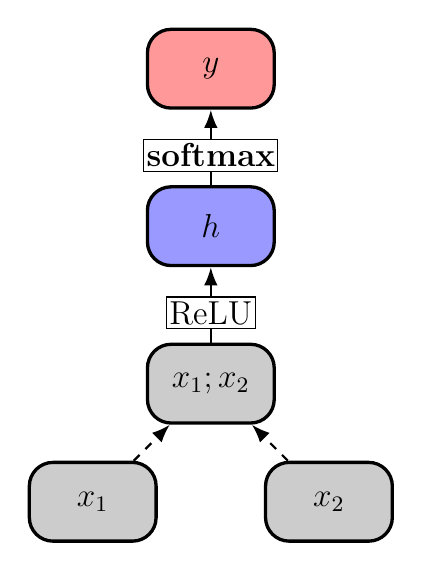
\begin{tikzpicture}[
      % GLOBAL CFG
      font=\sf \large,
      >=LaTeX,
      % Styles
      rep/.style={% For representations
        rectangle,
        rounded corners=3mm,
        draw,
        very thick,
        minimum height =1cm,
        minimum width=1.61cm
      },
      function/.style={%For functions
        ellipse,
        draw,
        inner sep=1pt
      },
      gt/.style={% For internal inputs
        rectangle,
        draw,
        minimum width=5mm,
        minimum height=4mm,
        inner sep=1pt
      },
      function/.style={
        rectangle,
        draw,
        minimum width=5mm,
        minimum height=4mm,
        inner sep=1pt
      },
      arrowconcat/.style={% Arrows for concatenation
        rounded corners=.25cm,
        dashed,
        thick,
        ->,
      },
      arrowfunction/.style={% Arrows for concatenation
        rounded corners=.25cm,
        thick,
        ->,
      }
      ]

      % Start drawing the thing...
      % Draw the cell:
      \node [rep, fill=\inputcolor] (input1) at (-1.5,1.5){$x_1$} ;
      \node [rep, fill=\inputcolor] (input2) at (1.5,1.5){$x_2$} ;
      \node [rep, fill=\inputcolor] (concat) at (0,3){$x_1;x_2$} ;
      \draw [arrowconcat] (input1) -- (concat);
      \draw [arrowconcat] (input2) -- (concat);


      \node [rep, fill=\hiddencolor] (hidden) at (0,5){$h$} ;
      \node [gt, minimum width=1cm] (relu) at (0,4-0.1) {$\ReLU$};
      \draw [arrowfunction] (concat) -- (relu) -- (hidden);


      \node [rep,fill=\outputcolor] (output) at (0,7){$y$} ;
      \node [gt, minimum width=1cm] (softmax) at (0,6-0.1) {$\softmax$};
      \draw [arrowfunction] (hidden) -- (softmax) -- (output);

    \end{tikzpicture}
  }
  \caption{A single layer network computing equality.}
  \label{fig:models:equality}
\end{figure}


\subsection{Model 2: Sequential same--different (ABA task)}\label{sec:model2}

The specific model we use for this is as follows:
%
\begin{align}
  h_{t} &= \LSTM(x_{t}, h_{t-1}) \label{eq:lstm-recur-supp}\\
  y_{t} &= h_{t}W + b\label{eq:lstm-predict-supp}
\end{align}
%
This holds for $t > 0$, and we set $h_{0} = \mathbf{0}$. $\LSTM$ is a long short-term memory cell \cite{hochreiter:1997}. Full details on these cells are given in \appref{sec:analyticlm}.

The input is a sequence of vectors $x_1, x_2, x_3, \dots$, each of dimension $m$, which correspond to a sequence of stimulus objects. These vectors are, again, non-featural representations that do not have features encoding properties of the objects or their identity.

At each timestep $t$, the input vector $x_t$ is fed into the $\LSTM$ cell along with the previous hidden representation $h_{t-1}$. The defining feature of an $\LSTM$ is the ability to decide whether to store information from the current input, $x_t$, and whether to remember or forget the information from the previous timestep $h_{t-t}$. The output of the $\LSTM$ cell is the hidden representation for the current time step $h_t$. The dimension of the hidden representations is $n$. The hidden representation is multiplied by a matrix $W$ with dimensionality $n \times m$ to produce $y_t$. This result, $y_t$, is a linear projection of the hidden representation into the input vector space, which is necessary because $y_t$ is a prediction of what the next input, $x_{t+1}$, will be.

The objective function is as follows:
%
\begin{equation}
\max(\theta)
\quad
-\frac{1}{N}
\sum_{i=1}^{N}
\sum_{t=1}^{T_{i}}
\left\| h_{\theta}\left(x^{i, 0:{t-1}}\right) - x^{i,t} \right\|^{2}
\end{equation}
%
for $N$ examples. Here, $T_{i}$ is the length of example $i$. As before, $\theta$ abbreviates the parameters of the model as specified in \dasheg{eq:lstm-recur-supp}{eq:lstm-predict-supp}. We use $h_{\theta}(x^{i, 0:{t-1}})$ for the vector predicted by the model for example~$i$ at timestep~$t$, which is compared to the actual vector at timestep $t$ via squared Euclidean distance (i.e., the mean squared error).

\Figref{fig:reps:sequence} depicts this model. At each timestep $t$, a vector $y_{t}$ (red) is predicted based on the input representation at $t$ (gray) and the hidden representation at $t$ (purple). During training, this is compared with the actual vector for timestep $t+1$ (green). During testing, the predicted vector $y_{i}$ is compared with every item in the union of the train and assessment vocabularies, and the closest vector (according to Euclidean distance) is taken to be the prediction. This vector is then used as the input for timestep $t+1$.

\begin{figure}[H]
  \centering
  \resizebox{240pt}{!}{%
    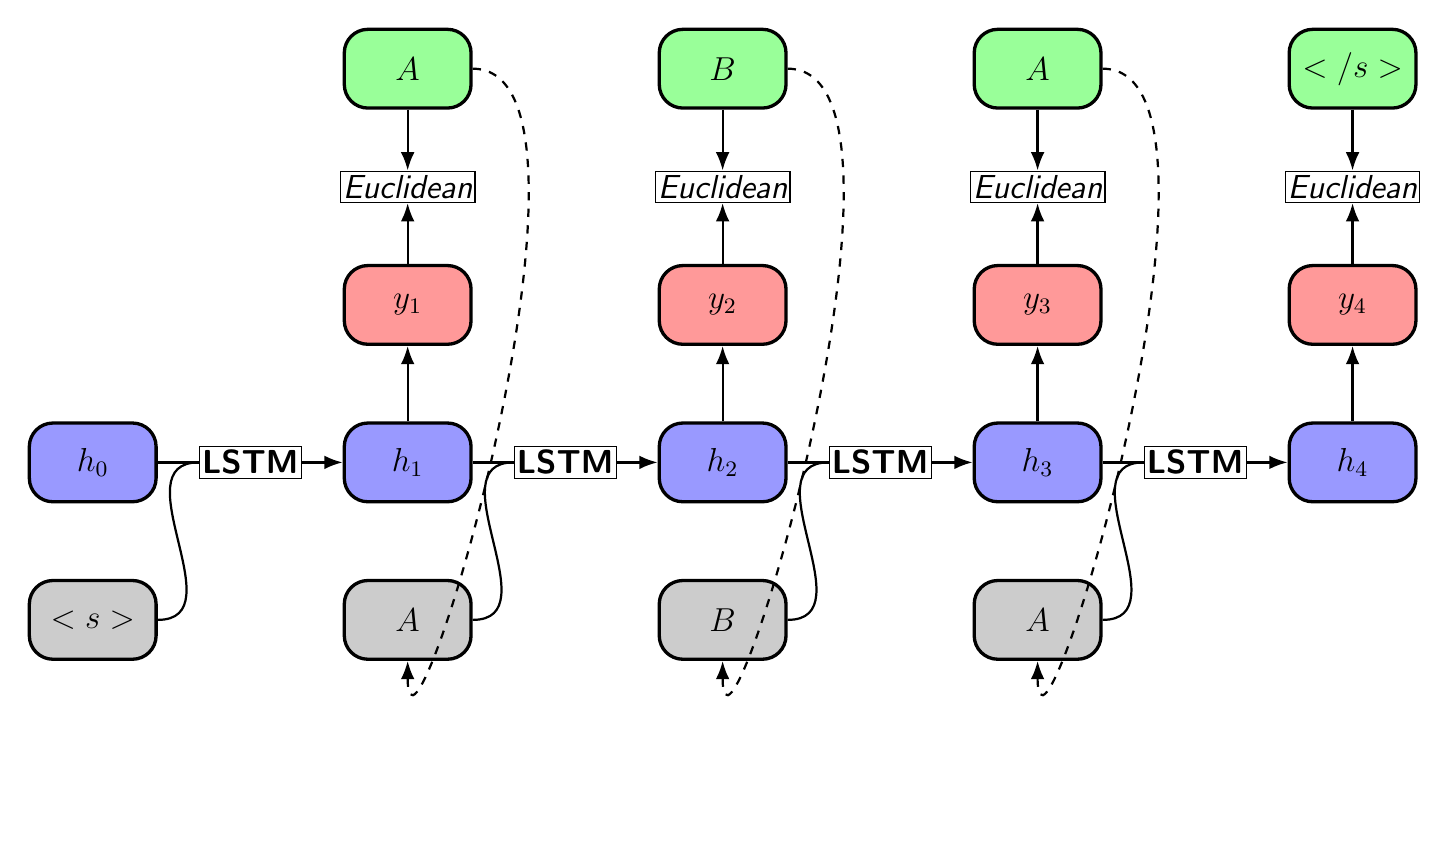
\begin{tikzpicture}[
      % GLOBAL CFG
      font=\sf \large,
      >=LaTeX,
      % Styles
      rep/.style={% For representations
        rectangle,
        rounded corners=3mm,
        draw,
        very thick,
        minimum height =1cm,
        minimum width=1.61cm
      },
      function/.style={%For functions
        ellipse,
        draw,
        inner sep=1pt
      },
      gt/.style={% For internal inputs
        rectangle,
        draw,
        minimum width=5mm,
        minimum height=4mm,
        inner sep=1pt
      },
      function/.style={
        rectangle,
        draw,
        minimum width=5mm,
        minimum height=4mm,
        inner sep=1pt
      },
      arrowconcat/.style={% Arrows for concatenation
        rounded corners=.25cm,
        dashed,
        thick,
        ->,
      },
      arrowfunction/.style={% Arrows for concatenation
        rounded corners=.25cm,
        thick,
        ->,
      }
      ]

      % Start drawing the thing...
      % Draw the cell:
      \node [rep, fill=\inputcolor] (input1) at (-10,4){$<s>$} ;
      \node [rep, fill=\inputcolor] (input2) at (-6,4){$A$} ;
      \node [rep, fill=\inputcolor] (input3) at (-2,4){$B$} ;
      \node [rep, fill=\inputcolor] (input4) at (2,4){$A$} ;

      \node [rep, fill=\hiddencolor] (hidden0) at (-10,6){$h_0$} ;
      \node [rep, fill=\hiddencolor] (hidden1) at (-6,6){$h_1$} ;
      \node [rep, fill=\hiddencolor] (hidden2) at (-2,6){$h_2$} ;
      \node [rep, fill=\hiddencolor] (hidden3) at (2,6){$h_3$} ;
      \node [rep, fill=\hiddencolor] (hidden4) at (6,6){$h_4$} ;

      \node [gt] (LSTM0) at (-8,6){$\LSTM$} ;
      \node [gt] (LSTM1) at (-4,6){$\LSTM$} ;
      \node [gt] (LSTM2) at (0,6){$\LSTM$} ;
      \node [gt] (LSTM3) at (4,6){$\LSTM$} ;

      \node [rep, fill=\outputcolor] (output1) at (-6,8){$y_1$} ;
      \node [rep, fill=\outputcolor] (output2) at (-2,8){$y_2$} ;
      \node [rep, fill=\outputcolor] (output3) at (2,8){$y_3$} ;
      \node [rep, fill=\outputcolor] (output4) at (6,8){$y_4$} ;

      \node [gt] (compare1) at (-6,9.5){$\compare$} ;
      \node [gt] (compare2) at (-2,9.5){$\compare$} ;
      \node [gt] (compare3) at (2,9.5){$\compare$} ;
      \node [gt] (compare4) at (6,9.5){$\compare$} ;

      \node [rep, fill=\colorlabel] (label1) at (-6,11){$A$} ;
      \node [rep, fill=\colorlabel] (label2) at (-2,11){$B$} ;
      \node [rep, fill=\colorlabel] (label3) at (2,11){$A$} ;
      \node [rep, fill=\colorlabel] (label4) at (6,11){$</s>$} ;

      \draw [arrowfunction] (label1) -- (compare1);
      \draw [arrowfunction] (label2) -- (compare2);
      \draw [arrowfunction] (label3) -- (compare3);
      \draw [arrowfunction] (label4) -- (compare4);

      \draw [arrowfunction] (output1) -- (compare1);
      \draw [arrowfunction] (output2) -- (compare2);
      \draw [arrowfunction] (output3) -- (compare3);
      \draw [arrowfunction] (output4) -- (compare4);

      \draw [arrowfunction] (hidden1) -- (output1);
      \draw [arrowfunction] (hidden2) -- (output2);
      \draw [arrowfunction] (hidden3) -- (output3);
      \draw [arrowfunction] (hidden4) -- (output4);

      \draw [thick] (input1) to[out=0,in=-180, distance=1cm] (LSTM0);
      \draw [thick] (input2) to[out=0,in=-180, distance=1cm] (LSTM1);
      \draw [thick] (input3) to[out=0,in=-180, distance=1cm] (LSTM2);
      \draw [thick] (input4) to[out=0,in=-180, distance=1cm] (LSTM3);

      \draw [arrowfunction] (hidden0) -- (LSTM0) -- (hidden1);
      \draw [arrowfunction] (hidden1) -- (LSTM1)-- (hidden2);
      \draw [arrowfunction] (hidden2) -- (LSTM2)-- (hidden3);
      \draw [arrowfunction] (hidden3) -- (LSTM3)-- (hidden4);

      \draw[->,dashed,thick] (label1) to[out=0,in=-90, distance=1.99cm] (input2);
      \draw[->,dashed,thick] (label2) to[out=0,in=-90, distance=1.99cm] (input3);
      \draw[->,dashed,thick] (label3) to[out=0,in=-90, distance=1.99cm] (input4);
    \end{tikzpicture}
  }
  \caption{A recursive LSTM network producing ABA sequences.}
  \label{fig:reps:sequence}
\end{figure}

\subsection{Model 3a: A single layer feed forward network }
 The only change required to equations \dasheg{eq:x2h-supp}{eq:h2y-supp} is that we create inputs $[a;b;c;d]$: the flat concatenation of all the elements of the two pair of vectors. This change in turn leads $W_{xh}$ to have dimensionality $4m \times n$. The objective function is again defined using a cross entropy function, as in equation \ref{eq:crossent}. \Appref{app:model1-premack} provides a full picture of these learning trends. These models are able to find nearly perfect solutions, but vastly more training data is required for this task than was required for simple equality, and the network configuration matters much more. For example, our model with 10-dimensional entity representations and 100-dimensional hidden representations reached near perfect accuracy, but only with over 95,000 training instances. A comparable model with 50-dimensional entity representations failed to get traction at all with this amount of training data, and pretraining led to only minor improvements. For this reason, we also perform experiments with a deeper neural network.


\subsection{Model 3b: A deeper feed-forward network for hierarchical same--different}\label{sec:model3a}

This model extends \dasheg{eq:x2h-supp}{eq:h2y-supp} with an additional hidden layer and a larger input dimensionality, corresponding to the input pair of pairs $((a,b), (c,d))$ being flattened into a single concatenated representation $[a;b;c;d]$:
%
\begin{align}
  h_{1} &= \ReLU([a;b;c;d]W_{xh} + b_{h_{1}}) \label{eq:x2h1-supp}\\
  h_{2} &= \ReLU(h_{1}W_{hh} + b_{h_{2}}) \label{eq:x2h2-supp}\\
  y &= \softmax(h_{2}W_{hy} + b_{y}) \label{eq:h2y2-supp}
\end{align}
%
The objective function is again defined using a cross entropy function, as in equation \ref{eq:crossent}.

\Figref{fig:models:premack-deep} depicts this model.

\begin{figure}[H]
  \centering
  \resizebox{150pt}{!}{%
    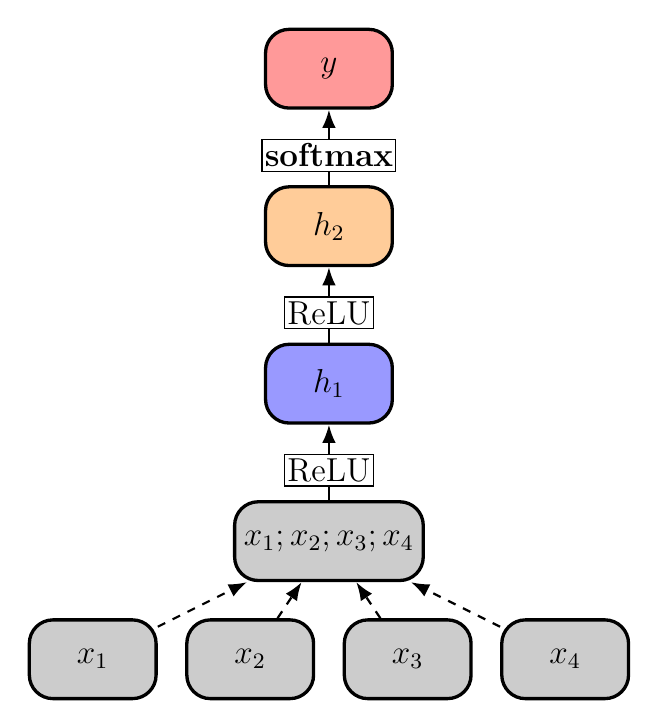
\begin{tikzpicture}[
      % GLOBAL CFG
      font=\sf \large,
      >=LaTeX,
      % Styles
      rep/.style={% For representations
        rectangle,
        rounded corners=3mm,
        draw,
        very thick,
        minimum height =1cm,
        minimum width=1.61cm
      },
      function/.style={%For functions
        ellipse,
        draw,
        inner sep=1pt
      },
      gt/.style={% For internal inputs
        rectangle,
        draw,
        minimum width=5mm,
        minimum height=4mm,
        inner sep=1pt
      },
      function/.style={
        rectangle,
        draw,
        minimum width=5mm,
        minimum height=4mm,
        inner sep=1pt
      },
      arrowconcat/.style={% Arrows for concatenation
        rounded corners=.25cm,
        dashed,
        thick,
        ->,
      },
      arrowfunction/.style={% Arrows for concatenation
        rounded corners=.25cm,
        thick,
        ->,
      }
      ]

      % Start drawing the thing...
      % Draw the cell:
      \node [rep, fill=\inputcolor] (input1) at (-3,1.5){$x_1$} ;
      \node [rep, fill=\inputcolor] (input2) at (-1,1.5){$x_2$} ;
      \node [rep, fill=\inputcolor] (input3) at (1,1.5){$x_3$} ;
      \node [rep, fill=\inputcolor] (input4) at (3,1.5){$x_4$} ;
      \node [rep, fill=\inputcolor] (concat) at (0,3){$x_1;x_2;x_3;x_4$} ;
      \draw [arrowconcat] (input1) -- (concat);
      \draw [arrowconcat] (input2) -- (concat);
      \draw [arrowconcat] (input3) -- (concat);
      \draw [arrowconcat] (input4) -- (concat);


      \node [rep, fill=\hiddencolor] (hidden) at (0,5){$h_1$} ;
      \node [gt, minimum width=1cm] (relu) at (0,4-0.1) {$\ReLU$};
      \draw [arrowfunction] (concat) -- (relu) -- (hidden);

      \node [rep, fill=\hiddencolortwo] (hidden2) at (0,7){$h_2$} ;
      \node [gt, minimum width=1cm] (relu2) at (0,6-0.1) {$\ReLU$};
      \draw [arrowfunction] (hidden) -- (relu2) -- (hidden2);


      \node [rep,fill=\outputcolor] (output) at (0,9){$y$} ;
      \node [gt, minimum width=1cm] (softmax) at (0,8-0.1) {$\softmax$};
      \draw [arrowfunction] (hidden2) -- (softmax) -- (output);

    \end{tikzpicture}
  }
  \caption{A two layer network computing hierarchical equality.}
  \label{fig:models:premack-deep}
\end{figure}


\subsection{Model 3c: Pretraining for hierarchical same--different}\label{sec:model3b}

Our pretraining model is as follows:
%
\begin{align}
  h_1 &= \ReLU([a;b]W_{xh} + b_{h}) \label{eq:preh1-supp}\\
  h_2 &= \ReLU([c;d]W_{xh} + b_{h})\\
  h_3 &= \ReLU([h_1;h_2]W_{xh} + b_{h}) \\
  y &= \softmax(h_3W_{hy} + b_{y}) \label{eq:prey-supp}\
\end{align}
%
where $W_{xh}$, $W_{hy}$, $b_h$, and $b_y$ are the parameters from the model in equations \dasheg{eq:x2h-supp}{eq:h2y-supp} already trained on basic equality. Crucially, the same parameters, $W_{xh}$ and $b_h$, are used three times: twice to compute representations encoding whether a pair of input entities are equal ($h_1$, $h_2$), and once to compute a representation ($h_{3}$) encoding whether the truth values encoded by $h_1$ and $h_2$ are equal. This final representation is then used to compute a probability distribution over two classes, and the class with the higher probability is predicted by the model.

The objective function is again defined using a cross entropy function, as in equation \ref{eq:crossent}.

\begin{figure}[H]
  \centering
  \resizebox{240pt}{!}{%
    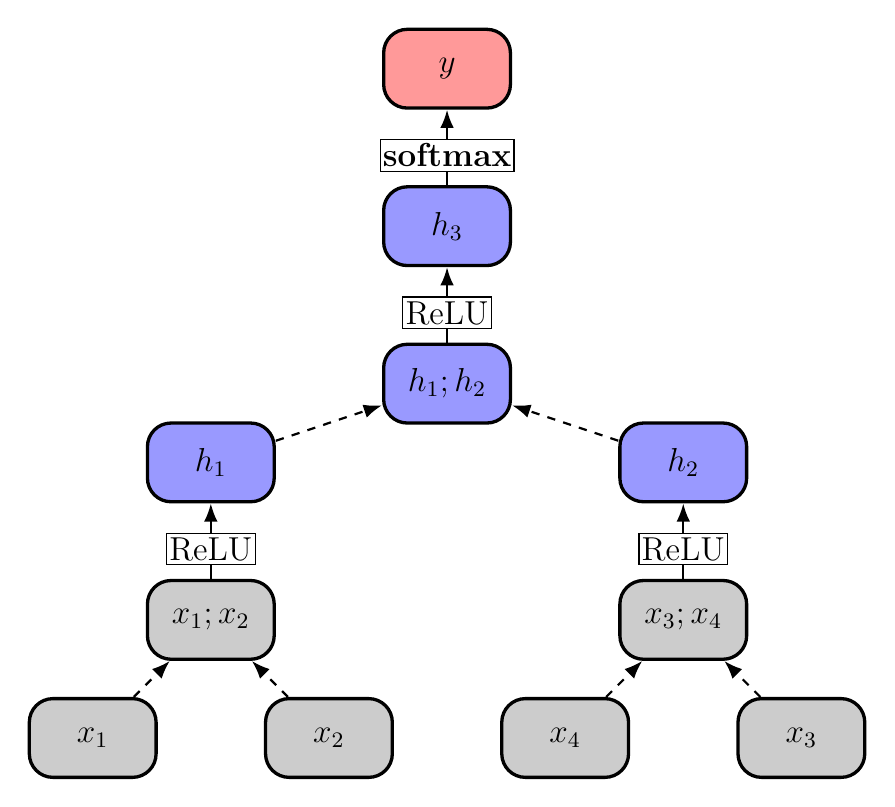
\begin{tikzpicture}[
      % GLOBAL CFG
      font=\sf \large,
      >=LaTeX,
      % Styles
      rep/.style={% For representations
        rectangle,
        rounded corners=3mm,
        draw,
        very thick,
        minimum height =1cm,
        minimum width=1.61cm
      },
      function/.style={%For functions
        ellipse,
        draw,
        inner sep=1pt
      },
      gt/.style={% For internal inputs
        rectangle,
        draw,
        minimum width=5mm,
        minimum height=4mm,
        inner sep=1pt
      },
      function/.style={
        rectangle,
        draw,
        minimum width=5mm,
        minimum height=4mm,
        inner sep=1pt
      },
      arrowconcat/.style={% Arrows for concatenation
        rounded corners=.25cm,
        dashed,
        thick,
        ->,
      },
      arrowfunction/.style={% Arrows for concatenation
        rounded corners=.25cm,
        thick,
        ->,
      }
      ]

      % Start drawing the thing...
      % Draw the cell:
      \node [rep, fill=\inputcolor] (input1) at (-4.5,1.5){$x_1$} ;
      \node [rep, fill=\inputcolor] (input2) at (-1.5,1.5){$x_2$} ;
      \node [rep, fill=\inputcolor] (concat) at (-3,3){$x_1;x_2$} ;
      \draw [arrowconcat] (input1) -- (concat);
      \draw [arrowconcat] (input2) -- (concat);


      \node [rep, fill=\hiddencolor] (hidden) at (-3,5){$h_1$} ;
      \node [gt, minimum width=1cm] (relu1) at (-3,4-0.1) {$\ReLU$};
      \draw [arrowfunction] (concat) -- (relu1) -- (hidden);


      \node [rep, fill=\inputcolor] (input3) at (4.5,1.5){$x_3$} ;
      \node [rep, fill=\inputcolor] (input4) at (1.5,1.5){$x_4$} ;
      \node [rep, fill=\inputcolor] (concat2) at (3,3){$x_3;x_4$} ;
      \draw [arrowconcat] (input3) -- (concat2);
      \draw [arrowconcat] (input4) -- (concat2);


      \node [rep, fill=\hiddencolor] (hidden2) at (3,5){$h_2$} ;
      \node [gt, minimum width=1cm] (relu2) at (3,4-0.1) {$\ReLU$};
      \draw [arrowfunction] (concat2) -- (relu2) -- (hidden2);


      \node [rep,fill=\hiddencolor] (hiddenconcat) at (0,6){$h_1;h_2$};
      \draw [arrowconcat] (hidden2) -- (hiddenconcat);
      \draw [arrowconcat] (hidden) -- (hiddenconcat);


      \node [rep, fill=\hiddencolor] (hidden3) at (0,8){$h_3$} ;
      \node [gt, minimum width=1cm] (relu3) at (0,7-0.1) {$\ReLU$};
      \draw [arrowfunction] (hiddenconcat) -- (relu3) -- (hidden3);


      \node [rep,fill=\outputcolor] (output) at (0,10){$y$} ;
      \node [gt, minimum width=1cm] (softmax) at (0,9-0.1) {$\softmax$};
      \draw [arrowfunction] (hidden3) -- (softmax) -- (output);

    \end{tikzpicture}
  }
  \caption{A single layer network pretrained on equality computing hierarchical equality.}
  \label{fig:models:premack}
\end{figure}


\section{Pretraining}\label{app:pretraining}

Our pretraining model closely resembles the models used for our main experiments. It defines a feed-forward network with a multitask objective. For an example $i$ and task $j$:
%
\begin{align}
  h_{i} &= \ReLU\left( E[i]W_{xh} + b_{h} \right) \\
  y_{i,j} &= \softmax(h^{i}W_{hy}^{j} + b_{y}^{j})
\end{align}
%
where $E[i]$ is the vector representation for example $i$ in the embedding matrix $E$. The overall objective of the model is to maximize the sum of the task objective functions. For $N$ examples, $J$ tasks, and $K_{j}$ the number of classes for task $j$:
%
\begin{equation}
  \max(\theta)
  \quad
  \frac{1}{N}
  \sum_{i=1}^{N}
  \sum_{j=1}^{J}
  \sum_{k=1}^{K_{j}}
  y^{i,j,k} \log \left( h_{\theta}(i)^{j,k} \right)
\end{equation}
%
where $y^{i,j,k}$ is the correct label for example $i$ in task $j$ and $p^{i,j,k}$ is the predicted value for example $i$ in task $j$.

For the experiments in the paper, we initialize $E$ randomly and then, for pretraining on $J$ tasks, we create a random binary vector of length $J$ for each row in $E$. Each dimension (task) in $J$ is independent of the others.

Our motivation for pretraining is to update the embedding $E$ so that its representations contain rich structure that can be used by subsequent models. To achieve this, we backpropagate errors through the network and into $E$.

In our experiments, we always pretrain for 10 iterations. This choice is motivated primarily by computational costs; additional pretraining iterations greatly increase experiment run-times, though they do have the potential to imbue the representations with even more useful structure.


\section{Model optimization details}\label{app:optimization}

The feed forward networks for basic and hierarchical equality were implemented using the multi-layer perception from sklearn and a cross entropy function was used to compute the prediction error. The recursive LSTM network for the sequential ABA task was implemented using PyTorch and a mean squared error function was used to compute the prediction error. The networks for pretraining representations and for the hierarchical equality task were also implemented using PyTorch, with cross-entropy loss functions used to compute the prediction errors. For all models, Adam optimizers \citep{Kingma:Ba:2015} were used. For all models, a hyperparameter search was run over learning rate values of \{0.00001, 0.0001, 0.001\} and l2 normalization values of \{0.0001, 0.001, 0.01\} for each hidden dimension and input dimension mentioned in the paper.


\section{Localist and binary feature representations prevent generalization}\label{app:generalization}

The method of representation impacts whether there is a natural notion of similarity between entities and the ability of models to generalize to examples unseen in training. These two attributes are deeply related; if there is a natural notion of similarity between vector representations, then models can generalize to inputs with representations that are similar to those seen in training.

In order to discuss how representation impacts generalization, we will need explain some properties of how neural models are trained. Standard neural models, including all models in the paper, begin with applying a linear layer to the input vector where no two input units are connected to the same weight. An easily observed fact about the back-propagation learning algorithm is that, if a unit of the input vector is always zero during training, then any weights connected to that unit and only that unit will not change from their initialized values during training. This means that, when a standard neural model is evaluated on an input vector that has a non-zero value for a unit that was zero throughout training, untrained weights are used and behavior is unpredictable.

Localist representations are orthogonal and equidistant from one another so there is no notion of similarity and consequently standard neural models have no ability to generalize to new examples. No two representations share a non-zero unit, and so when models are presented with inputs unseen in training, untrained weights are used and the resulting behavior is again unpredictable.

Distributed representations with binary features also limit generalization, though less severely than localist representations. Localist representations prevent generalization to entities unseen during training, while binary feature representations prevent generalization to features unseen during training. For example, if color and shape are represented as binary features, and a red square and blue circle are seen in training, then a model could generalize to the unseen entities of a blue circle or a red square. However, if no entity that is a circle is seen during training, then the binary feature representing the property of being a circle is zero throughout training and untrained weights are used when the model is presented with a entity that is a circle during testing, which results in unpredictable behavior.

Distributed representations with analog features do not inhibit generalization in the same way. If height is represented as a binary feature, then a single unit represents all height values and is always non-zero. Non-featural representations similarly do not inhibit generalization, because all units for all representations are non-zero and the network can learn parameters that create complex associations between these entities and its task labels.


\section{An analytic solution to identity with a feed forward network}\label{app:equality-solution}

We now show that our feed forward networks can solve the same--different problem we pose, in the following sense: for any set of inputs, we can find parameters $\theta$ that perfectly classify those inputs. At the same time, we also show that there are always additional inputs for which $\theta$ makes incorrect predictions.

Here are the parameters of a feed forward neural network that performs a binary classification task
%
\[ \texttt{ReLu}(\begin{pmatrix} x_1 \\ x_2  \end{pmatrix}^T \begin{pmatrix} W^{11} & W^{12}\\ W^{21}& W^{22} \end{pmatrix}) \begin{pmatrix} v^{11} & v^{12} \\ v^{21} & v^{22} \end{pmatrix} + \begin{pmatrix}b_1 &b_2 \end{pmatrix}= \begin{pmatrix} o_1 & o_2\end{pmatrix}\]
%
where, if $n$ is the dimension of entity embeddings used, then
%
\begin{align*}
  x, y,v^{11}, v^{12}, v^{21}, v^{22} &\in \mathbb{R}^{n \times 1} \\
  W^{11}, W^{12},W^{21}, W^{22} &\in \mathbb{R}^{n \times n} \\
  b_1, b_2, o_1, o_2 &\in \mathbb{R}
\end{align*}
%
Given an input $(x_1,x_2)$, if the output $o_1$ is larger than $o_2$, then one class is predicted; if the output $o_2$ is larger that $o_1$, then the other class is predicted. When the two outputs are equal, the network has predicted that both classes are equally likely and we can arbitrarily decide which class is predicted. In this case, the output $o_1$ predicts the two inputs, $x_1$ and $x_2$, are in the identity relation and the output $o_2$ predicts the two inputs are not. Now we specify parameters to provide an analytic solution to the identity relation using this network
%
\[ \texttt{ReLu}(\begin{pmatrix} x_1 \\ x_2 \end{pmatrix}^T \begin{pmatrix} I & -I\\ -I& I \end{pmatrix}) \begin{pmatrix} \vec{1} & \vec{0} \\ \vec{1} & \vec{0} \end{pmatrix} + \begin{pmatrix}b_1 &b_2 \end{pmatrix}= \begin{pmatrix} o_1 & o_2\end{pmatrix}\]
%
where $I$ is the identity matrix, $-I$ is the negative identity matrix, and $\vec{1}$ and $\vec{0}$ are the two vectors in $\mathbb{R}^n$ that have all zeros and all ones, respectively. The output values, given an input, are
%
\[ o_1 = \sum_{i = 1}^{n}|(x_1)_i- (x_2)_i|+ b_1 \qquad \quad  o_2 = b_2\]
%
where two parameters are left unspecified, $b_1, b_2$. We present a visualization in Figure~\ref{fig:analyticff} of how the analytic solution to identity of this network changes depending on the values of two bias terms. In this example, the network receives two one-dimensional inputs, $x_1$ and $x_2$. If the ordered pair of inputs is in the shaded area on the graph, then they are predicted to be in the identity relation. If in the unshaded area, they are predicted not to be. The dotted line is where the network predicts the two classes to be equally likely.


\begin{figure}[h]
  \centering
  \newcommand\X{2}
  \newcommand\E{0.03}
  % \tcbox{
  \begin{tikzpicture}[scale=0.7]
    \centering
    \filldraw[fill=black, opacity=0.1]
    (-5,-5 + \X)--(5-\X,5) -- (5,5) -- (5,5 - \X)--(-5+ \X,-5)--(-5,-5)--(-5,-5 + \X);
    \draw[<->,ultra thick] (-5,0)--(5,0) node[right]{$x_1$};
    \draw[<->,ultra thick] (0,-5)--(0,5) node[above]{$x_2$};
    \draw[<->,thick] (-5,-5)--(5,5) ;
    \draw[<->,thick, dashed] (-5,-5 + \X)--(5-\X,5) ;
    \draw[<->,thick,dashed] (-5+ \X,-5)--(5,5 - \X) ;
    \draw [decorate,decoration={brace,amplitude=12pt},xshift=-0pt,yshift=0pt]
    (3 - \X/2 + \E ,3 + \X/2- \E) -- (3-\E,3+\E) node [black,midway, xshift=12pt,yshift=12pt]
    { \rotatebox{-45}{$\scriptstyle b_1 - b_2$}};
  \end{tikzpicture}
  % }
  \caption{A visual representation of how the analytic solution to identity of a single layer feed forward network changes depending on the values of two bias terms, $b_1,b_2$.}
  \label{fig:analyticff}
\end{figure}

The network predicts $x_1$ and $x_2$ to be in the identity relation if $\sum_{i = 1}^{n}|x_i- y_i| < b_1-b_2$ which is visualized as the points between two parallel lines above and below the solution line $x_1 = x_2$. As the difference $b_1-b_2$ gets smaller and smaller, the two lines that bound the network's predictions get closer and closer to the solution line. However, as long as $b_1-b_2$ is positive, there will always be inputs of the form $(r,r+(b_1-b_2)/2)$ that are false positives. For any set of inputs, we can find bias values that result in the network correctly classifying those inputs, but for any bias values, we can find an input that is incorrectly classified by those values. In other words, we have an arbitrarily good solution that is never perfect. We provide a proof below that there is no perfect solution and so this is the best outcome possible. However, if we were to decide that, if the network predicts that an input is equally likely in either class, then this input is predicted to be in the identity relation, we could have a perfect solution with $b_1= b_2$.

Here is proof that a perfect solution is not possible. A basic fact from topology is that the set $\{x: f(x) < g(x)\}$ is an open set if $f$ and $g$ are continuous functions. Let $N_{o_1}$ and $N_{o_2}$ be the functions that map an input $(x_1,x_2)$ to the output values of the neural network, $o_1$ and $o_2$, respectively. These functions are continuous. Consequently, the set $C = \{(x_1,x_2): N_{o_2}(x_1,x_2) < N_{o_1}(x_1,x_2)\}$, which is the set of inputs that are predicted to be in the equality relation, is open.

With this fact, we can show that, if the neural network correctly classifies any point on the solution line $x_1 = x_2$, then it must incorrectly classify some point not on the solution line. Suppose that $C$ contains some point $(x,x)$. Then, by the definition of an open set, $C$ contains some $\epsilon$ ball around $(x,x)$, and therefore $C$ contains $(x,x+\epsilon)$, which is not on the solution line $x_1=x_2$. Thus, $C$ can never be equal to the set $\{(x_1,x_2):x_1=x_2\}$. So, because $C$ is the set of inputs classified as being in the equality relation by the neural network, a perfect solution cannot be achieved. Thus, we can conclude our arbitrarily good solution is the best we can do.


\section{An analytic solution to ABA sequences}\label{sec:analyticlm}


Here are the parameters of a long short term memory recursive neural network (LSTM):
%
\begin{align*}
  f_t &= \sigma(x_t W_f  + h_{t-1} U_f  + b_f) \\
  i_t &= \sigma(x_t W_i  + h_{t-1} U_i + b_i) \\
  o_t &= \sigma(x_t W_o +  h_{t-1} U_o + b_o)\\
  c_t &= f_t \circ c_{t-1} + i_t \circ \ReLU(x_tW_c + h_{t-1}U_c + b_c) \\
  h_t &= o_t \circ \ReLU(c_t) \\
  y_t &= h_tV
\end{align*}
%
where, if $n$ is the representation size and $d$ is the network hidden dimension, then
%
\begin{align*}
  x_t \in \mathbb{R}^n, f_t, i_t, o_t,  h_t, c_t &\in \mathbb{R}^d\\
  W \in \mathbb{R}^{n \times d}, U &\in \mathbb{R}^{d \times d}\\
  V \in \mathbb{R}^{d \times n}, b &\in \mathbb{R}^d
\end{align*}
%
and $\sigma$ is the sigmoid function. The initial hidden state $h_0$ and initial cell state $c_0$ are both set to be the zero vector. We say that an LSTM model with specified parameters has learned to produce ABA sequences if the following holds: when the network is seeded with some entity vector representation as its first input, $x_1$, then the output $y_1$ is not equal to $x_1$ and at the next time step the output $y_2$ is equal to $x_1$.

We let $d = 2n + 1$ and assign the following parameters, which provide an analytic solution to producing ABA sequences:
%
\begin{align*}
  f_t &= \sigma(x_t \textbf{0}_{n\times d} + h_{t-1}\textbf{0}_{d \times d} + \textbf{N}_{d}) \\
  i_t &= \sigma(x_t\textbf{0}_{n\times d} + h_{t-1}\begin{bmatrix} -4 \dots -4 \\ \textbf{0}_{2n\times n} \end{bmatrix}  + \textbf{N}_d)   \\
  o_t &= \sigma(x_t\textbf{0}_{n\times d} +  h_{t-1} \begin{bmatrix} 1 \dots 1 \\ \textbf{0}_{2n\times n} \end{bmatrix} + \textbf{0}_{d})\\
  c_t &= f_t \circ c_{t-1} + \\
  & i_t \circ \ReLU\left(x_t \begin{bmatrix} 0 &  & \\ \vdots & -I_{n \times n} & I_{n \times n}\\ 0 & &  \end{bmatrix} + h_{t-1}\textbf{0}_{d \times d} + \begin{bmatrix} N & 0 \dots 0\end{bmatrix}\right) \\
  h_t &= o_t \circ \ReLU(c_t)\\
  y &= h_t \begin{bmatrix} 0 \dots 0 \\ -I_{n \times n} \\ I_{n \times n}  \end{bmatrix}
\end{align*}
%
Where $\textbf{0}_{j\times k}$ is the $j \times k$ zero matrix, $\textbf{m}_k$ is a $k$ dimensional vector with each element having the value $m$, $I_{n\times n}$ is the $n \times n$ identity matrix, and $N$ is some very large number.  Now we show that these parameters achieve an increasingly good solution as $N$ increases. When a value involves the number $N$, we will simplify the computation by saying what that value is equal to as $N$ approaches infinity. We begin with an arbitrary input $x_1$ and the input and hidden state intialized to zero vectors:
%
\[
  h_0 = \textbf{0}_d \qquad c_0 = \textbf{0}_d
\]
%
The gates at the first time step are easy to compute, as the cell state and hidden state are zero vectors so the gates are equal to the sigmoid function applied to their respective bias vectors. The forget gate is completely open, the output gate is partially open, and the input gate is fully open:
%
\begin{align*}
  f_1 &= \sigma(\textbf{N}_d) \approx \textbf{1}_d \\
  o_1 &= \sigma(\textbf{0}_d) = \textbf{0.5}_d \\
  i_1 &=  \sigma(\textbf{N}_d) \approx \textbf{1}_d
\end{align*}
%
Then we compute the cell and hidden states at the first timestep. The cell state encodes the information of the input vector, so it can be used to recover the vector at a later time step and receives no information from the previous cell state despite the forget gate being open, because the previous cell state is a zero vector. The hidden state is the cell state scaled by one half.
%
\begin{align*}
  c_1 &= \textbf{N}_d\circ \textbf{0}_d+ \\
      & \textbf{1}_d \circ \ReLU\left(x_1\begin{bmatrix} 0 &  & \\ \vdots & -I_{n \times n} & I_{n \times n}\\ 0 & &  \end{bmatrix} + \begin{bmatrix} N & 0 \dots 0\end{bmatrix}\right) \\
      & = \ReLU\left( \begin{bmatrix} N & -x_1 & x_1 \end{bmatrix}\right) \\[1ex]
  h_1 &= \textbf{0.5}_d\ReLU \left(\ReLU( \begin{bmatrix} N & -x_1 & x_1 \end{bmatrix})\right) \\
      &= \textbf{0.5}_d\circ \ReLU( \begin{bmatrix} N & -x_1 & x_1 \end{bmatrix})
\end{align*}
%
At the next time step, the forget gate remains fully open, the open gate changes from partially open to fully open, and the input gate changes from fully open to fully closed:
%
\begin{align*}
  f_2 &= \textbf{N}_d \\[2ex]
  o_2 &= \sigma(y_1\textbf{0}_{n\times d} + h_{1}\begin{bmatrix} 1 \dots 1 \\ \textbf{0}_{2n\times n} \end{bmatrix}  + \textbf{0}_d) \\
  &= \sigma(\textbf{0.5}_d\circ \ReLU\left( \begin{bmatrix} N & -x_1 & x_1 \end{bmatrix}\right)\begin{bmatrix} 1 \dots 1 \\ \textbf{0}_{2n\times n} \end{bmatrix}  + \textbf{0}_d)  \\
  &=  \sigma(\textbf{0.5}_d\circ \textbf{N}_d) \approx \textbf{1}_d \\[2ex]
  i_2 &= \sigma(y_1\textbf{0}_{n\times d} + h_{1}\begin{bmatrix} -4 \dots -4 \\ \textbf{0}_{2n\times n} \end{bmatrix}  + \textbf{N}_d)  \\
  &= \sigma(\textbf{0.5}_d\circ \ReLU\left( \begin{bmatrix} N & -x_1 & x_1 \end{bmatrix}\right)\begin{bmatrix} -4 \dots -4 \\ \textbf{0}_{2n\times n} \end{bmatrix}  + \textbf{N}_d)   \\
  &=  \sigma(\textbf{0.5}_d\circ\textbf{-4N}_d + \textbf{N}_d) \approx \textbf{0}_d
\end{align*}
%
Then we compute the cell and hidden states for the second timestep. Because the forget gate is completely open and the input gate is completely closed, the cell state remains the same. Because the output gate is completely open, the hidden state is the same as the cell state.
%
\begin{align*}
  c_2 &= \textbf{1}_d \circ \ReLU \left( \begin{bmatrix} N & -x_1 & x_1 \end{bmatrix}\right) +\\
      & \textbf{0}_d\circ \ReLU(x_2\begin{bmatrix} 0 &  & \\ \vdots & -I_{n \times n} & I_{n \times n}\\ 0 & &  \end{bmatrix} + \begin{bmatrix} N & 0 \dots 0\end{bmatrix}) \\
      &= \ReLU \left( \begin{bmatrix} N & -x_1 & x_1 \end{bmatrix}\right) \\[2ex]
  h_2 &= \textbf{1}_d \circ \ReLU\left(\ReLU ( \begin{bmatrix} N & -x_1 & x_1 \end{bmatrix})\right) \\
      &= \ReLU \left( \begin{bmatrix} N & -x_1 & x_1 \end{bmatrix}\right)
\end{align*}
%
With the hidden states for the first and second time steps, we can compute the output values and find that the output at the first time step is the initial input vector scaled by one half and the output at the second time step is the initial input vector.

\begin{align*}
  y_1 &= h_1\begin{bmatrix} 0 \dots 0 \\ -I_{n \times n} \\ I_{n \times n}  \end{bmatrix} = \textbf{0.5}_d\circ \ReLU\left( \begin{bmatrix} N & -x_1 & x_1 \end{bmatrix}\right) \begin{bmatrix} 0 \dots 0 \\ -I_{n \times n} \\ I_{n \times n}  \end{bmatrix} \\
      &= \textbf{0.5}_d\circ x_1\\
  y_2 &= h_2\begin{bmatrix} 0 \dots 0 \\ -I_{n \times n} \\ I_{n \times n}  \end{bmatrix} = \texttt{ReLu} ( \begin{bmatrix} N & -x_1 & x_1 \end{bmatrix}) \begin{bmatrix} 0 \dots 0 \\ -I_{n \times n} \\ I_{n \times n}  \end{bmatrix} = x_1
\end{align*}
%
Then, because $y_1 = \textbf{0.5}_d\circ x_1 \not = x_1$ and $y_2 = x_1$, this network produces ABA sequences.


\newpage


\section{Additional results plots}


\subsection{Model 1 for basic same--different}\label{app:model1-results}

\Figref{fig:model1} explores a wider range of hidden dimensionalities for Model~1 applied to the basic same--differerent task. As in the paper, the lines correspond to different embedding dimensionalities. \Figref{fig:model1-rep} is repeated from \figref{fig:equality--smallresults}.

\begin{figure}[H]
  \centering

  \begin{subfigure}{0.45\linewidth}
    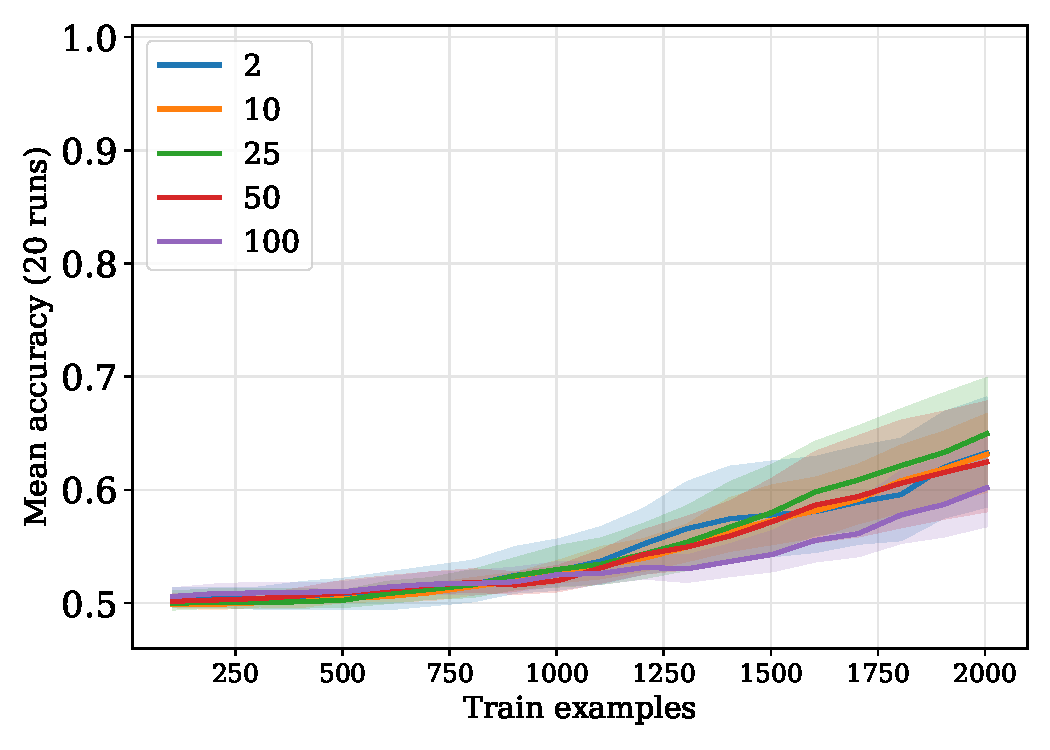
\includegraphics[width=1\textwidth]{../fig/equality-train_size-embed_dim-hidden_dim=2.pdf}
    \caption{Hidden dimensionality 2.}
  \end{subfigure}
  \hfill
  \begin{subfigure}{0.45\linewidth}
    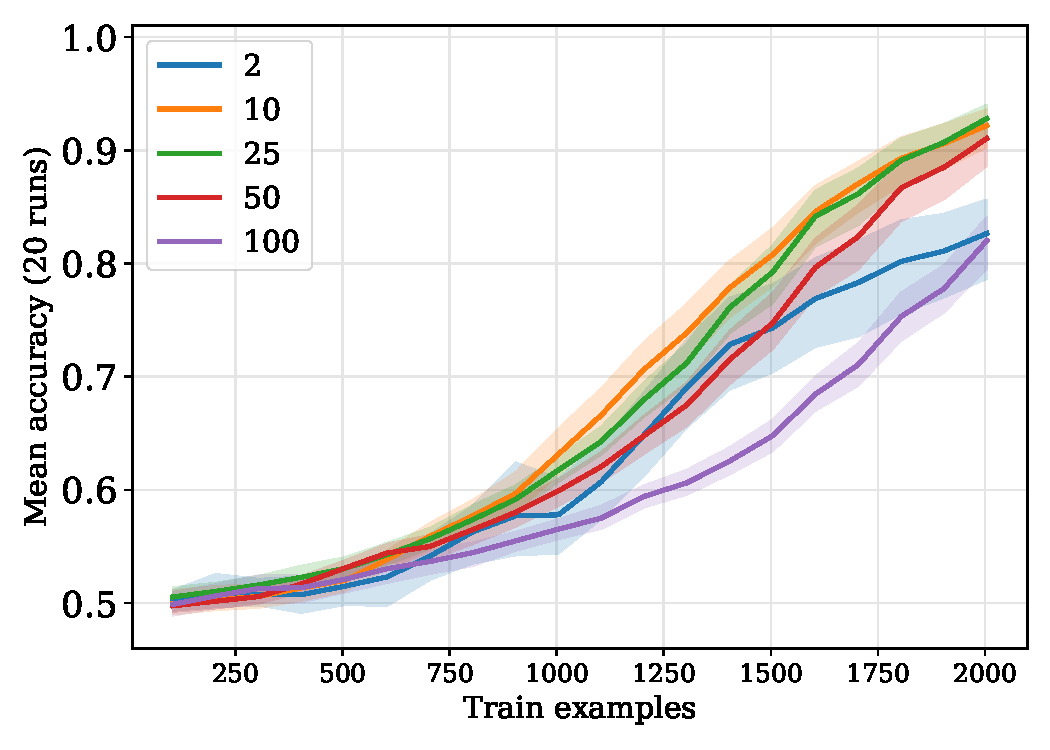
\includegraphics[width=1\textwidth]{../fig/equality-train_size-embed_dim-hidden_dim=10.pdf}
    \caption{Hidden dimensionality 10.}
  \end{subfigure}

  \vspace{24pt}

  \begin{subfigure}{0.45\linewidth}
    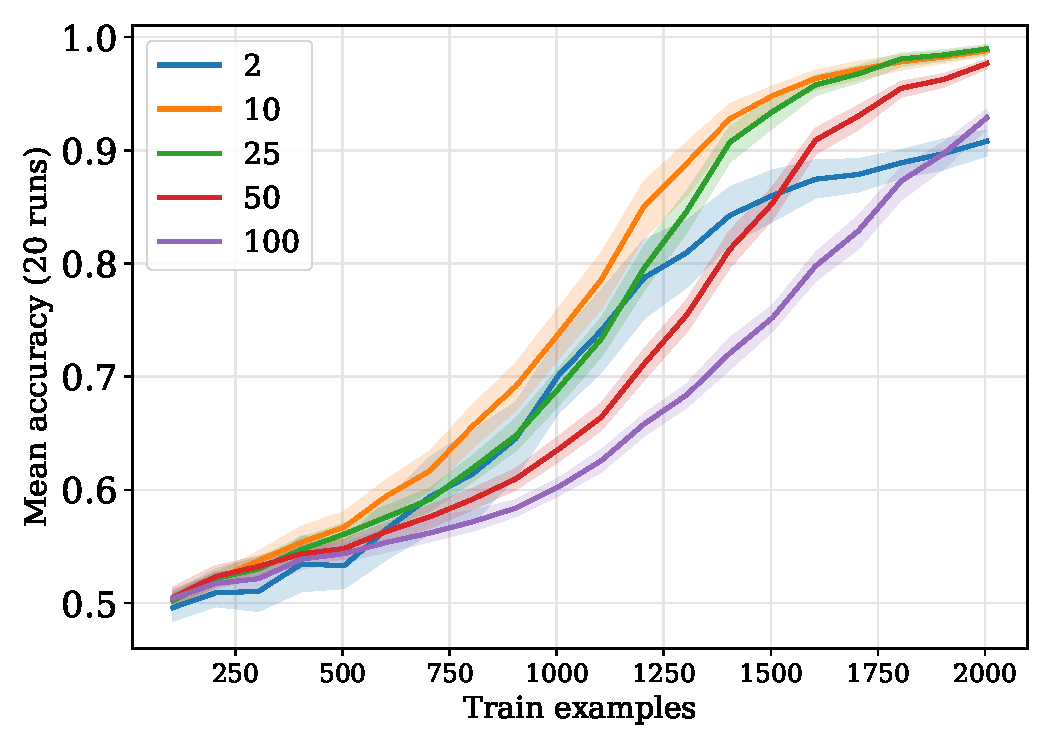
\includegraphics[width=1\textwidth]{../fig/equality-train_size-embed_dim-hidden_dim=25.pdf}
    \caption{Hidden dimensionality 25.}
  \end{subfigure}
  \hfill
  \begin{subfigure}{0.45\linewidth}
    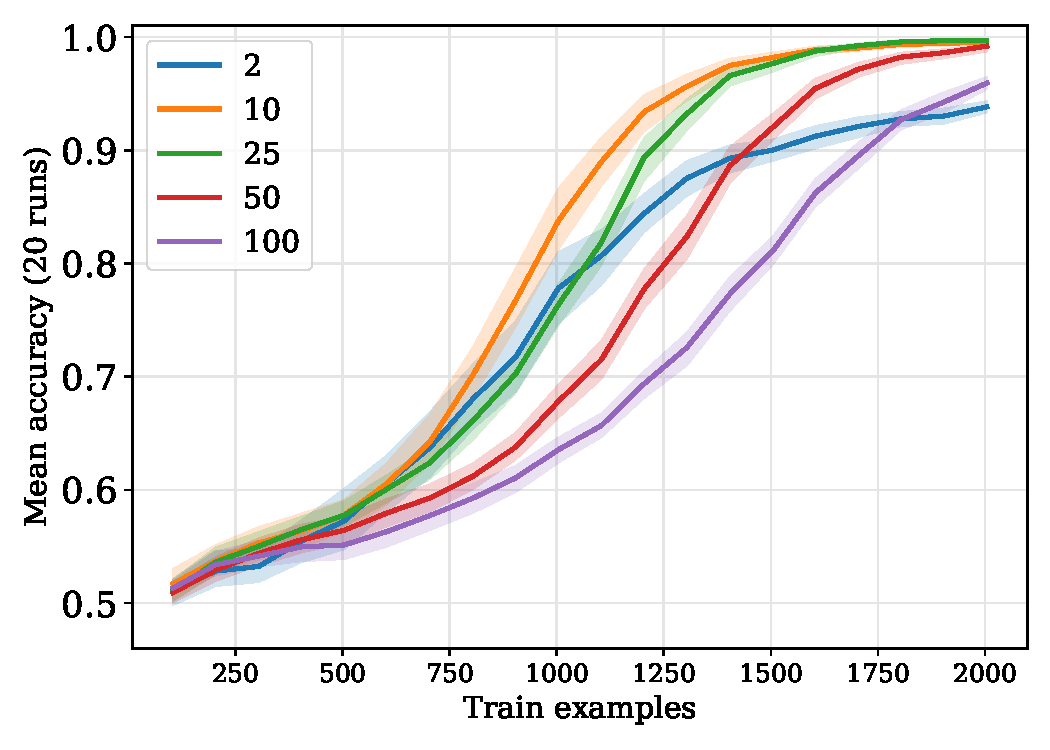
\includegraphics[width=1\textwidth]{../fig/equality-train_size-embed_dim-hidden_dim=50.pdf}
    \caption{Hidden dimensionality 50.}
  \end{subfigure}

  \vspace{24pt}

  \begin{subfigure}{0.45\linewidth}
    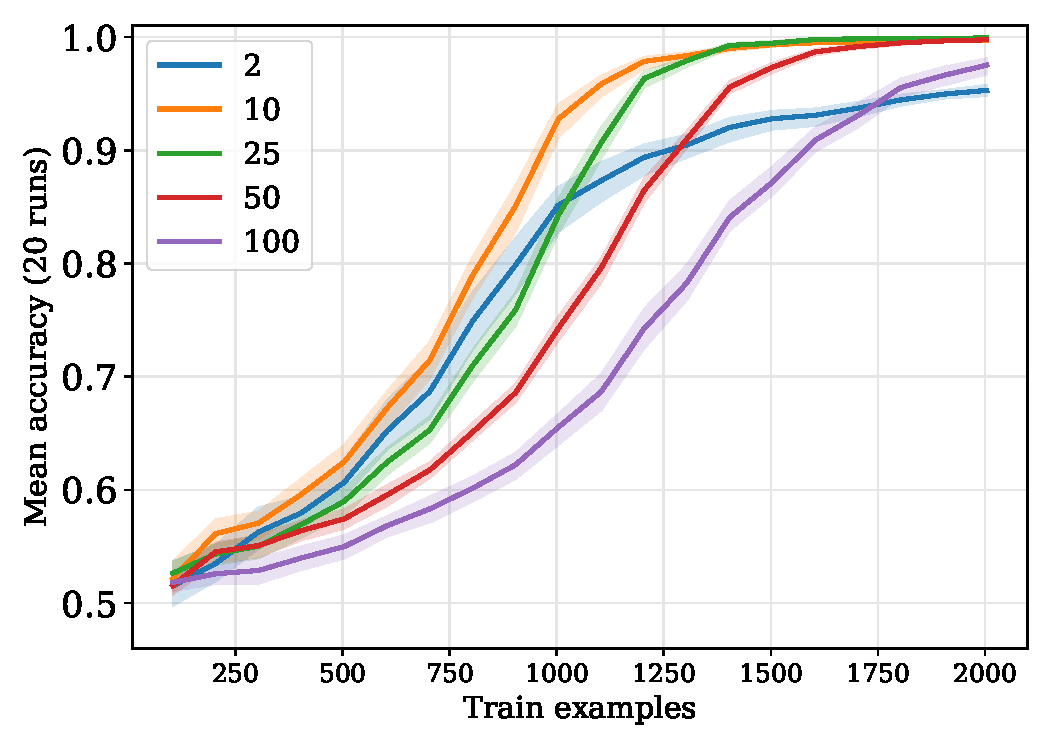
\includegraphics[width=1\textwidth]{../fig/equality-train_size-embed_dim-hidden_dim=100.pdf}
    \caption{Hidden dimensionality 100.}
    \label{fig:model1-rep}
  \end{subfigure}
  \caption{Results for Model 1 for basic same--different.}
  \label{fig:model1}
\end{figure}


\newpage


\subsection{Model 2 for sequential same--different}

\Figref{fig:model2} explores a wider range of hidden dimensionalities for Model~2 applied to the sequential ABA task. As in the paper, the lines correspond to different embedding dimensionalities. The full training set is presented to the model in multiple epochs. \Figref{fig:model2-rep} is repeated from \figref{fig:fuzzy-lm-pretrain-results}.

\begin{figure}[H]
  \centering

  \begin{subfigure}{0.45\linewidth}
    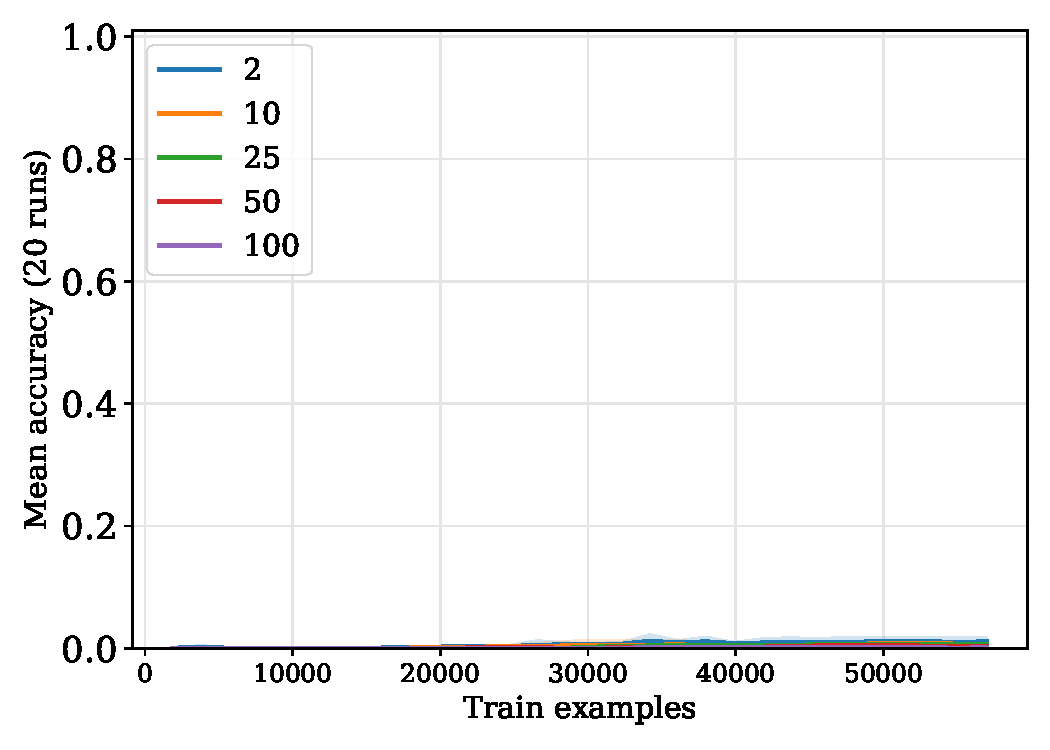
\includegraphics[width=1\textwidth]{../fig/fuzzy-lm-vocab20-pretrain-3tasks-train_size-embed_dim-hidden_dim=2.pdf}
    \caption{Hidden dimensionality 2.}
  \end{subfigure}
  \hfill
  \begin{subfigure}{0.45\linewidth}
    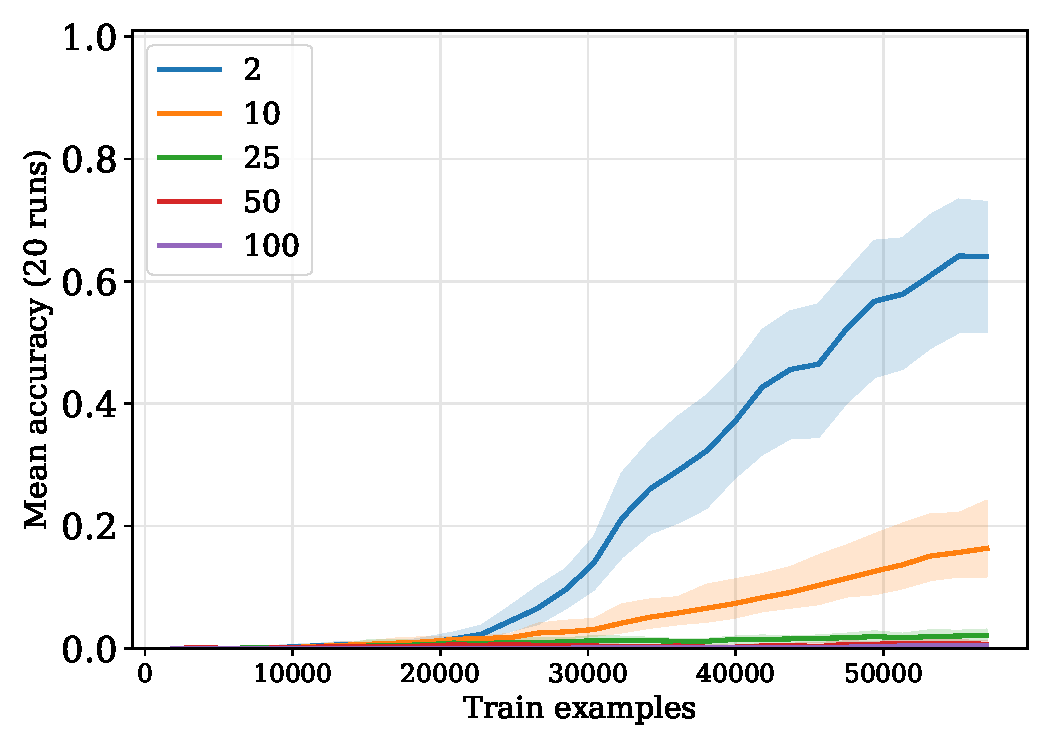
\includegraphics[width=1\textwidth]{../fig/fuzzy-lm-vocab20-pretrain-3tasks-train_size-embed_dim-hidden_dim=10.pdf}
    \caption{Hidden dimensionality 10.}
  \end{subfigure}

  \vspace{24pt}

  \begin{subfigure}{0.45\linewidth}
    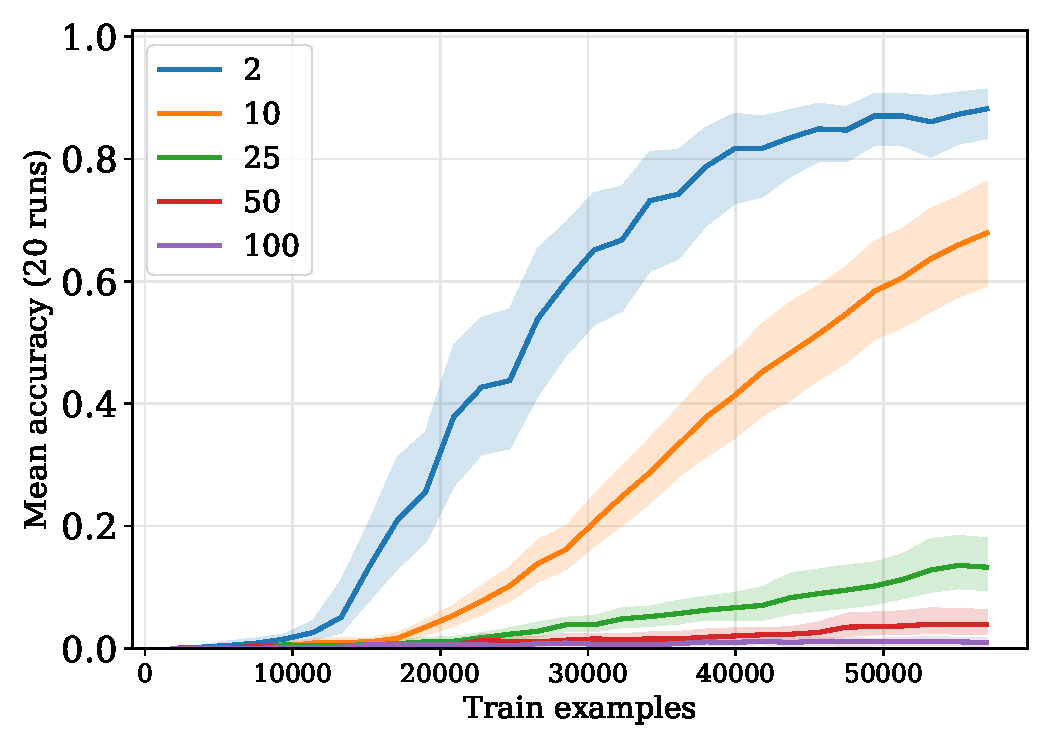
\includegraphics[width=1\textwidth]{../fig/fuzzy-lm-vocab20-pretrain-3tasks-train_size-embed_dim-hidden_dim=25.pdf}
    \caption{Hidden dimensionality 25.}
  \end{subfigure}
  \hfill
  \begin{subfigure}{0.45\linewidth}
    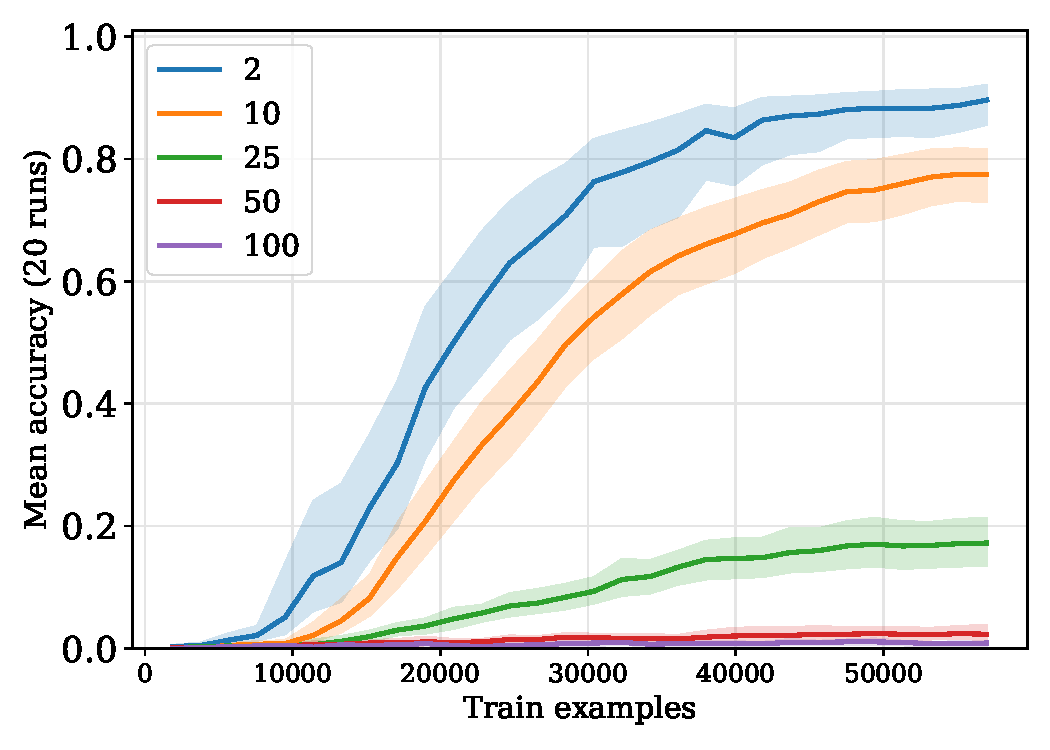
\includegraphics[width=1\textwidth]{../fig/fuzzy-lm-vocab20-pretrain-3tasks-train_size-embed_dim-hidden_dim=50.pdf}
    \caption{Hidden dimensionality 50.}
  \end{subfigure}

  \vspace{24pt}

  \begin{subfigure}{0.45\linewidth}
    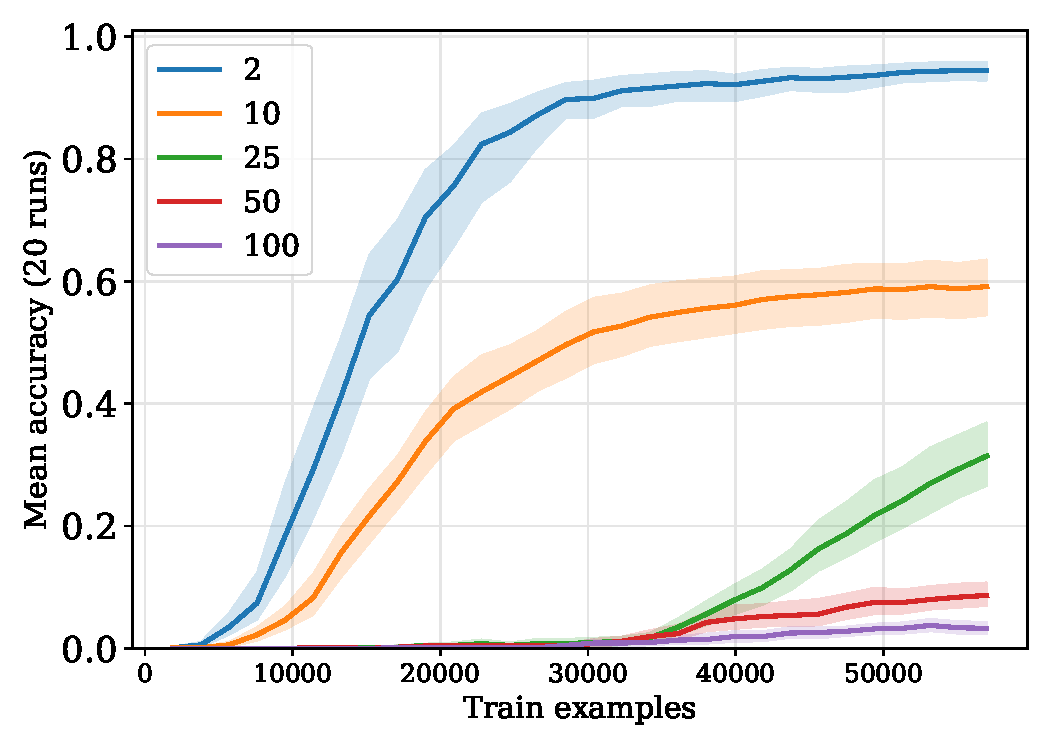
\includegraphics[width=1\textwidth]{../fig/fuzzy-lm-vocab20-pretrain-3tasks-train_size-embed_dim-hidden_dim=100.pdf}
    \caption{Hidden dimensionality 100.}
    \label{fig:model2-rep}
  \end{subfigure}

  \caption{Results for Model 2 for basic same--different, with a vocabulary size of 20.}
  \label{fig:model2}
\end{figure}


\newpage


\subsection{Model 1 for hierarchical same--different}\label{app:model1-premack}

\Figref{fig:model1:premack} shows the results of applying the model in \dasheg{eq:x2h-supp}{eq:h2y-supp} to the hierarchical same--different task. The only change from that model is that the inputs have dimensionality $4m$, since the four distinct representations in task inputs are simply concatenated.


\begin{figure}[H]
  \centering

  \begin{subfigure}{0.45\linewidth}
    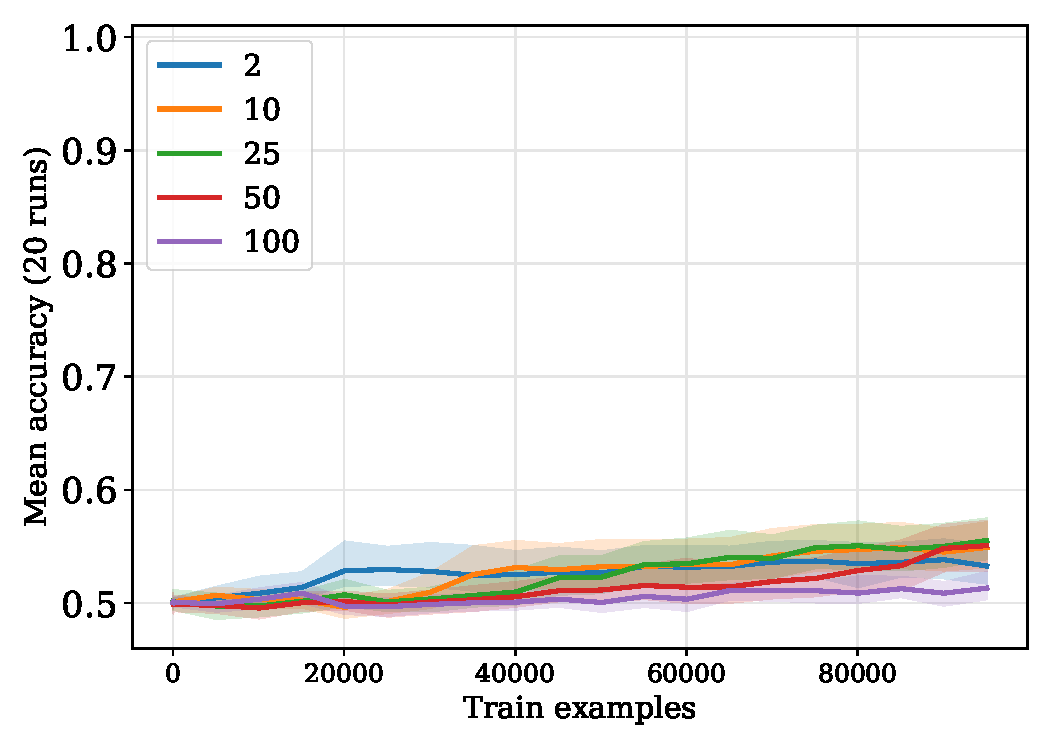
\includegraphics[width=1\textwidth]{../fig/flatpremack-h1-train_size-embed_dim-hidden_dim=2.pdf}
    \caption{Hidden dimensionality 2.}
  \end{subfigure}
  \hfill
  \begin{subfigure}{0.45\linewidth}
    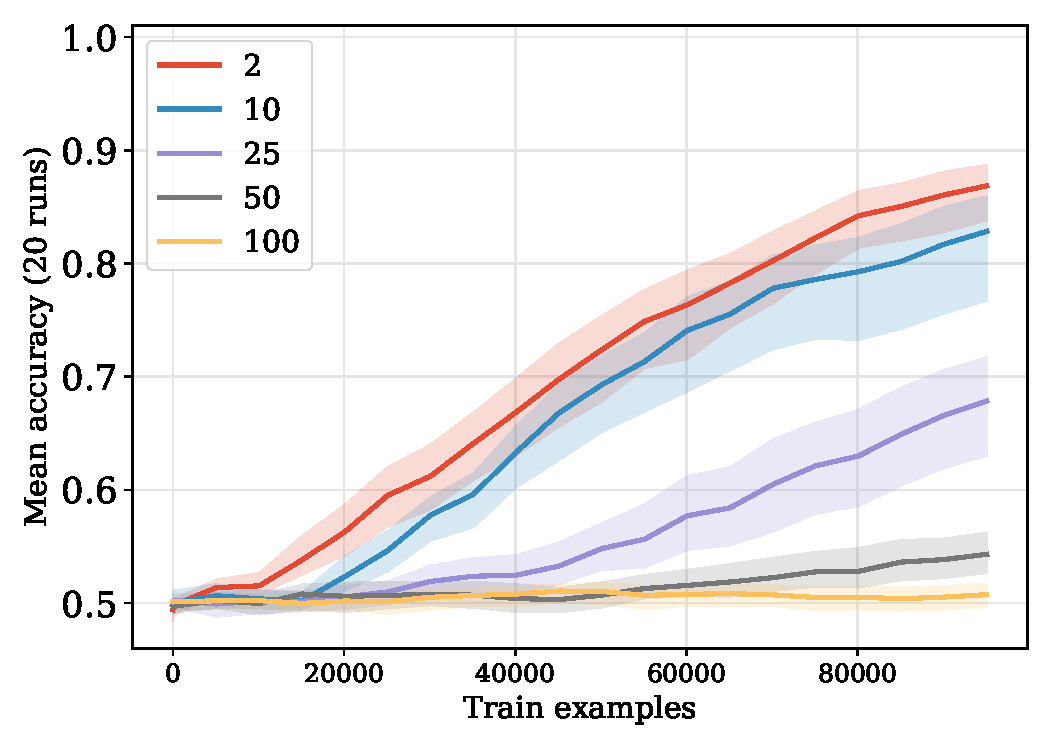
\includegraphics[width=1\textwidth]{../fig/flatpremack-h1-train_size-embed_dim-hidden_dim=10.pdf}
    \caption{Hidden dimensionality 10.}
  \end{subfigure}

  \vspace{24pt}

  \begin{subfigure}{0.45\linewidth}
    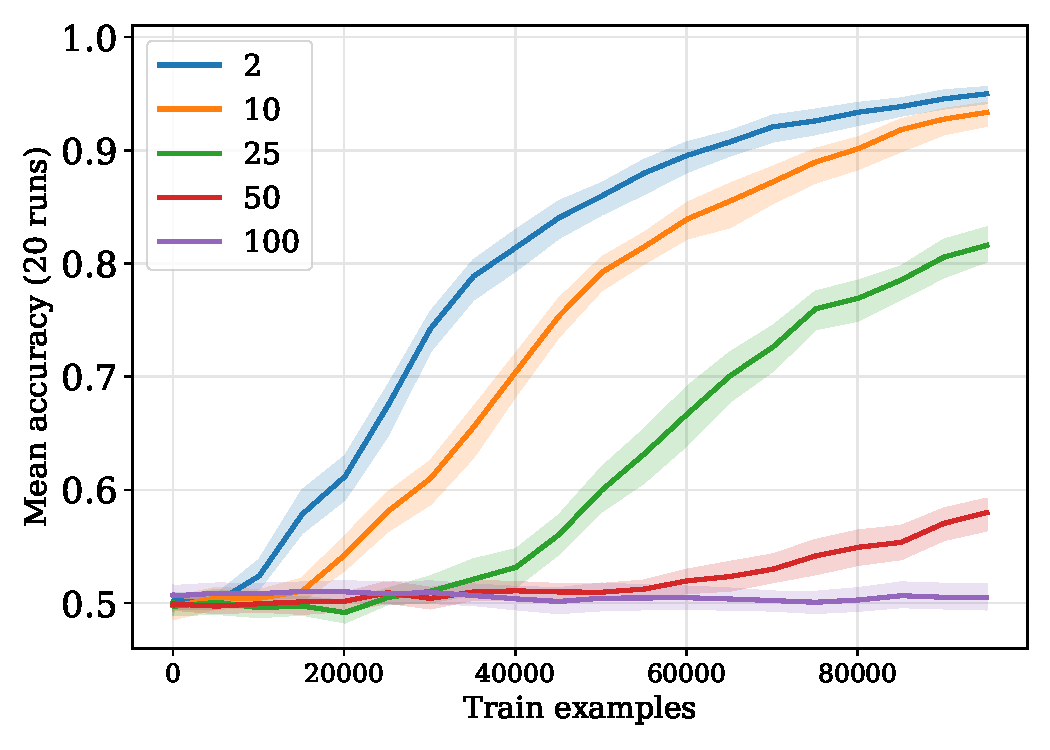
\includegraphics[width=1\textwidth]{../fig/flatpremack-h1-train_size-embed_dim-hidden_dim=25.pdf}
    \caption{Hidden dimensionality 25.}
  \end{subfigure}
  \hfill
  \begin{subfigure}{0.45\linewidth}
    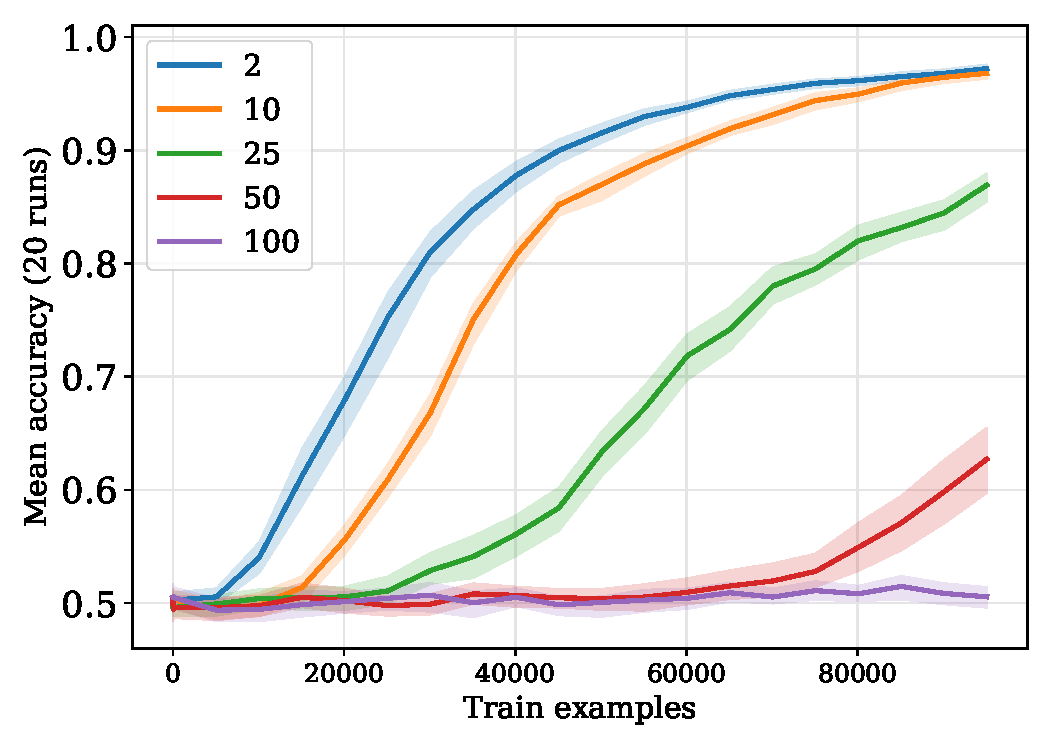
\includegraphics[width=1\textwidth]{../fig/flatpremack-h1-train_size-embed_dim-hidden_dim=50.pdf}
    \caption{Hidden dimensionality 50.}
  \end{subfigure}

  \vspace{24pt}

  \begin{subfigure}{0.45\linewidth}
    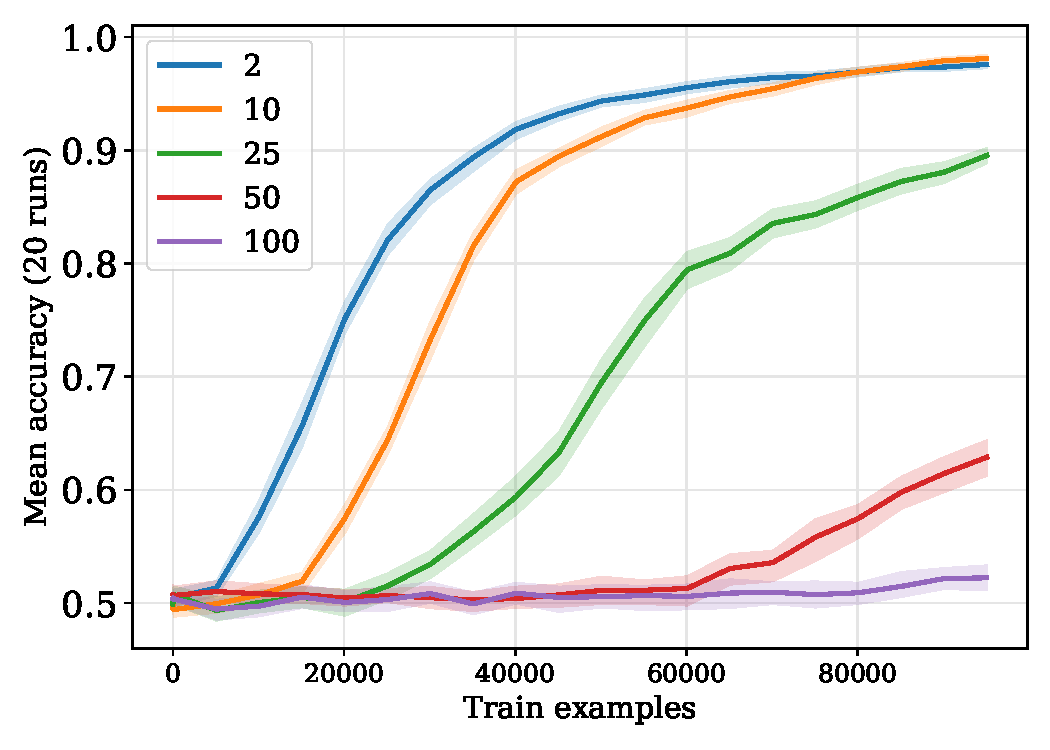
\includegraphics[width=1\textwidth]{../fig/flatpremack-h1-train_size-embed_dim-hidden_dim=100.pdf}
    \caption{Hidden dimensionality 100.}
  \end{subfigure}
  \caption{Results for Model 1 applied to the hierarchical same--different task.}
  \label{fig:model1:premack}
\end{figure}


\newpage


\subsection{Model 3a for hierarchical same--different}

\Figref{fig:model3a} shows the results of applying the model in \dasheg{eq:x2h1-supp}{eq:h2y2-supp} to the hierarchical same--different task. \Figref{fig:model3a-rep} is repeated from \figref{fig:premack-h2-flat-results}.

\begin{figure}[H]
  \centering

  \begin{subfigure}{0.45\linewidth}
    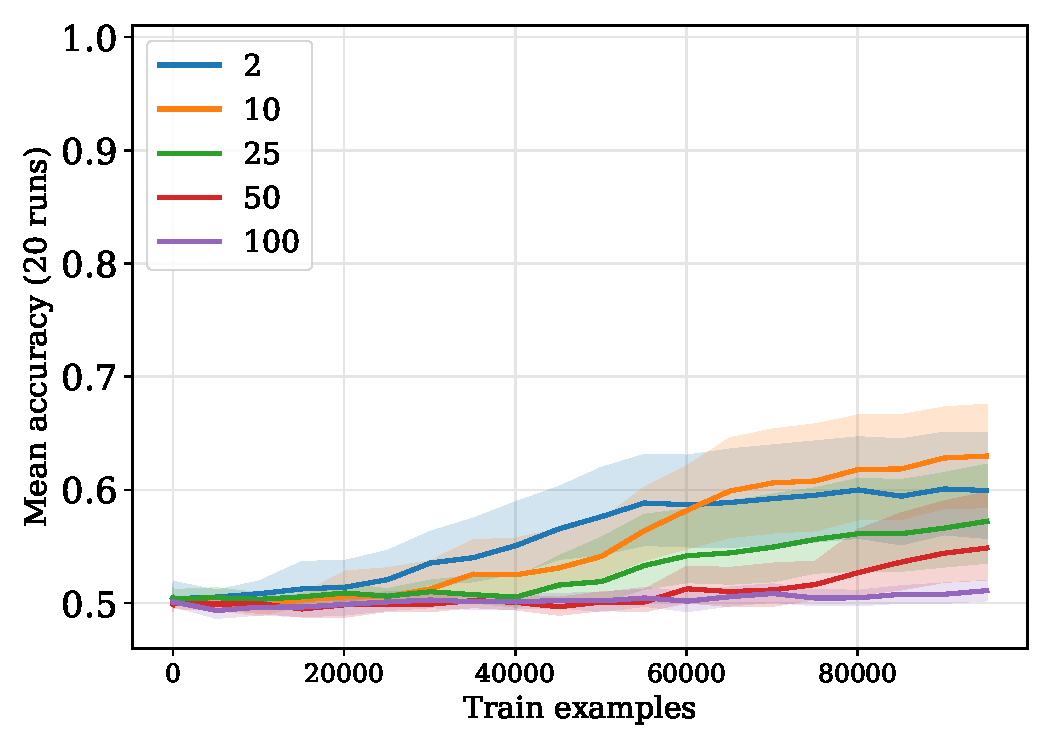
\includegraphics[width=1\textwidth]{../fig/flatpremack-h2-train_size-embed_dim-hidden_dim=2.pdf}
    \caption{Hidden dimensionality 2.}
  \end{subfigure}
  \hfill
  \begin{subfigure}{0.45\linewidth}
    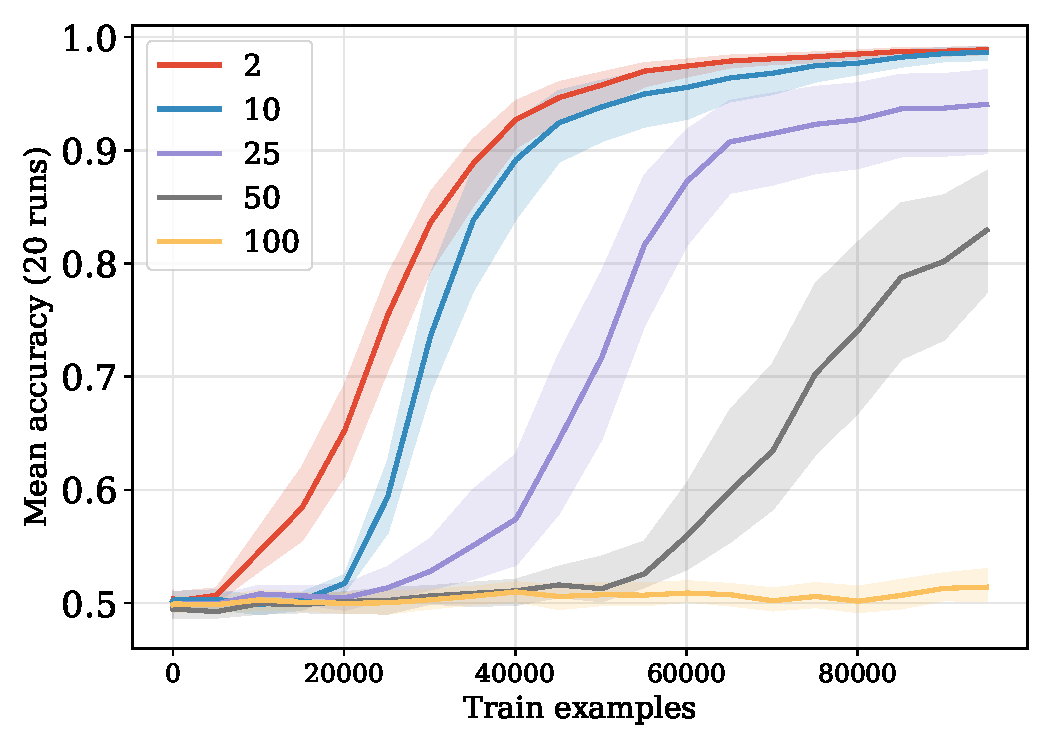
\includegraphics[width=1\textwidth]{../fig/flatpremack-h2-train_size-embed_dim-hidden_dim=10.pdf}
    \caption{Hidden dimensionality 10.}
  \end{subfigure}

  \vspace{24pt}

  \begin{subfigure}{0.45\linewidth}
    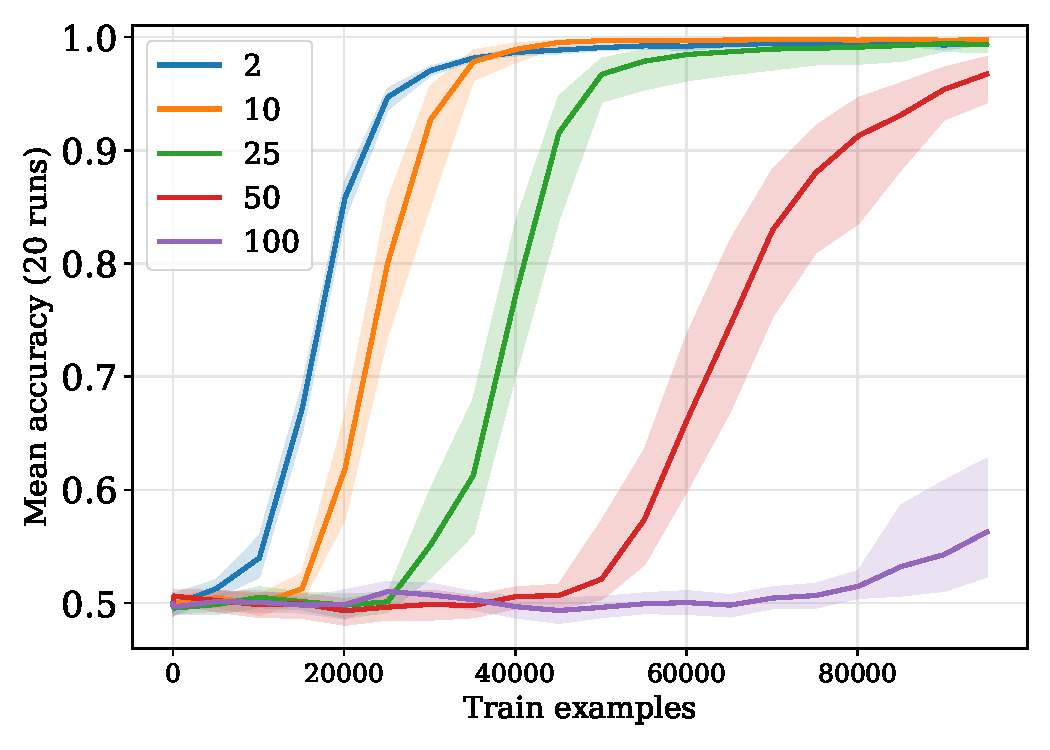
\includegraphics[width=1\textwidth]{../fig/flatpremack-h2-train_size-embed_dim-hidden_dim=25.pdf}
    \caption{Hidden dimensionality 25.}
  \end{subfigure}
  \hfill
  \begin{subfigure}{0.45\linewidth}
    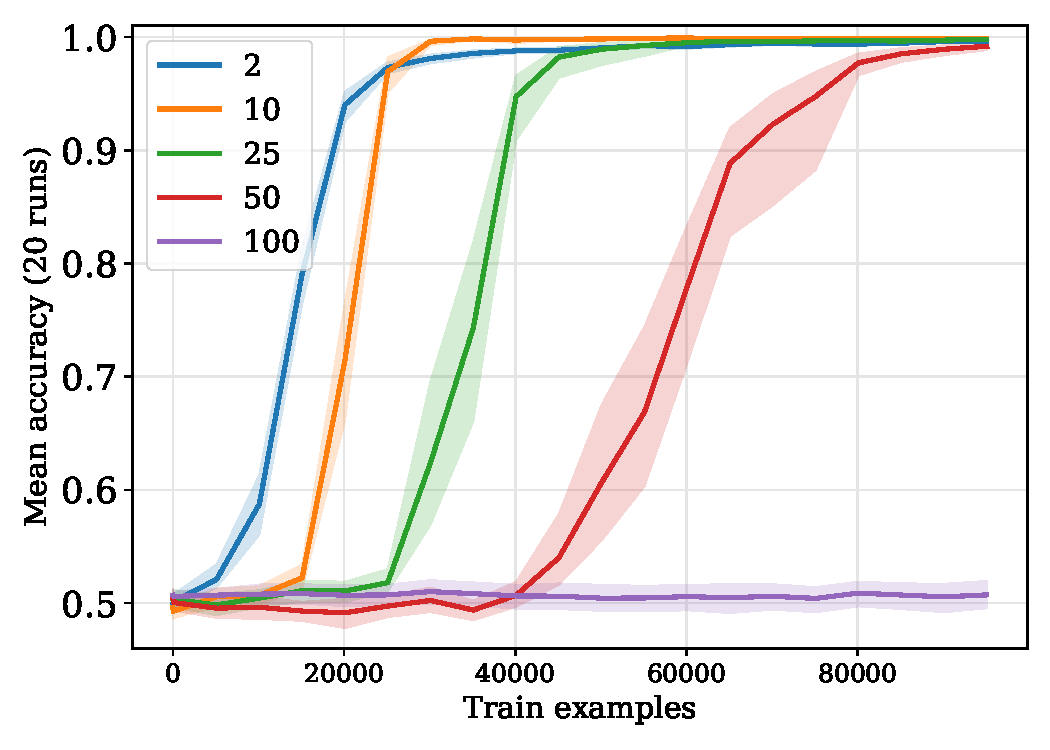
\includegraphics[width=1\textwidth]{../fig/flatpremack-h2-train_size-embed_dim-hidden_dim=50.pdf}
    \caption{Hidden dimensionality 50.}
  \end{subfigure}

  \vspace{24pt}

  \begin{subfigure}{0.45\linewidth}
    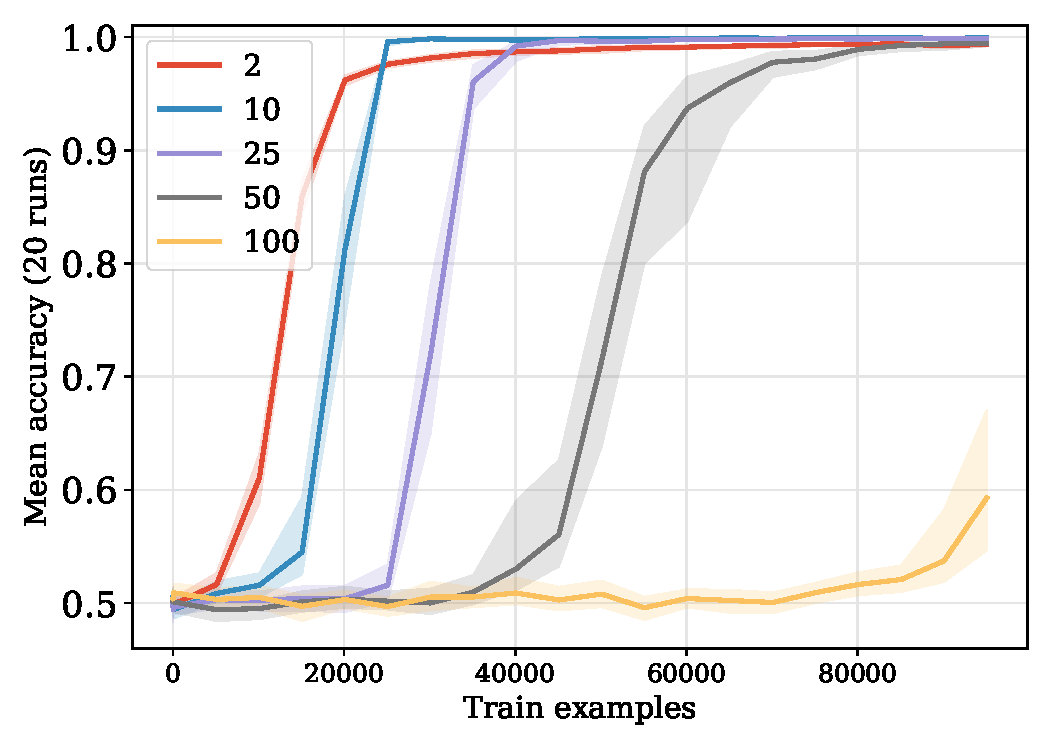
\includegraphics[width=1\textwidth]{../fig/flatpremack-h2-train_size-embed_dim-hidden_dim=100.pdf}
    \caption{Hidden dimensionality 100.}
    \label{fig:model3a-rep}
  \end{subfigure}
  \caption{Results for Model 3a applied to the hierarchical same--different task.}
  \label{fig:model3a}
\end{figure}

\newpage

\subsection{Pretraining input representations and equality parameters}\label{app:double-pretrain}

In \secref{sec:modular}, we showed that pretraining an entire basic equality network led to faster learning in the hierarchical same--different task. This kind of network pretraining can be combined with the input-level pretrained we explored elsewhere in the paper (details in \appref{app:pretraining}). \Figref{fig:double-pretrain} reports initial experiments for this combination of pretraining regimes. Although the results are not better than the ones we report in the paper, this still seems like a promising idea, though one for which optimal solutions might be hard to find.

\begin{figure}[H]
  \centering
  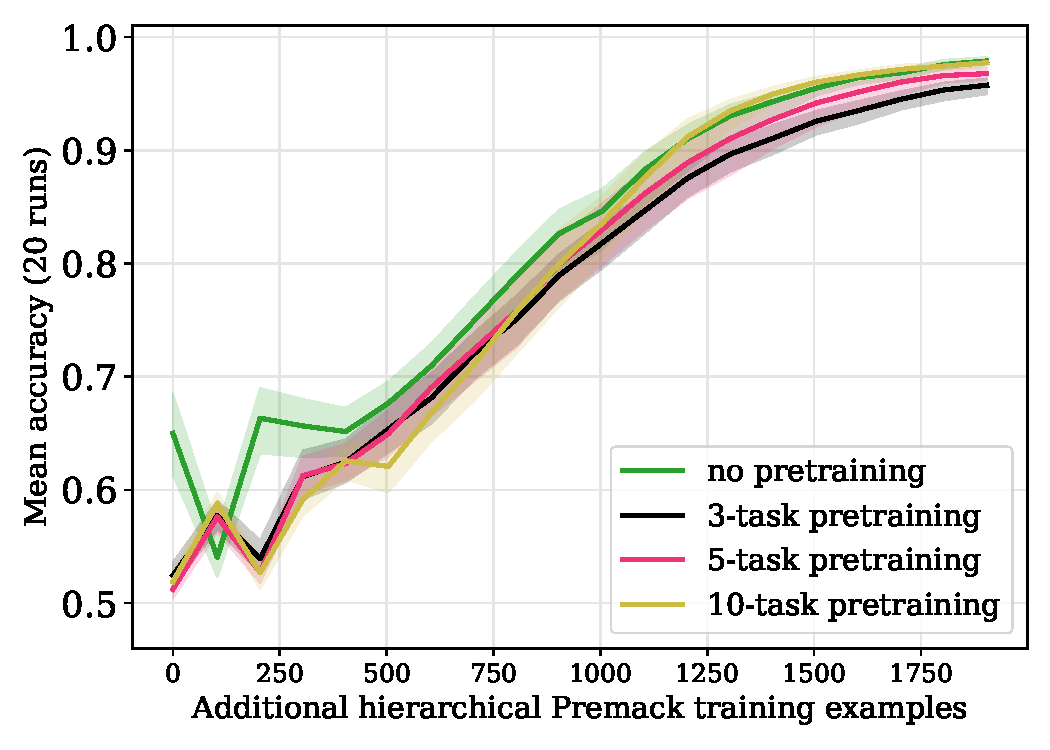
\includegraphics[width=0.48\textwidth]{../fig/input-as-output-pretrain-compare-train_size-pretrained-embed_dim=None.pdf}
  \caption{Results for the hierarchical same--different task for a model in which both the input representations and the basic equality network are pretrained. The `no pretrain' model is the best one from \figref{fig:premack-pretraining-results} (25-dimensional embeddings, 100-dimensional hidden representations). The input-pretrained models use this same configuration.}
  \label{fig:double-pretrain}
\end{figure}

\end{document}


\end{document}

}{
  \section*{Acknowledgements}

\update{This work is supported in part by a Facebook Robust Deep Learning for Natural Language Processing Research Award.}


\bibliographystyle{acl_natbib}
\bibliography{relational-learning-bib}

%\documentclass[9pt,twoside,lineno]{pnas-new}
% Use the lineno option to display guide line numbers if required.

\templatetype{pnassupportinginfo}

\title{Your main manuscript title}
\author{Author1, Author2 and Author3 (complete author list)}
\correspondingauthor{Corresponding Author name.\\E-mail: author.two@email.com}

\input{pre-macros}


\begin{document}

\maketitle

%% Adds the main heading for the SI text. Comment out this line if you do not have any supporting information text.
\SItext


% \appendix

\section{Model 1 Supplementary Methods}

The input to our model is a pair of vectors $(a, b)$, each of dimension $m$, which correspond to the two stimulus objects. These vectors are non-featural representations that do not have features encoding properties of the objects or their identity. These are concatenated to form a single vector $[a;b]$ of dimension $2m$, which is the simplest way of merging the two representations to form a single input.

This representation is multiplied by a matrix of weights $W_{xh}$ of dimension $2m \times n$ and a bias vector $b_{h}$ of dimension $n$ is added to this result, where $n$ is the hidden layer dimensionality. These two steps create a linear projection of the input representation, and the bias term is the value of this linear projection when the input representation is the zero vector. Then, the non-linear activation function $\ReLU$ ($\ReLU(x) = \max(0, x)$) is applied element-wise to this linear projection. This non-linearity is what gives the neural model more expressive power than a logistic regression \citep{Cybenko:1989,Hornik:Stinchcombe:White:1989}. The result is the hidden representation $h$.

The hidden representation is the input to the classification layer: $h$ is multiplied by a second matrix of weights $W_{hy}$, dimension $n \times 2$, and a bias term $b_{y}$ (dimension 2) is added to this. This second bias term encodes the probabilities of each class when the hidden representation is 0. The result is fed through the softmax activation function: $\softmax(x)_{i} = \frac{\exp{x_{i}}}{\sum_{j} \exp{x_{j}}}$. This creates a probability distribution over the classes (positive and negative). For a given input, the model computes this probability distribution and the input is categorized as the class with the higher probability.

During training, this model is presented with positive and negative labeled examples and the parameters $W_{xh}$, $W_{hy}$, $b_{y}$, and $b_{h}$ are learned using back propagation with a cross entropy function. \update{This function is defined as follows, for a set of $N$ examples and $K$ classes:
%
\begin{equation}
\max(\theta)
\quad
\frac{1}{N}
\sum_{i=1}^{N}
\sum_{k=1}^{K}
y^{i,k} \log(h_{\theta}(i)^{k})
\end{equation}
%
where $\theta$ abbreviates the model parameters ($W_{xh}$, $W_{hy}$, $b_{y}$, $b_{h}$), $y^{i,k}$ is the actual label for example $i$ and class $k$, and $h_{\theta}(i)^{k}$ is the corresponding prediction.}


\section{Model 2 Supplementary Methods}

The input to this model is a sequence of vectors $x_1, x_2, x_3, \dots$, each of dimension $m$, which correspond to a sequence of stimulus objects. These vectors are, again, non-featural representations that do not have features encoding properties of the objects or their identity.


At each timestep $t$, the input vector $x_t$ is fed into the $\LSTM$ cell along with the previous hidden representation $h_{t-1}$. The defining feature of an $\LSTM$ is the ability to decide whether to store information from the current input, $x_t$, and whether to remember or forget the information from the previous timestep $h_{t-t}$. The output of the $\LSTM$ cell is the hidden representation for the current time step $h_t$. The dimension of the hidden representations is $n$. The hidden representation is multiplied by a matrix $W$ with dimensionality $n \times m$ to produce $y_t$. This result, $y_t$, is a linear projection of the hidden representation into the input vector space, which is necessary because $y_t$ is a prediction of what the next input, $x_{t+1}$, will be.

% \update{
The objective function is as follows:
%
\begin{equation}
\max(\theta)
\quad
-\frac{1}{N}
\sum_{i=1}^{N}
\sum_{t=1}^{T_{i}}
\left\| h_{\theta}\left(x^{i, 0:{t-1}}\right) - x^{i,t} \right\|^{2}
\end{equation}
%
for $N$ examples. Here, $T_{i}$ is the length of example $i$. As before, $\theta$ abbreviates the parameters of the model as specified in \dasheg{eq:lstm-recur}{eq:lstm-predict}. We use $h_{\theta}(x^{i, 0:{t-1}})$ for the vector predicted by the model for example~$i$ at timestep~$t$, which is compared to the actual vector at timestep $t$ via squared Euclidean distance (i.e., the mean squared error).
% As noted above, this is an unusual formulation for a language model. The usual version essentially treats every timestep as involving a classification decision, with a cross-entropy loss. We cannot adopt this because of our goal of using unseen vocabulary items at test time. % MCF: seemed redundant


\section{Model figures}


\subsection{Model 1: Same--different relation with feed-foward  networks}\label{sec:model1}

Our model of equality is given by \dasheg{eq:x2h-supp}{eq:h2y-supp}:
%
\begin{align}
  h &= \ReLU([a;b]W_{xh} + b_{h}) \label{eq:x2h-supp}\\
  y &= \softmax(hW_{hy} + b_{y}) \label{eq:h2y-supp}
\end{align}
%
The input is a pair of vectors $(a,b)$, each of dimension $m$, which correspond to two stimulus objects. These vectors are non-featural representations that do not hav efeatures encoding properties of the objects or their identities. These are concatenated to form a single vector $[a;b]$ of dimension $2m$, which is the simplest way of merging the two representations to form a single input.

This representation is multiplied by a matrix of weights $W_{xh}$ of dimension $2m \times n$ and a bias vector $b_{h}$ of dimension $n$ is added to this result, where $n$ is the hidden layer dimensionality. These two steps create a linear projection of the input representation, and the bias term is the value of this linear projection when the input representation is the zero vector. Then, the non-linear activation function $\ReLU$ ($\ReLU(x) = \max(0, x)$) is applied element-wise to this linear projection. This non-linearity is what gives the neural model more expressive power than a logistic regression \citep{Cybenko:1989,Hornik:Stinchcombe:White:1989}. The result is the hidden representation $h$.

The hidden representation is the input to the classification layer: $h$ is multiplied by a second matrix of weights $W_{hy}$, dimension $n \times 2$, and a bias term $b_{y}$ (dimension 2) is added to this. This second bias term encodes the probabilities of each class when the hidden representation is 0. The result is fed through the softmax activation function: $\softmax(x)_{i} = \frac{\exp{x_{i}}}{\sum_{j} \exp{x_{j}}}$. This creates a probability distribution over the classes (positive and negative). For a given input, the model computes this probability distribution and the input is categorized as the class with the higher probability.

The parameters $W_{xh}$, $W_{hy}$, $b_{y}$, and $b_{h}$ are learned using back propagation with a cross entropy function. \update{This function is defined as follows, for a set of $N$ examples and $K$ classes:
%
\begin{equation}\label{eq:crossent}
\max(\theta)
\quad
\frac{1}{N}
\sum_{i=1}^{N}
\sum_{k=1}^{K}
y^{i,k} \log(h_{\theta}(i)^{k})
\end{equation}
%
where $\theta$ abbreviates the model parameters ($W_{xh}$, $W_{hy}$, $b_{y}$, $b_{h}$), $y^{i,k}$ is the actual label for example $i$ and class $k$, and $h_{\theta}(i)^{k}$ is the corresponding prediction.}

\Figref{fig:models:equality} provides a visual depiction of the model. The gray boxes correspond to embedding representations, the purple box is the hidden representation $h$, and the red box is the output distribution $y$. Dotted arrows depict concatenation, and solid arrows depict the dense relations corresponding to the matrix multiplications (plus bias terms) in \dasheg{eq:x2h}{eq:h2y}.

\begin{figure}[H]
  \centering
  \resizebox{100pt}{!}{%
    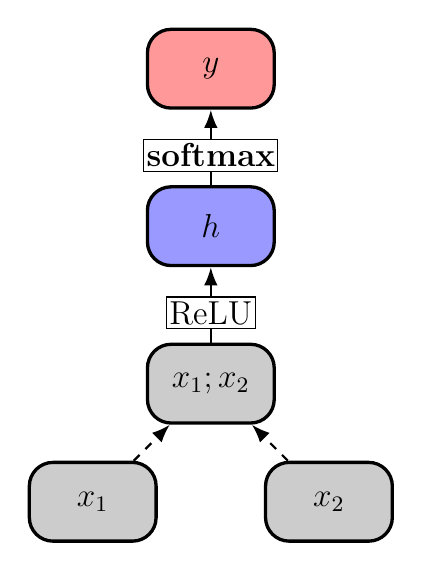
\begin{tikzpicture}[
      % GLOBAL CFG
      font=\sf \large,
      >=LaTeX,
      % Styles
      rep/.style={% For representations
        rectangle,
        rounded corners=3mm,
        draw,
        very thick,
        minimum height =1cm,
        minimum width=1.61cm
      },
      function/.style={%For functions
        ellipse,
        draw,
        inner sep=1pt
      },
      gt/.style={% For internal inputs
        rectangle,
        draw,
        minimum width=5mm,
        minimum height=4mm,
        inner sep=1pt
      },
      function/.style={
        rectangle,
        draw,
        minimum width=5mm,
        minimum height=4mm,
        inner sep=1pt
      },
      arrowconcat/.style={% Arrows for concatenation
        rounded corners=.25cm,
        dashed,
        thick,
        ->,
      },
      arrowfunction/.style={% Arrows for concatenation
        rounded corners=.25cm,
        thick,
        ->,
      }
      ]

      % Start drawing the thing...
      % Draw the cell:
      \node [rep, fill=\inputcolor] (input1) at (-1.5,1.5){$x_1$} ;
      \node [rep, fill=\inputcolor] (input2) at (1.5,1.5){$x_2$} ;
      \node [rep, fill=\inputcolor] (concat) at (0,3){$x_1;x_2$} ;
      \draw [arrowconcat] (input1) -- (concat);
      \draw [arrowconcat] (input2) -- (concat);


      \node [rep, fill=\hiddencolor] (hidden) at (0,5){$h$} ;
      \node [gt, minimum width=1cm] (relu) at (0,4-0.1) {$\ReLU$};
      \draw [arrowfunction] (concat) -- (relu) -- (hidden);


      \node [rep,fill=\outputcolor] (output) at (0,7){$y$} ;
      \node [gt, minimum width=1cm] (softmax) at (0,6-0.1) {$\softmax$};
      \draw [arrowfunction] (hidden) -- (softmax) -- (output);

    \end{tikzpicture}
  }
  \caption{A single layer network computing equality.}
  \label{fig:models:equality}
\end{figure}


\subsection{Model 2: Sequential same--different (ABA task)}\label{sec:model2}

The specific model we use for this is as follows:
%
\begin{align}
  h_{t} &= \LSTM(x_{t}, h_{t-1}) \label{eq:lstm-recur-supp}\\
  y_{t} &= h_{t}W + b\label{eq:lstm-predict-supp}
\end{align}
%
This holds for $t > 0$, and we set $h_{0} = \mathbf{0}$. $\LSTM$ is a long short-term memory cell \cite{hochreiter:1997}. Full details on these cells are given in \appref{sec:analyticlm}.

The input is a sequence of vectors $x_1, x_2, x_3, \dots$, each of dimension $m$, which correspond to a sequence of stimulus objects. These vectors are, again, non-featural representations that do not have features encoding properties of the objects or their identity.

At each timestep $t$, the input vector $x_t$ is fed into the $\LSTM$ cell along with the previous hidden representation $h_{t-1}$. The defining feature of an $\LSTM$ is the ability to decide whether to store information from the current input, $x_t$, and whether to remember or forget the information from the previous timestep $h_{t-t}$. The output of the $\LSTM$ cell is the hidden representation for the current time step $h_t$. The dimension of the hidden representations is $n$. The hidden representation is multiplied by a matrix $W$ with dimensionality $n \times m$ to produce $y_t$. This result, $y_t$, is a linear projection of the hidden representation into the input vector space, which is necessary because $y_t$ is a prediction of what the next input, $x_{t+1}$, will be.

The objective function is as follows:
%
\begin{equation}
\max(\theta)
\quad
-\frac{1}{N}
\sum_{i=1}^{N}
\sum_{t=1}^{T_{i}}
\left\| h_{\theta}\left(x^{i, 0:{t-1}}\right) - x^{i,t} \right\|^{2}
\end{equation}
%
for $N$ examples. Here, $T_{i}$ is the length of example $i$. As before, $\theta$ abbreviates the parameters of the model as specified in \dasheg{eq:lstm-recur-supp}{eq:lstm-predict-supp}. We use $h_{\theta}(x^{i, 0:{t-1}})$ for the vector predicted by the model for example~$i$ at timestep~$t$, which is compared to the actual vector at timestep $t$ via squared Euclidean distance (i.e., the mean squared error).

\Figref{fig:reps:sequence} depicts this model. At each timestep $t$, a vector $y_{t}$ (red) is predicted based on the input representation at $t$ (gray) and the hidden representation at $t$ (purple). During training, this is compared with the actual vector for timestep $t+1$ (green). During testing, the predicted vector $y_{i}$ is compared with every item in the union of the train and assessment vocabularies, and the closest vector (according to Euclidean distance) is taken to be the prediction. This vector is then used as the input for timestep $t+1$.

\begin{figure}[H]
  \centering
  \resizebox{240pt}{!}{%
    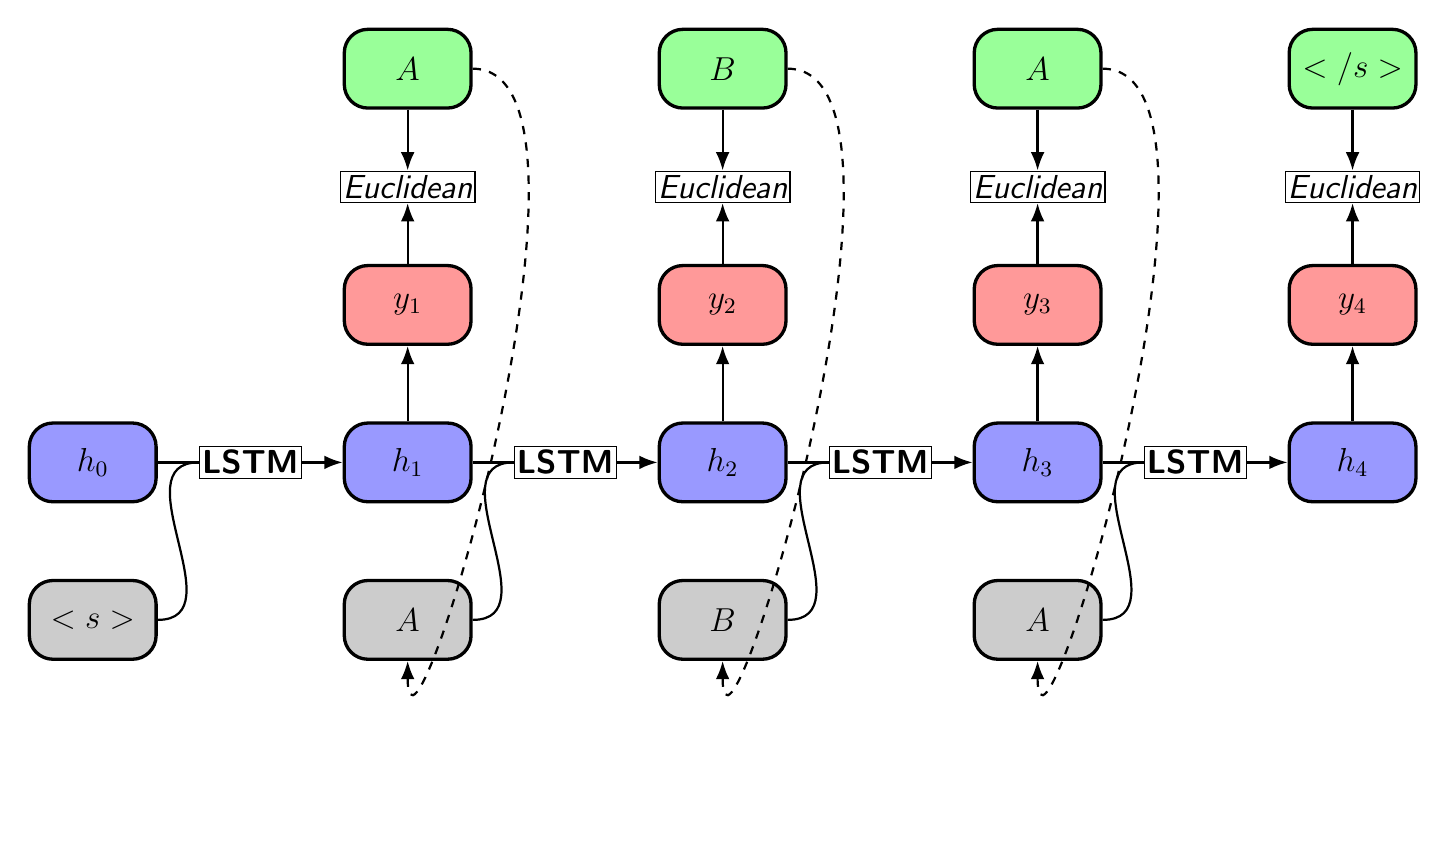
\begin{tikzpicture}[
      % GLOBAL CFG
      font=\sf \large,
      >=LaTeX,
      % Styles
      rep/.style={% For representations
        rectangle,
        rounded corners=3mm,
        draw,
        very thick,
        minimum height =1cm,
        minimum width=1.61cm
      },
      function/.style={%For functions
        ellipse,
        draw,
        inner sep=1pt
      },
      gt/.style={% For internal inputs
        rectangle,
        draw,
        minimum width=5mm,
        minimum height=4mm,
        inner sep=1pt
      },
      function/.style={
        rectangle,
        draw,
        minimum width=5mm,
        minimum height=4mm,
        inner sep=1pt
      },
      arrowconcat/.style={% Arrows for concatenation
        rounded corners=.25cm,
        dashed,
        thick,
        ->,
      },
      arrowfunction/.style={% Arrows for concatenation
        rounded corners=.25cm,
        thick,
        ->,
      }
      ]

      % Start drawing the thing...
      % Draw the cell:
      \node [rep, fill=\inputcolor] (input1) at (-10,4){$<s>$} ;
      \node [rep, fill=\inputcolor] (input2) at (-6,4){$A$} ;
      \node [rep, fill=\inputcolor] (input3) at (-2,4){$B$} ;
      \node [rep, fill=\inputcolor] (input4) at (2,4){$A$} ;

      \node [rep, fill=\hiddencolor] (hidden0) at (-10,6){$h_0$} ;
      \node [rep, fill=\hiddencolor] (hidden1) at (-6,6){$h_1$} ;
      \node [rep, fill=\hiddencolor] (hidden2) at (-2,6){$h_2$} ;
      \node [rep, fill=\hiddencolor] (hidden3) at (2,6){$h_3$} ;
      \node [rep, fill=\hiddencolor] (hidden4) at (6,6){$h_4$} ;

      \node [gt] (LSTM0) at (-8,6){$\LSTM$} ;
      \node [gt] (LSTM1) at (-4,6){$\LSTM$} ;
      \node [gt] (LSTM2) at (0,6){$\LSTM$} ;
      \node [gt] (LSTM3) at (4,6){$\LSTM$} ;

      \node [rep, fill=\outputcolor] (output1) at (-6,8){$y_1$} ;
      \node [rep, fill=\outputcolor] (output2) at (-2,8){$y_2$} ;
      \node [rep, fill=\outputcolor] (output3) at (2,8){$y_3$} ;
      \node [rep, fill=\outputcolor] (output4) at (6,8){$y_4$} ;

      \node [gt] (compare1) at (-6,9.5){$\compare$} ;
      \node [gt] (compare2) at (-2,9.5){$\compare$} ;
      \node [gt] (compare3) at (2,9.5){$\compare$} ;
      \node [gt] (compare4) at (6,9.5){$\compare$} ;

      \node [rep, fill=\colorlabel] (label1) at (-6,11){$A$} ;
      \node [rep, fill=\colorlabel] (label2) at (-2,11){$B$} ;
      \node [rep, fill=\colorlabel] (label3) at (2,11){$A$} ;
      \node [rep, fill=\colorlabel] (label4) at (6,11){$</s>$} ;

      \draw [arrowfunction] (label1) -- (compare1);
      \draw [arrowfunction] (label2) -- (compare2);
      \draw [arrowfunction] (label3) -- (compare3);
      \draw [arrowfunction] (label4) -- (compare4);

      \draw [arrowfunction] (output1) -- (compare1);
      \draw [arrowfunction] (output2) -- (compare2);
      \draw [arrowfunction] (output3) -- (compare3);
      \draw [arrowfunction] (output4) -- (compare4);

      \draw [arrowfunction] (hidden1) -- (output1);
      \draw [arrowfunction] (hidden2) -- (output2);
      \draw [arrowfunction] (hidden3) -- (output3);
      \draw [arrowfunction] (hidden4) -- (output4);

      \draw [thick] (input1) to[out=0,in=-180, distance=1cm] (LSTM0);
      \draw [thick] (input2) to[out=0,in=-180, distance=1cm] (LSTM1);
      \draw [thick] (input3) to[out=0,in=-180, distance=1cm] (LSTM2);
      \draw [thick] (input4) to[out=0,in=-180, distance=1cm] (LSTM3);

      \draw [arrowfunction] (hidden0) -- (LSTM0) -- (hidden1);
      \draw [arrowfunction] (hidden1) -- (LSTM1)-- (hidden2);
      \draw [arrowfunction] (hidden2) -- (LSTM2)-- (hidden3);
      \draw [arrowfunction] (hidden3) -- (LSTM3)-- (hidden4);

      \draw[->,dashed,thick] (label1) to[out=0,in=-90, distance=1.99cm] (input2);
      \draw[->,dashed,thick] (label2) to[out=0,in=-90, distance=1.99cm] (input3);
      \draw[->,dashed,thick] (label3) to[out=0,in=-90, distance=1.99cm] (input4);
    \end{tikzpicture}
  }
  \caption{A recursive LSTM network producing ABA sequences.}
  \label{fig:reps:sequence}
\end{figure}

\subsection{Model 3a: A single layer feed forward network }
 The only change required to equations \dasheg{eq:x2h-supp}{eq:h2y-supp} is that we create inputs $[a;b;c;d]$: the flat concatenation of all the elements of the two pair of vectors. This change in turn leads $W_{xh}$ to have dimensionality $4m \times n$. The objective function is again defined using a cross entropy function, as in equation \ref{eq:crossent}. \Appref{app:model1-premack} provides a full picture of these learning trends. These models are able to find nearly perfect solutions, but vastly more training data is required for this task than was required for simple equality, and the network configuration matters much more. For example, our model with 10-dimensional entity representations and 100-dimensional hidden representations reached near perfect accuracy, but only with over 95,000 training instances. A comparable model with 50-dimensional entity representations failed to get traction at all with this amount of training data, and pretraining led to only minor improvements. For this reason, we also perform experiments with a deeper neural network.


\subsection{Model 3b: A deeper feed-forward network for hierarchical same--different}\label{sec:model3a}

This model extends \dasheg{eq:x2h-supp}{eq:h2y-supp} with an additional hidden layer and a larger input dimensionality, corresponding to the input pair of pairs $((a,b), (c,d))$ being flattened into a single concatenated representation $[a;b;c;d]$:
%
\begin{align}
  h_{1} &= \ReLU([a;b;c;d]W_{xh} + b_{h_{1}}) \label{eq:x2h1-supp}\\
  h_{2} &= \ReLU(h_{1}W_{hh} + b_{h_{2}}) \label{eq:x2h2-supp}\\
  y &= \softmax(h_{2}W_{hy} + b_{y}) \label{eq:h2y2-supp}
\end{align}
%
The objective function is again defined using a cross entropy function, as in equation \ref{eq:crossent}.

\Figref{fig:models:premack-deep} depicts this model.

\begin{figure}[H]
  \centering
  \resizebox{150pt}{!}{%
    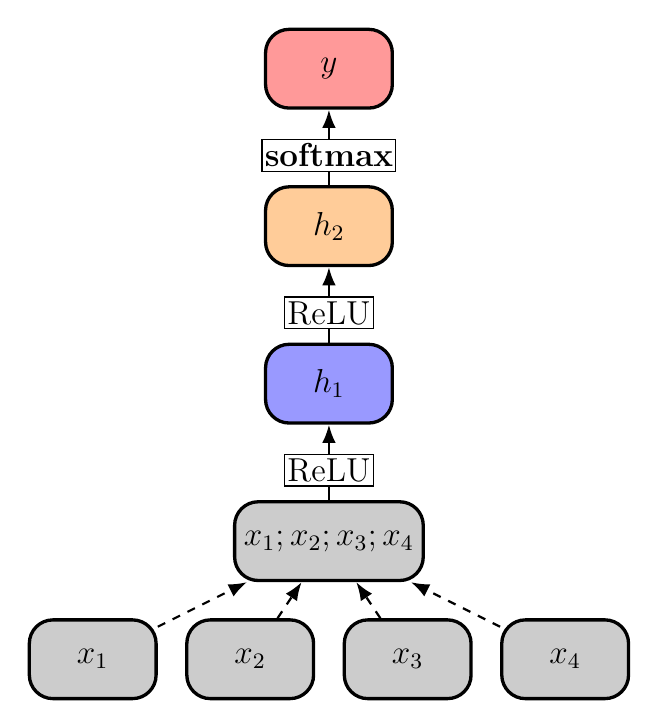
\begin{tikzpicture}[
      % GLOBAL CFG
      font=\sf \large,
      >=LaTeX,
      % Styles
      rep/.style={% For representations
        rectangle,
        rounded corners=3mm,
        draw,
        very thick,
        minimum height =1cm,
        minimum width=1.61cm
      },
      function/.style={%For functions
        ellipse,
        draw,
        inner sep=1pt
      },
      gt/.style={% For internal inputs
        rectangle,
        draw,
        minimum width=5mm,
        minimum height=4mm,
        inner sep=1pt
      },
      function/.style={
        rectangle,
        draw,
        minimum width=5mm,
        minimum height=4mm,
        inner sep=1pt
      },
      arrowconcat/.style={% Arrows for concatenation
        rounded corners=.25cm,
        dashed,
        thick,
        ->,
      },
      arrowfunction/.style={% Arrows for concatenation
        rounded corners=.25cm,
        thick,
        ->,
      }
      ]

      % Start drawing the thing...
      % Draw the cell:
      \node [rep, fill=\inputcolor] (input1) at (-3,1.5){$x_1$} ;
      \node [rep, fill=\inputcolor] (input2) at (-1,1.5){$x_2$} ;
      \node [rep, fill=\inputcolor] (input3) at (1,1.5){$x_3$} ;
      \node [rep, fill=\inputcolor] (input4) at (3,1.5){$x_4$} ;
      \node [rep, fill=\inputcolor] (concat) at (0,3){$x_1;x_2;x_3;x_4$} ;
      \draw [arrowconcat] (input1) -- (concat);
      \draw [arrowconcat] (input2) -- (concat);
      \draw [arrowconcat] (input3) -- (concat);
      \draw [arrowconcat] (input4) -- (concat);


      \node [rep, fill=\hiddencolor] (hidden) at (0,5){$h_1$} ;
      \node [gt, minimum width=1cm] (relu) at (0,4-0.1) {$\ReLU$};
      \draw [arrowfunction] (concat) -- (relu) -- (hidden);

      \node [rep, fill=\hiddencolortwo] (hidden2) at (0,7){$h_2$} ;
      \node [gt, minimum width=1cm] (relu2) at (0,6-0.1) {$\ReLU$};
      \draw [arrowfunction] (hidden) -- (relu2) -- (hidden2);


      \node [rep,fill=\outputcolor] (output) at (0,9){$y$} ;
      \node [gt, minimum width=1cm] (softmax) at (0,8-0.1) {$\softmax$};
      \draw [arrowfunction] (hidden2) -- (softmax) -- (output);

    \end{tikzpicture}
  }
  \caption{A two layer network computing hierarchical equality.}
  \label{fig:models:premack-deep}
\end{figure}


\subsection{Model 3c: Pretraining for hierarchical same--different}\label{sec:model3b}

Our pretraining model is as follows:
%
\begin{align}
  h_1 &= \ReLU([a;b]W_{xh} + b_{h}) \label{eq:preh1-supp}\\
  h_2 &= \ReLU([c;d]W_{xh} + b_{h})\\
  h_3 &= \ReLU([h_1;h_2]W_{xh} + b_{h}) \\
  y &= \softmax(h_3W_{hy} + b_{y}) \label{eq:prey-supp}\
\end{align}
%
where $W_{xh}$, $W_{hy}$, $b_h$, and $b_y$ are the parameters from the model in equations \dasheg{eq:x2h-supp}{eq:h2y-supp} already trained on basic equality. Crucially, the same parameters, $W_{xh}$ and $b_h$, are used three times: twice to compute representations encoding whether a pair of input entities are equal ($h_1$, $h_2$), and once to compute a representation ($h_{3}$) encoding whether the truth values encoded by $h_1$ and $h_2$ are equal. This final representation is then used to compute a probability distribution over two classes, and the class with the higher probability is predicted by the model.

The objective function is again defined using a cross entropy function, as in equation \ref{eq:crossent}.

\begin{figure}[H]
  \centering
  \resizebox{240pt}{!}{%
    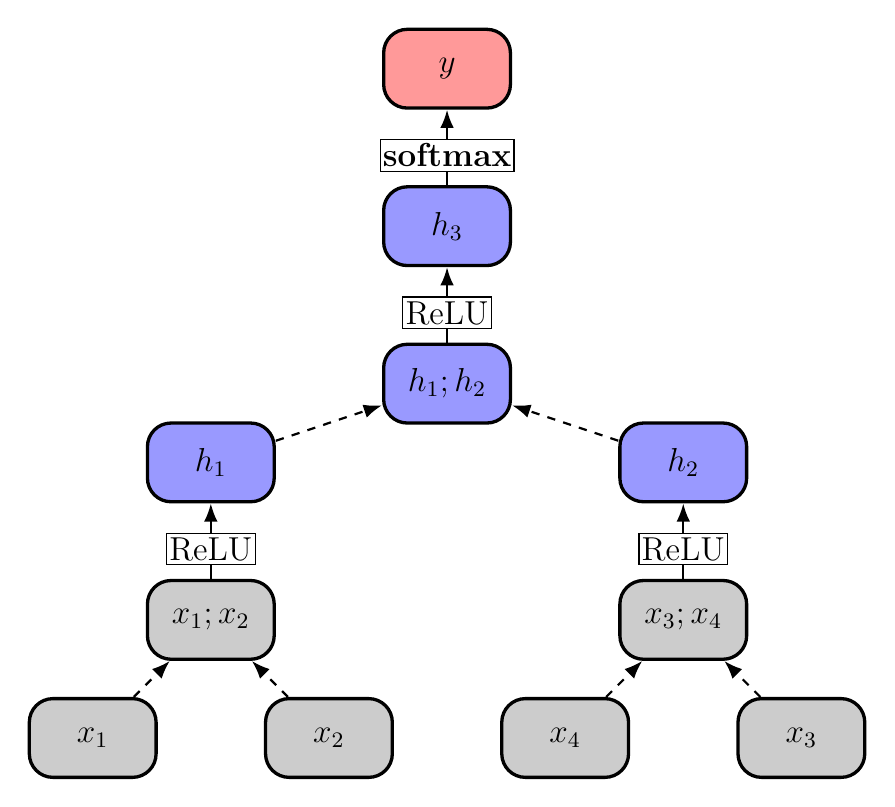
\begin{tikzpicture}[
      % GLOBAL CFG
      font=\sf \large,
      >=LaTeX,
      % Styles
      rep/.style={% For representations
        rectangle,
        rounded corners=3mm,
        draw,
        very thick,
        minimum height =1cm,
        minimum width=1.61cm
      },
      function/.style={%For functions
        ellipse,
        draw,
        inner sep=1pt
      },
      gt/.style={% For internal inputs
        rectangle,
        draw,
        minimum width=5mm,
        minimum height=4mm,
        inner sep=1pt
      },
      function/.style={
        rectangle,
        draw,
        minimum width=5mm,
        minimum height=4mm,
        inner sep=1pt
      },
      arrowconcat/.style={% Arrows for concatenation
        rounded corners=.25cm,
        dashed,
        thick,
        ->,
      },
      arrowfunction/.style={% Arrows for concatenation
        rounded corners=.25cm,
        thick,
        ->,
      }
      ]

      % Start drawing the thing...
      % Draw the cell:
      \node [rep, fill=\inputcolor] (input1) at (-4.5,1.5){$x_1$} ;
      \node [rep, fill=\inputcolor] (input2) at (-1.5,1.5){$x_2$} ;
      \node [rep, fill=\inputcolor] (concat) at (-3,3){$x_1;x_2$} ;
      \draw [arrowconcat] (input1) -- (concat);
      \draw [arrowconcat] (input2) -- (concat);


      \node [rep, fill=\hiddencolor] (hidden) at (-3,5){$h_1$} ;
      \node [gt, minimum width=1cm] (relu1) at (-3,4-0.1) {$\ReLU$};
      \draw [arrowfunction] (concat) -- (relu1) -- (hidden);


      \node [rep, fill=\inputcolor] (input3) at (4.5,1.5){$x_3$} ;
      \node [rep, fill=\inputcolor] (input4) at (1.5,1.5){$x_4$} ;
      \node [rep, fill=\inputcolor] (concat2) at (3,3){$x_3;x_4$} ;
      \draw [arrowconcat] (input3) -- (concat2);
      \draw [arrowconcat] (input4) -- (concat2);


      \node [rep, fill=\hiddencolor] (hidden2) at (3,5){$h_2$} ;
      \node [gt, minimum width=1cm] (relu2) at (3,4-0.1) {$\ReLU$};
      \draw [arrowfunction] (concat2) -- (relu2) -- (hidden2);


      \node [rep,fill=\hiddencolor] (hiddenconcat) at (0,6){$h_1;h_2$};
      \draw [arrowconcat] (hidden2) -- (hiddenconcat);
      \draw [arrowconcat] (hidden) -- (hiddenconcat);


      \node [rep, fill=\hiddencolor] (hidden3) at (0,8){$h_3$} ;
      \node [gt, minimum width=1cm] (relu3) at (0,7-0.1) {$\ReLU$};
      \draw [arrowfunction] (hiddenconcat) -- (relu3) -- (hidden3);


      \node [rep,fill=\outputcolor] (output) at (0,10){$y$} ;
      \node [gt, minimum width=1cm] (softmax) at (0,9-0.1) {$\softmax$};
      \draw [arrowfunction] (hidden3) -- (softmax) -- (output);

    \end{tikzpicture}
  }
  \caption{A single layer network pretrained on equality computing hierarchical equality.}
  \label{fig:models:premack}
\end{figure}


\section{Pretraining}\label{app:pretraining}

Our pretraining model closely resembles the models used for our main experiments. It defines a feed-forward network with a multitask objective. For an example $i$ and task $j$:
%
\begin{align}
  h_{i} &= \ReLU\left( E[i]W_{xh} + b_{h} \right) \\
  y_{i,j} &= \softmax(h^{i}W_{hy}^{j} + b_{y}^{j})
\end{align}
%
where $E[i]$ is the vector representation for example $i$ in the embedding matrix $E$. The overall objective of the model is to maximize the sum of the task objective functions. For $N$ examples, $J$ tasks, and $K_{j}$ the number of classes for task $j$:
%
\begin{equation}
  \max(\theta)
  \quad
  \frac{1}{N}
  \sum_{i=1}^{N}
  \sum_{j=1}^{J}
  \sum_{k=1}^{K_{j}}
  y^{i,j,k} \log \left( h_{\theta}(i)^{j,k} \right)
\end{equation}
%
where $y^{i,j,k}$ is the correct label for example $i$ in task $j$ and $p^{i,j,k}$ is the predicted value for example $i$ in task $j$.

For the experiments in the paper, we initialize $E$ randomly and then, for pretraining on $J$ tasks, we create a random binary vector of length $J$ for each row in $E$. Each dimension (task) in $J$ is independent of the others.

Our motivation for pretraining is to update the embedding $E$ so that its representations contain rich structure that can be used by subsequent models. To achieve this, we backpropagate errors through the network and into $E$.

In our experiments, we always pretrain for 10 iterations. This choice is motivated primarily by computational costs; additional pretraining iterations greatly increase experiment run-times, though they do have the potential to imbue the representations with even more useful structure.


\section{Model optimization details}\label{app:optimization}

The feed forward networks for basic and hierarchical equality were implemented using the multi-layer perception from sklearn and a cross entropy function was used to compute the prediction error. The recursive LSTM network for the sequential ABA task was implemented using PyTorch and a mean squared error function was used to compute the prediction error. The networks for pretraining representations and for the hierarchical equality task were also implemented using PyTorch, with cross-entropy loss functions used to compute the prediction errors. For all models, Adam optimizers \citep{Kingma:Ba:2015} were used. For all models, a hyperparameter search was run over learning rate values of \{0.00001, 0.0001, 0.001\} and l2 normalization values of \{0.0001, 0.001, 0.01\} for each hidden dimension and input dimension mentioned in the paper.


\section{Localist and binary feature representations prevent generalization}\label{app:generalization}

The method of representation impacts whether there is a natural notion of similarity between entities and the ability of models to generalize to examples unseen in training. These two attributes are deeply related; if there is a natural notion of similarity between vector representations, then models can generalize to inputs with representations that are similar to those seen in training.

In order to discuss how representation impacts generalization, we will need explain some properties of how neural models are trained. Standard neural models, including all models in the paper, begin with applying a linear layer to the input vector where no two input units are connected to the same weight. An easily observed fact about the back-propagation learning algorithm is that, if a unit of the input vector is always zero during training, then any weights connected to that unit and only that unit will not change from their initialized values during training. This means that, when a standard neural model is evaluated on an input vector that has a non-zero value for a unit that was zero throughout training, untrained weights are used and behavior is unpredictable.

Localist representations are orthogonal and equidistant from one another so there is no notion of similarity and consequently standard neural models have no ability to generalize to new examples. No two representations share a non-zero unit, and so when models are presented with inputs unseen in training, untrained weights are used and the resulting behavior is again unpredictable.

Distributed representations with binary features also limit generalization, though less severely than localist representations. Localist representations prevent generalization to entities unseen during training, while binary feature representations prevent generalization to features unseen during training. For example, if color and shape are represented as binary features, and a red square and blue circle are seen in training, then a model could generalize to the unseen entities of a blue circle or a red square. However, if no entity that is a circle is seen during training, then the binary feature representing the property of being a circle is zero throughout training and untrained weights are used when the model is presented with a entity that is a circle during testing, which results in unpredictable behavior.

Distributed representations with analog features do not inhibit generalization in the same way. If height is represented as a binary feature, then a single unit represents all height values and is always non-zero. Non-featural representations similarly do not inhibit generalization, because all units for all representations are non-zero and the network can learn parameters that create complex associations between these entities and its task labels.


\section{An analytic solution to identity with a feed forward network}\label{app:equality-solution}

We now show that our feed forward networks can solve the same--different problem we pose, in the following sense: for any set of inputs, we can find parameters $\theta$ that perfectly classify those inputs. At the same time, we also show that there are always additional inputs for which $\theta$ makes incorrect predictions.

Here are the parameters of a feed forward neural network that performs a binary classification task
%
\[ \texttt{ReLu}(\begin{pmatrix} x_1 \\ x_2  \end{pmatrix}^T \begin{pmatrix} W^{11} & W^{12}\\ W^{21}& W^{22} \end{pmatrix}) \begin{pmatrix} v^{11} & v^{12} \\ v^{21} & v^{22} \end{pmatrix} + \begin{pmatrix}b_1 &b_2 \end{pmatrix}= \begin{pmatrix} o_1 & o_2\end{pmatrix}\]
%
where, if $n$ is the dimension of entity embeddings used, then
%
\begin{align*}
  x, y,v^{11}, v^{12}, v^{21}, v^{22} &\in \mathbb{R}^{n \times 1} \\
  W^{11}, W^{12},W^{21}, W^{22} &\in \mathbb{R}^{n \times n} \\
  b_1, b_2, o_1, o_2 &\in \mathbb{R}
\end{align*}
%
Given an input $(x_1,x_2)$, if the output $o_1$ is larger than $o_2$, then one class is predicted; if the output $o_2$ is larger that $o_1$, then the other class is predicted. When the two outputs are equal, the network has predicted that both classes are equally likely and we can arbitrarily decide which class is predicted. In this case, the output $o_1$ predicts the two inputs, $x_1$ and $x_2$, are in the identity relation and the output $o_2$ predicts the two inputs are not. Now we specify parameters to provide an analytic solution to the identity relation using this network
%
\[ \texttt{ReLu}(\begin{pmatrix} x_1 \\ x_2 \end{pmatrix}^T \begin{pmatrix} I & -I\\ -I& I \end{pmatrix}) \begin{pmatrix} \vec{1} & \vec{0} \\ \vec{1} & \vec{0} \end{pmatrix} + \begin{pmatrix}b_1 &b_2 \end{pmatrix}= \begin{pmatrix} o_1 & o_2\end{pmatrix}\]
%
where $I$ is the identity matrix, $-I$ is the negative identity matrix, and $\vec{1}$ and $\vec{0}$ are the two vectors in $\mathbb{R}^n$ that have all zeros and all ones, respectively. The output values, given an input, are
%
\[ o_1 = \sum_{i = 1}^{n}|(x_1)_i- (x_2)_i|+ b_1 \qquad \quad  o_2 = b_2\]
%
where two parameters are left unspecified, $b_1, b_2$. We present a visualization in Figure~\ref{fig:analyticff} of how the analytic solution to identity of this network changes depending on the values of two bias terms. In this example, the network receives two one-dimensional inputs, $x_1$ and $x_2$. If the ordered pair of inputs is in the shaded area on the graph, then they are predicted to be in the identity relation. If in the unshaded area, they are predicted not to be. The dotted line is where the network predicts the two classes to be equally likely.


\begin{figure}[h]
  \centering
  \newcommand\X{2}
  \newcommand\E{0.03}
  % \tcbox{
  \begin{tikzpicture}[scale=0.7]
    \centering
    \filldraw[fill=black, opacity=0.1]
    (-5,-5 + \X)--(5-\X,5) -- (5,5) -- (5,5 - \X)--(-5+ \X,-5)--(-5,-5)--(-5,-5 + \X);
    \draw[<->,ultra thick] (-5,0)--(5,0) node[right]{$x_1$};
    \draw[<->,ultra thick] (0,-5)--(0,5) node[above]{$x_2$};
    \draw[<->,thick] (-5,-5)--(5,5) ;
    \draw[<->,thick, dashed] (-5,-5 + \X)--(5-\X,5) ;
    \draw[<->,thick,dashed] (-5+ \X,-5)--(5,5 - \X) ;
    \draw [decorate,decoration={brace,amplitude=12pt},xshift=-0pt,yshift=0pt]
    (3 - \X/2 + \E ,3 + \X/2- \E) -- (3-\E,3+\E) node [black,midway, xshift=12pt,yshift=12pt]
    { \rotatebox{-45}{$\scriptstyle b_1 - b_2$}};
  \end{tikzpicture}
  % }
  \caption{A visual representation of how the analytic solution to identity of a single layer feed forward network changes depending on the values of two bias terms, $b_1,b_2$.}
  \label{fig:analyticff}
\end{figure}

The network predicts $x_1$ and $x_2$ to be in the identity relation if $\sum_{i = 1}^{n}|x_i- y_i| < b_1-b_2$ which is visualized as the points between two parallel lines above and below the solution line $x_1 = x_2$. As the difference $b_1-b_2$ gets smaller and smaller, the two lines that bound the network's predictions get closer and closer to the solution line. However, as long as $b_1-b_2$ is positive, there will always be inputs of the form $(r,r+(b_1-b_2)/2)$ that are false positives. For any set of inputs, we can find bias values that result in the network correctly classifying those inputs, but for any bias values, we can find an input that is incorrectly classified by those values. In other words, we have an arbitrarily good solution that is never perfect. We provide a proof below that there is no perfect solution and so this is the best outcome possible. However, if we were to decide that, if the network predicts that an input is equally likely in either class, then this input is predicted to be in the identity relation, we could have a perfect solution with $b_1= b_2$.

Here is proof that a perfect solution is not possible. A basic fact from topology is that the set $\{x: f(x) < g(x)\}$ is an open set if $f$ and $g$ are continuous functions. Let $N_{o_1}$ and $N_{o_2}$ be the functions that map an input $(x_1,x_2)$ to the output values of the neural network, $o_1$ and $o_2$, respectively. These functions are continuous. Consequently, the set $C = \{(x_1,x_2): N_{o_2}(x_1,x_2) < N_{o_1}(x_1,x_2)\}$, which is the set of inputs that are predicted to be in the equality relation, is open.

With this fact, we can show that, if the neural network correctly classifies any point on the solution line $x_1 = x_2$, then it must incorrectly classify some point not on the solution line. Suppose that $C$ contains some point $(x,x)$. Then, by the definition of an open set, $C$ contains some $\epsilon$ ball around $(x,x)$, and therefore $C$ contains $(x,x+\epsilon)$, which is not on the solution line $x_1=x_2$. Thus, $C$ can never be equal to the set $\{(x_1,x_2):x_1=x_2\}$. So, because $C$ is the set of inputs classified as being in the equality relation by the neural network, a perfect solution cannot be achieved. Thus, we can conclude our arbitrarily good solution is the best we can do.


\section{An analytic solution to ABA sequences}\label{sec:analyticlm}


Here are the parameters of a long short term memory recursive neural network (LSTM):
%
\begin{align*}
  f_t &= \sigma(x_t W_f  + h_{t-1} U_f  + b_f) \\
  i_t &= \sigma(x_t W_i  + h_{t-1} U_i + b_i) \\
  o_t &= \sigma(x_t W_o +  h_{t-1} U_o + b_o)\\
  c_t &= f_t \circ c_{t-1} + i_t \circ \ReLU(x_tW_c + h_{t-1}U_c + b_c) \\
  h_t &= o_t \circ \ReLU(c_t) \\
  y_t &= h_tV
\end{align*}
%
where, if $n$ is the representation size and $d$ is the network hidden dimension, then
%
\begin{align*}
  x_t \in \mathbb{R}^n, f_t, i_t, o_t,  h_t, c_t &\in \mathbb{R}^d\\
  W \in \mathbb{R}^{n \times d}, U &\in \mathbb{R}^{d \times d}\\
  V \in \mathbb{R}^{d \times n}, b &\in \mathbb{R}^d
\end{align*}
%
and $\sigma$ is the sigmoid function. The initial hidden state $h_0$ and initial cell state $c_0$ are both set to be the zero vector. We say that an LSTM model with specified parameters has learned to produce ABA sequences if the following holds: when the network is seeded with some entity vector representation as its first input, $x_1$, then the output $y_1$ is not equal to $x_1$ and at the next time step the output $y_2$ is equal to $x_1$.

We let $d = 2n + 1$ and assign the following parameters, which provide an analytic solution to producing ABA sequences:
%
\begin{align*}
  f_t &= \sigma(x_t \textbf{0}_{n\times d} + h_{t-1}\textbf{0}_{d \times d} + \textbf{N}_{d}) \\
  i_t &= \sigma(x_t\textbf{0}_{n\times d} + h_{t-1}\begin{bmatrix} -4 \dots -4 \\ \textbf{0}_{2n\times n} \end{bmatrix}  + \textbf{N}_d)   \\
  o_t &= \sigma(x_t\textbf{0}_{n\times d} +  h_{t-1} \begin{bmatrix} 1 \dots 1 \\ \textbf{0}_{2n\times n} \end{bmatrix} + \textbf{0}_{d})\\
  c_t &= f_t \circ c_{t-1} + \\
  & i_t \circ \ReLU\left(x_t \begin{bmatrix} 0 &  & \\ \vdots & -I_{n \times n} & I_{n \times n}\\ 0 & &  \end{bmatrix} + h_{t-1}\textbf{0}_{d \times d} + \begin{bmatrix} N & 0 \dots 0\end{bmatrix}\right) \\
  h_t &= o_t \circ \ReLU(c_t)\\
  y &= h_t \begin{bmatrix} 0 \dots 0 \\ -I_{n \times n} \\ I_{n \times n}  \end{bmatrix}
\end{align*}
%
Where $\textbf{0}_{j\times k}$ is the $j \times k$ zero matrix, $\textbf{m}_k$ is a $k$ dimensional vector with each element having the value $m$, $I_{n\times n}$ is the $n \times n$ identity matrix, and $N$ is some very large number.  Now we show that these parameters achieve an increasingly good solution as $N$ increases. When a value involves the number $N$, we will simplify the computation by saying what that value is equal to as $N$ approaches infinity. We begin with an arbitrary input $x_1$ and the input and hidden state intialized to zero vectors:
%
\[
  h_0 = \textbf{0}_d \qquad c_0 = \textbf{0}_d
\]
%
The gates at the first time step are easy to compute, as the cell state and hidden state are zero vectors so the gates are equal to the sigmoid function applied to their respective bias vectors. The forget gate is completely open, the output gate is partially open, and the input gate is fully open:
%
\begin{align*}
  f_1 &= \sigma(\textbf{N}_d) \approx \textbf{1}_d \\
  o_1 &= \sigma(\textbf{0}_d) = \textbf{0.5}_d \\
  i_1 &=  \sigma(\textbf{N}_d) \approx \textbf{1}_d
\end{align*}
%
Then we compute the cell and hidden states at the first timestep. The cell state encodes the information of the input vector, so it can be used to recover the vector at a later time step and receives no information from the previous cell state despite the forget gate being open, because the previous cell state is a zero vector. The hidden state is the cell state scaled by one half.
%
\begin{align*}
  c_1 &= \textbf{N}_d\circ \textbf{0}_d+ \\
      & \textbf{1}_d \circ \ReLU\left(x_1\begin{bmatrix} 0 &  & \\ \vdots & -I_{n \times n} & I_{n \times n}\\ 0 & &  \end{bmatrix} + \begin{bmatrix} N & 0 \dots 0\end{bmatrix}\right) \\
      & = \ReLU\left( \begin{bmatrix} N & -x_1 & x_1 \end{bmatrix}\right) \\[1ex]
  h_1 &= \textbf{0.5}_d\ReLU \left(\ReLU( \begin{bmatrix} N & -x_1 & x_1 \end{bmatrix})\right) \\
      &= \textbf{0.5}_d\circ \ReLU( \begin{bmatrix} N & -x_1 & x_1 \end{bmatrix})
\end{align*}
%
At the next time step, the forget gate remains fully open, the open gate changes from partially open to fully open, and the input gate changes from fully open to fully closed:
%
\begin{align*}
  f_2 &= \textbf{N}_d \\[2ex]
  o_2 &= \sigma(y_1\textbf{0}_{n\times d} + h_{1}\begin{bmatrix} 1 \dots 1 \\ \textbf{0}_{2n\times n} \end{bmatrix}  + \textbf{0}_d) \\
  &= \sigma(\textbf{0.5}_d\circ \ReLU\left( \begin{bmatrix} N & -x_1 & x_1 \end{bmatrix}\right)\begin{bmatrix} 1 \dots 1 \\ \textbf{0}_{2n\times n} \end{bmatrix}  + \textbf{0}_d)  \\
  &=  \sigma(\textbf{0.5}_d\circ \textbf{N}_d) \approx \textbf{1}_d \\[2ex]
  i_2 &= \sigma(y_1\textbf{0}_{n\times d} + h_{1}\begin{bmatrix} -4 \dots -4 \\ \textbf{0}_{2n\times n} \end{bmatrix}  + \textbf{N}_d)  \\
  &= \sigma(\textbf{0.5}_d\circ \ReLU\left( \begin{bmatrix} N & -x_1 & x_1 \end{bmatrix}\right)\begin{bmatrix} -4 \dots -4 \\ \textbf{0}_{2n\times n} \end{bmatrix}  + \textbf{N}_d)   \\
  &=  \sigma(\textbf{0.5}_d\circ\textbf{-4N}_d + \textbf{N}_d) \approx \textbf{0}_d
\end{align*}
%
Then we compute the cell and hidden states for the second timestep. Because the forget gate is completely open and the input gate is completely closed, the cell state remains the same. Because the output gate is completely open, the hidden state is the same as the cell state.
%
\begin{align*}
  c_2 &= \textbf{1}_d \circ \ReLU \left( \begin{bmatrix} N & -x_1 & x_1 \end{bmatrix}\right) +\\
      & \textbf{0}_d\circ \ReLU(x_2\begin{bmatrix} 0 &  & \\ \vdots & -I_{n \times n} & I_{n \times n}\\ 0 & &  \end{bmatrix} + \begin{bmatrix} N & 0 \dots 0\end{bmatrix}) \\
      &= \ReLU \left( \begin{bmatrix} N & -x_1 & x_1 \end{bmatrix}\right) \\[2ex]
  h_2 &= \textbf{1}_d \circ \ReLU\left(\ReLU ( \begin{bmatrix} N & -x_1 & x_1 \end{bmatrix})\right) \\
      &= \ReLU \left( \begin{bmatrix} N & -x_1 & x_1 \end{bmatrix}\right)
\end{align*}
%
With the hidden states for the first and second time steps, we can compute the output values and find that the output at the first time step is the initial input vector scaled by one half and the output at the second time step is the initial input vector.

\begin{align*}
  y_1 &= h_1\begin{bmatrix} 0 \dots 0 \\ -I_{n \times n} \\ I_{n \times n}  \end{bmatrix} = \textbf{0.5}_d\circ \ReLU\left( \begin{bmatrix} N & -x_1 & x_1 \end{bmatrix}\right) \begin{bmatrix} 0 \dots 0 \\ -I_{n \times n} \\ I_{n \times n}  \end{bmatrix} \\
      &= \textbf{0.5}_d\circ x_1\\
  y_2 &= h_2\begin{bmatrix} 0 \dots 0 \\ -I_{n \times n} \\ I_{n \times n}  \end{bmatrix} = \texttt{ReLu} ( \begin{bmatrix} N & -x_1 & x_1 \end{bmatrix}) \begin{bmatrix} 0 \dots 0 \\ -I_{n \times n} \\ I_{n \times n}  \end{bmatrix} = x_1
\end{align*}
%
Then, because $y_1 = \textbf{0.5}_d\circ x_1 \not = x_1$ and $y_2 = x_1$, this network produces ABA sequences.


\newpage


\section{Additional results plots}


\subsection{Model 1 for basic same--different}\label{app:model1-results}

\Figref{fig:model1} explores a wider range of hidden dimensionalities for Model~1 applied to the basic same--differerent task. As in the paper, the lines correspond to different embedding dimensionalities. \Figref{fig:model1-rep} is repeated from \figref{fig:equality--smallresults}.

\begin{figure}[H]
  \centering

  \begin{subfigure}{0.45\linewidth}
    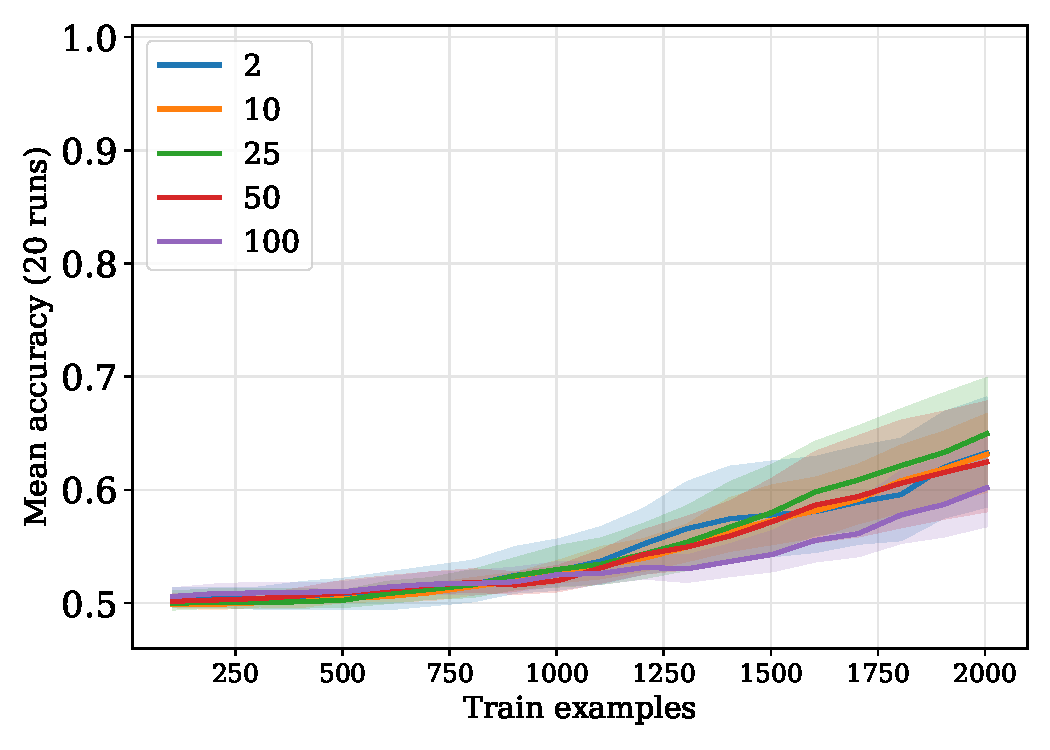
\includegraphics[width=1\textwidth]{../fig/equality-train_size-embed_dim-hidden_dim=2.pdf}
    \caption{Hidden dimensionality 2.}
  \end{subfigure}
  \hfill
  \begin{subfigure}{0.45\linewidth}
    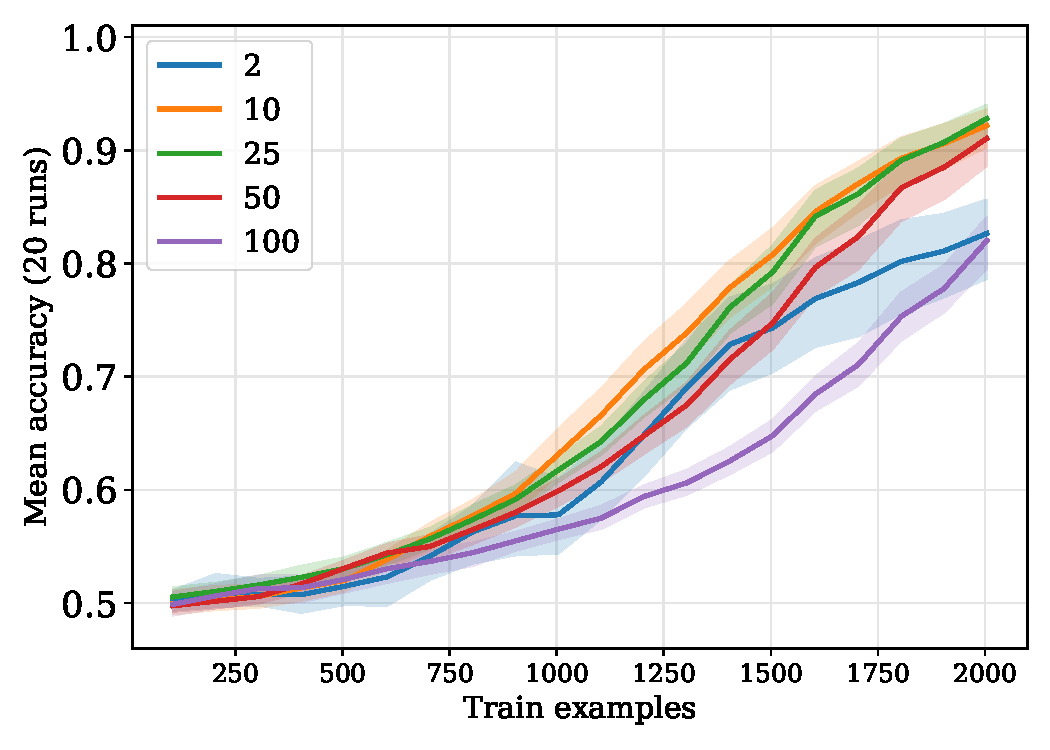
\includegraphics[width=1\textwidth]{../fig/equality-train_size-embed_dim-hidden_dim=10.pdf}
    \caption{Hidden dimensionality 10.}
  \end{subfigure}

  \vspace{24pt}

  \begin{subfigure}{0.45\linewidth}
    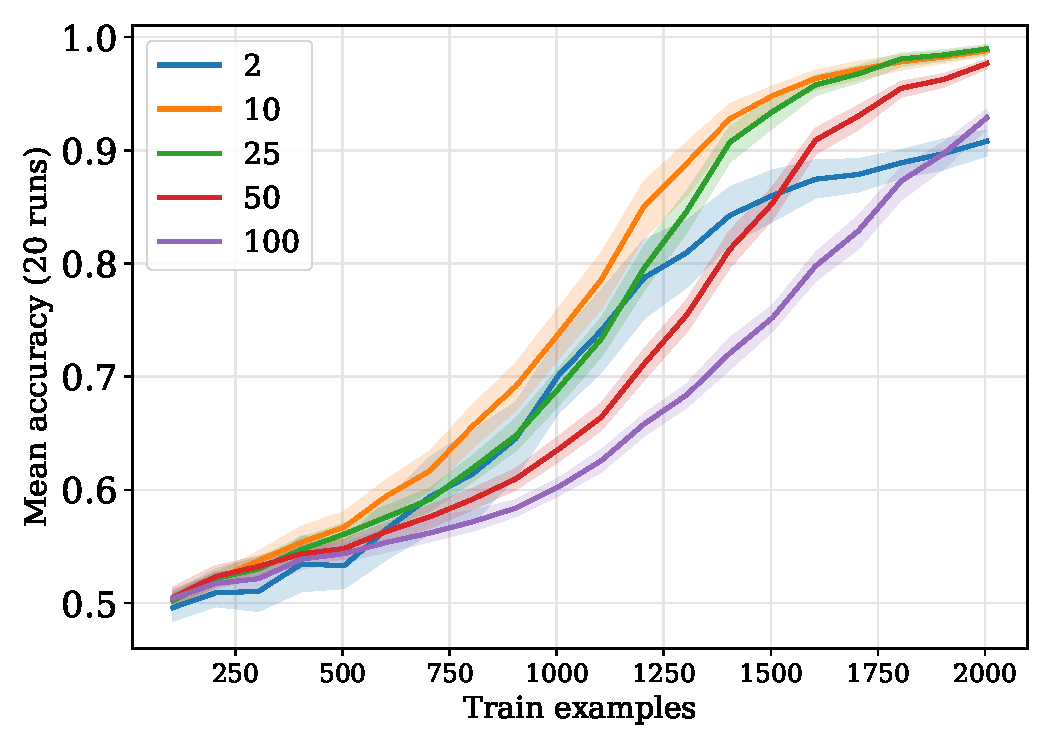
\includegraphics[width=1\textwidth]{../fig/equality-train_size-embed_dim-hidden_dim=25.pdf}
    \caption{Hidden dimensionality 25.}
  \end{subfigure}
  \hfill
  \begin{subfigure}{0.45\linewidth}
    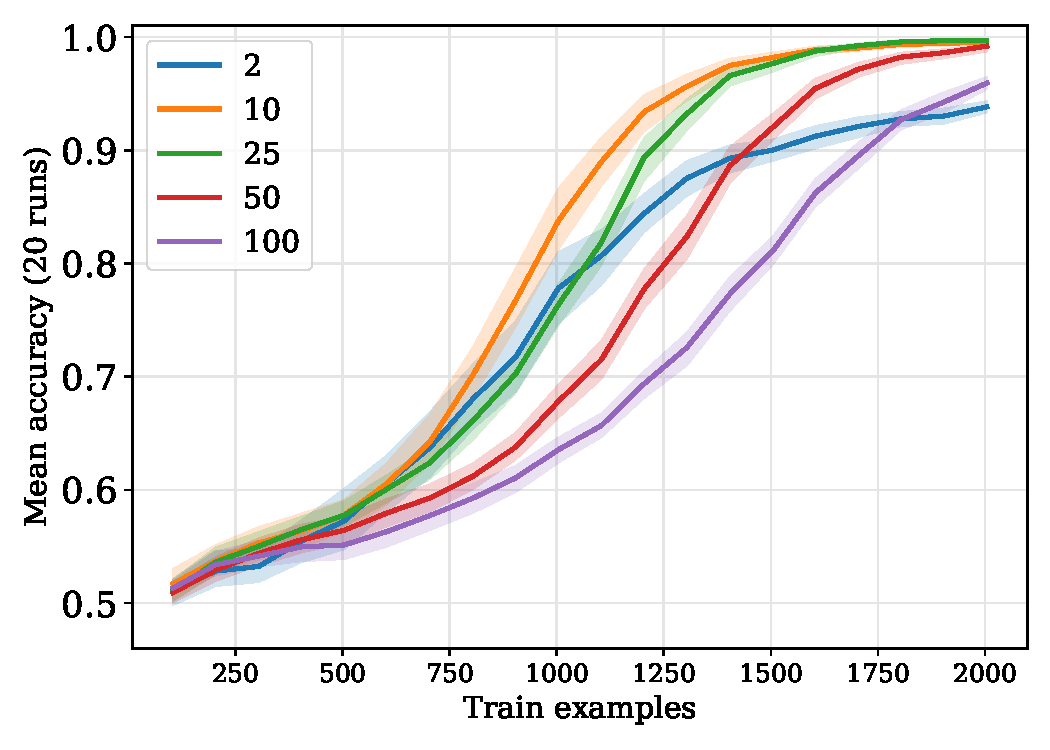
\includegraphics[width=1\textwidth]{../fig/equality-train_size-embed_dim-hidden_dim=50.pdf}
    \caption{Hidden dimensionality 50.}
  \end{subfigure}

  \vspace{24pt}

  \begin{subfigure}{0.45\linewidth}
    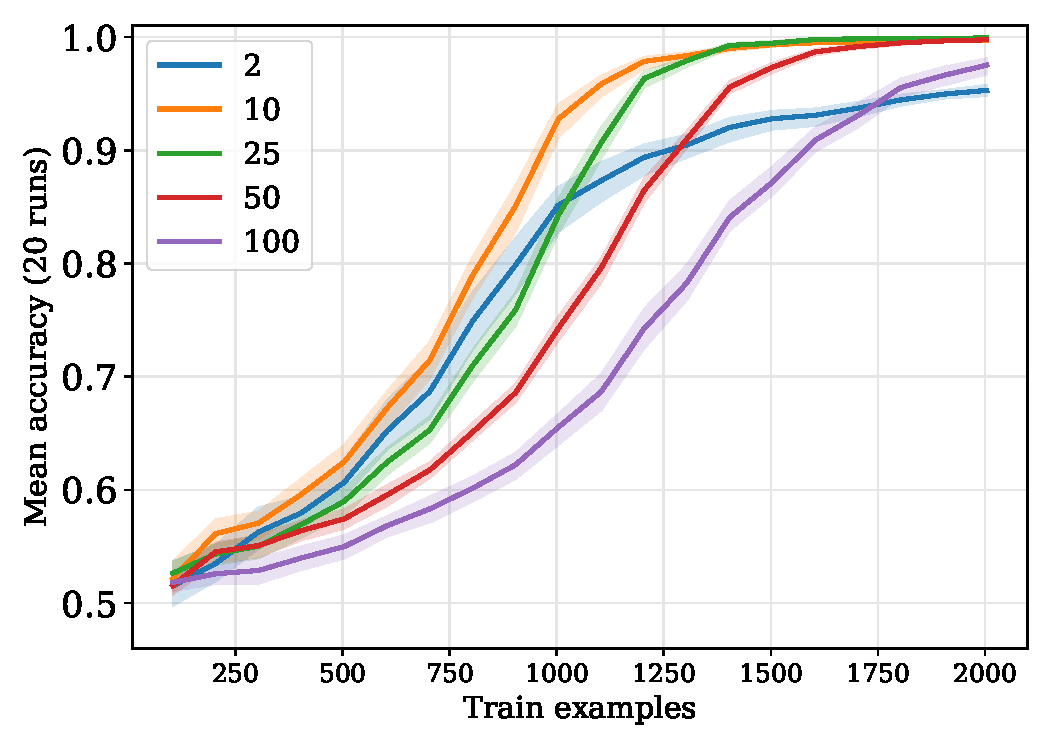
\includegraphics[width=1\textwidth]{../fig/equality-train_size-embed_dim-hidden_dim=100.pdf}
    \caption{Hidden dimensionality 100.}
    \label{fig:model1-rep}
  \end{subfigure}
  \caption{Results for Model 1 for basic same--different.}
  \label{fig:model1}
\end{figure}


\newpage


\subsection{Model 2 for sequential same--different}

\Figref{fig:model2} explores a wider range of hidden dimensionalities for Model~2 applied to the sequential ABA task. As in the paper, the lines correspond to different embedding dimensionalities. The full training set is presented to the model in multiple epochs. \Figref{fig:model2-rep} is repeated from \figref{fig:fuzzy-lm-pretrain-results}.

\begin{figure}[H]
  \centering

  \begin{subfigure}{0.45\linewidth}
    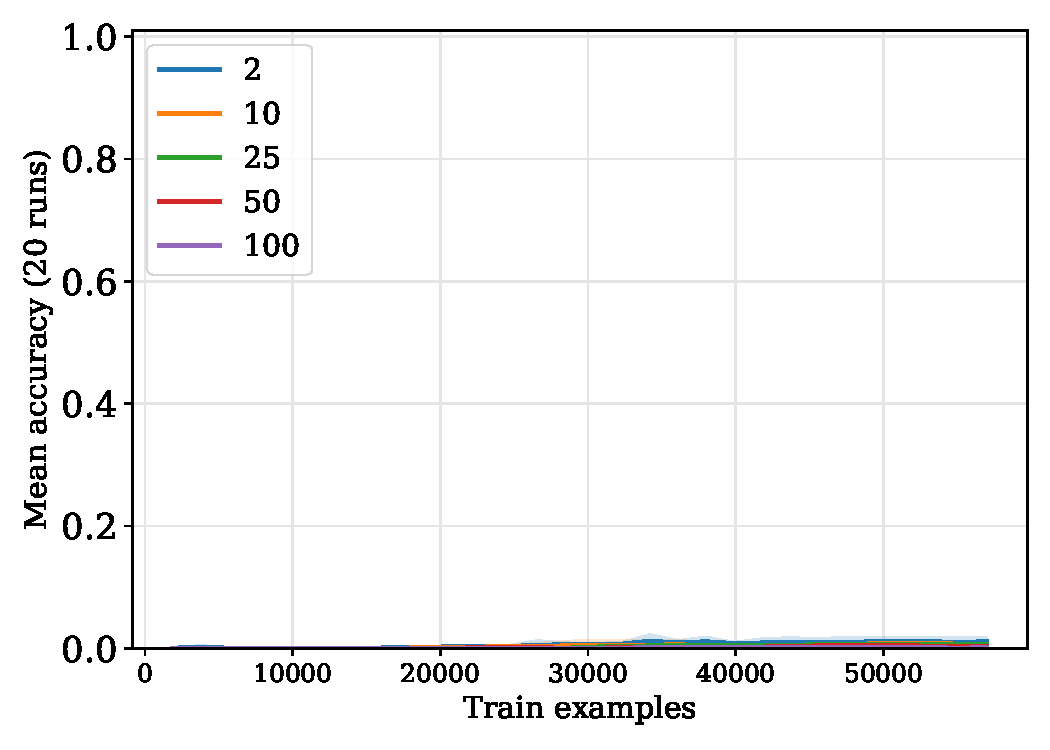
\includegraphics[width=1\textwidth]{../fig/fuzzy-lm-vocab20-pretrain-3tasks-train_size-embed_dim-hidden_dim=2.pdf}
    \caption{Hidden dimensionality 2.}
  \end{subfigure}
  \hfill
  \begin{subfigure}{0.45\linewidth}
    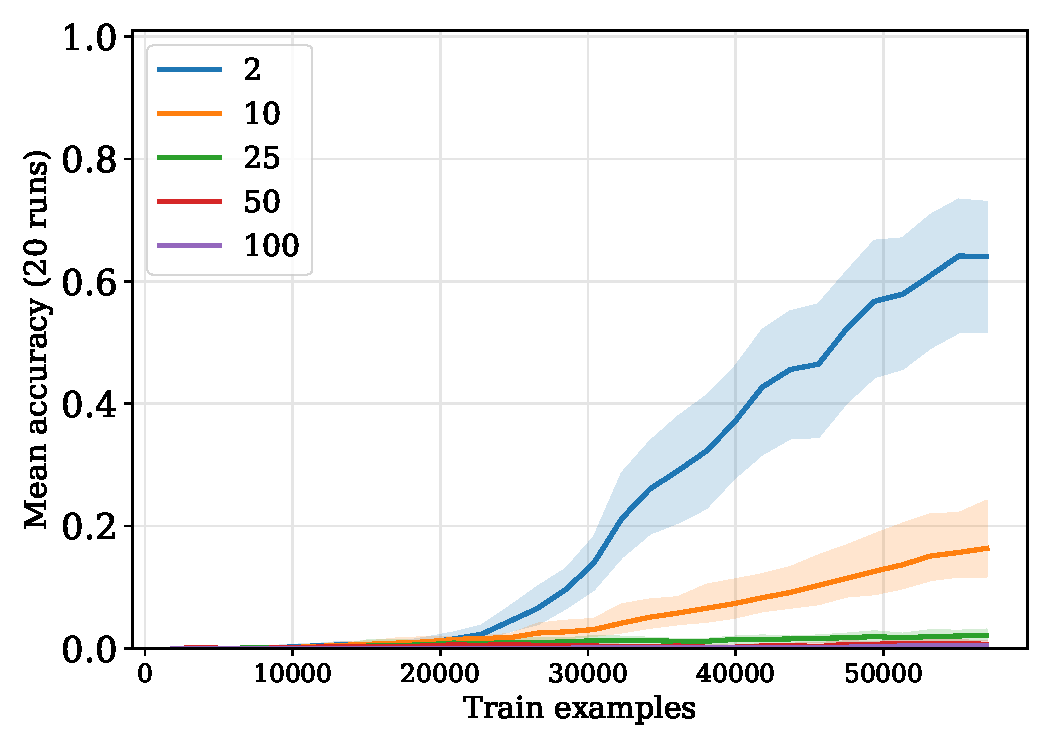
\includegraphics[width=1\textwidth]{../fig/fuzzy-lm-vocab20-pretrain-3tasks-train_size-embed_dim-hidden_dim=10.pdf}
    \caption{Hidden dimensionality 10.}
  \end{subfigure}

  \vspace{24pt}

  \begin{subfigure}{0.45\linewidth}
    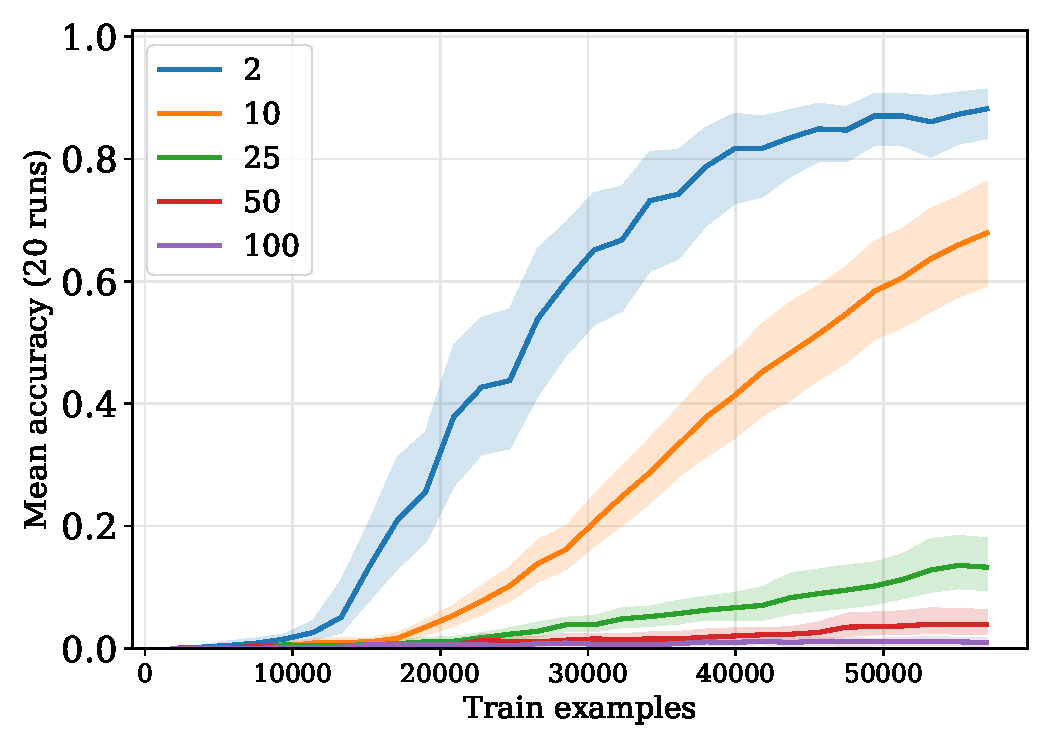
\includegraphics[width=1\textwidth]{../fig/fuzzy-lm-vocab20-pretrain-3tasks-train_size-embed_dim-hidden_dim=25.pdf}
    \caption{Hidden dimensionality 25.}
  \end{subfigure}
  \hfill
  \begin{subfigure}{0.45\linewidth}
    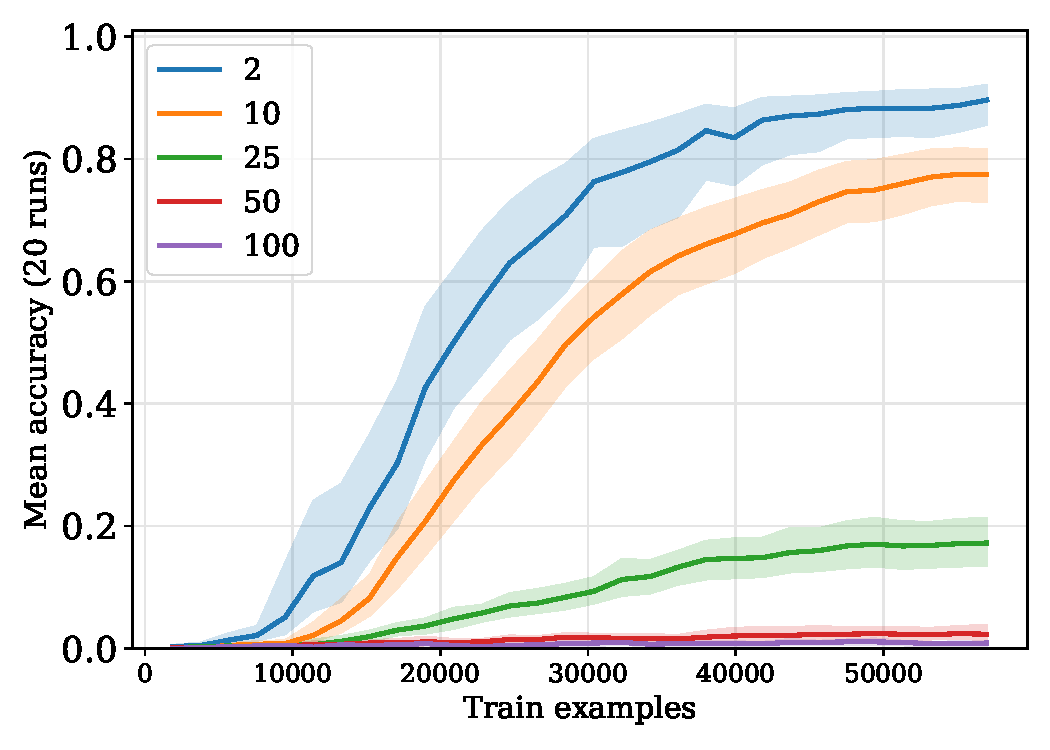
\includegraphics[width=1\textwidth]{../fig/fuzzy-lm-vocab20-pretrain-3tasks-train_size-embed_dim-hidden_dim=50.pdf}
    \caption{Hidden dimensionality 50.}
  \end{subfigure}

  \vspace{24pt}

  \begin{subfigure}{0.45\linewidth}
    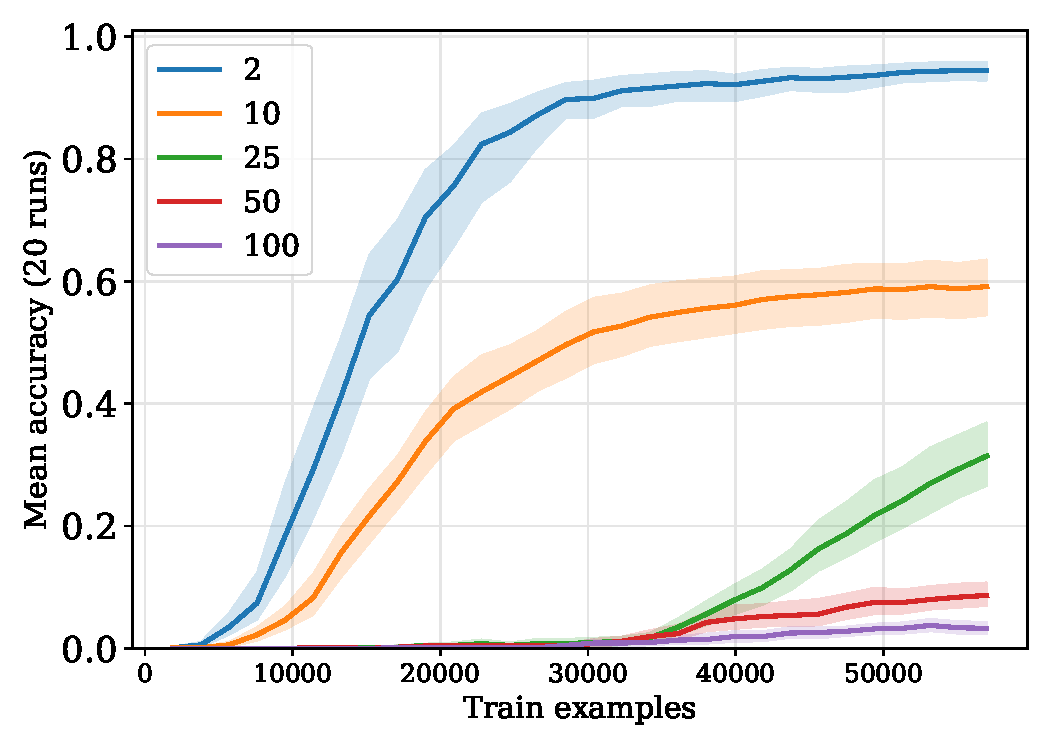
\includegraphics[width=1\textwidth]{../fig/fuzzy-lm-vocab20-pretrain-3tasks-train_size-embed_dim-hidden_dim=100.pdf}
    \caption{Hidden dimensionality 100.}
    \label{fig:model2-rep}
  \end{subfigure}

  \caption{Results for Model 2 for basic same--different, with a vocabulary size of 20.}
  \label{fig:model2}
\end{figure}


\newpage


\subsection{Model 1 for hierarchical same--different}\label{app:model1-premack}

\Figref{fig:model1:premack} shows the results of applying the model in \dasheg{eq:x2h-supp}{eq:h2y-supp} to the hierarchical same--different task. The only change from that model is that the inputs have dimensionality $4m$, since the four distinct representations in task inputs are simply concatenated.


\begin{figure}[H]
  \centering

  \begin{subfigure}{0.45\linewidth}
    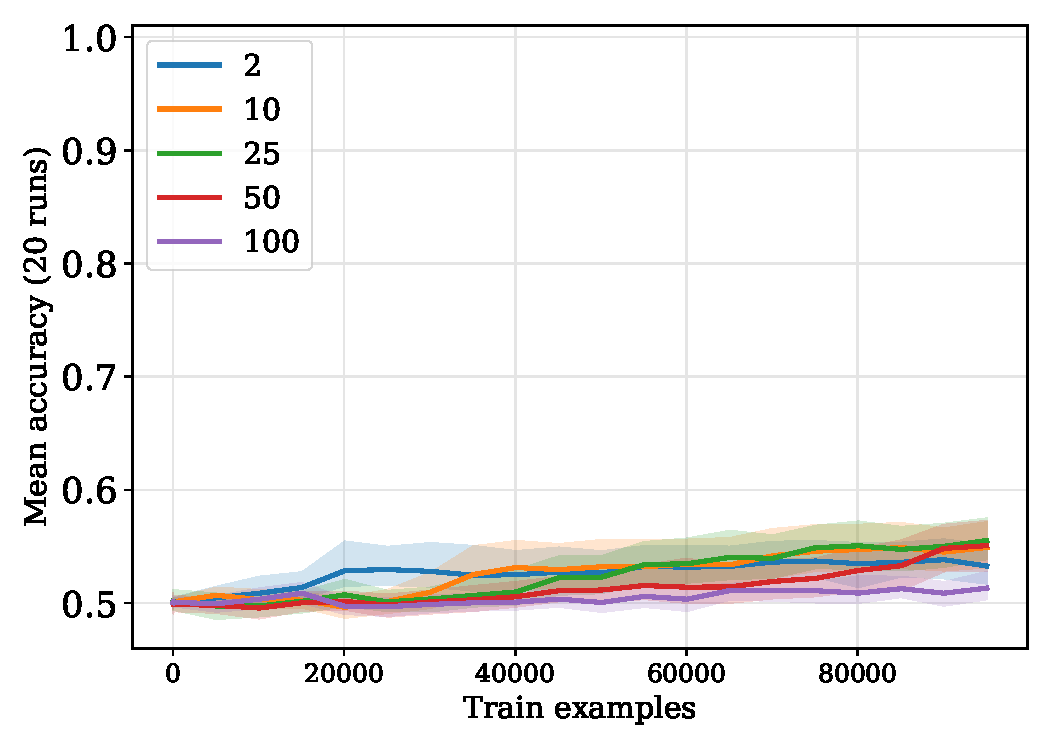
\includegraphics[width=1\textwidth]{../fig/flatpremack-h1-train_size-embed_dim-hidden_dim=2.pdf}
    \caption{Hidden dimensionality 2.}
  \end{subfigure}
  \hfill
  \begin{subfigure}{0.45\linewidth}
    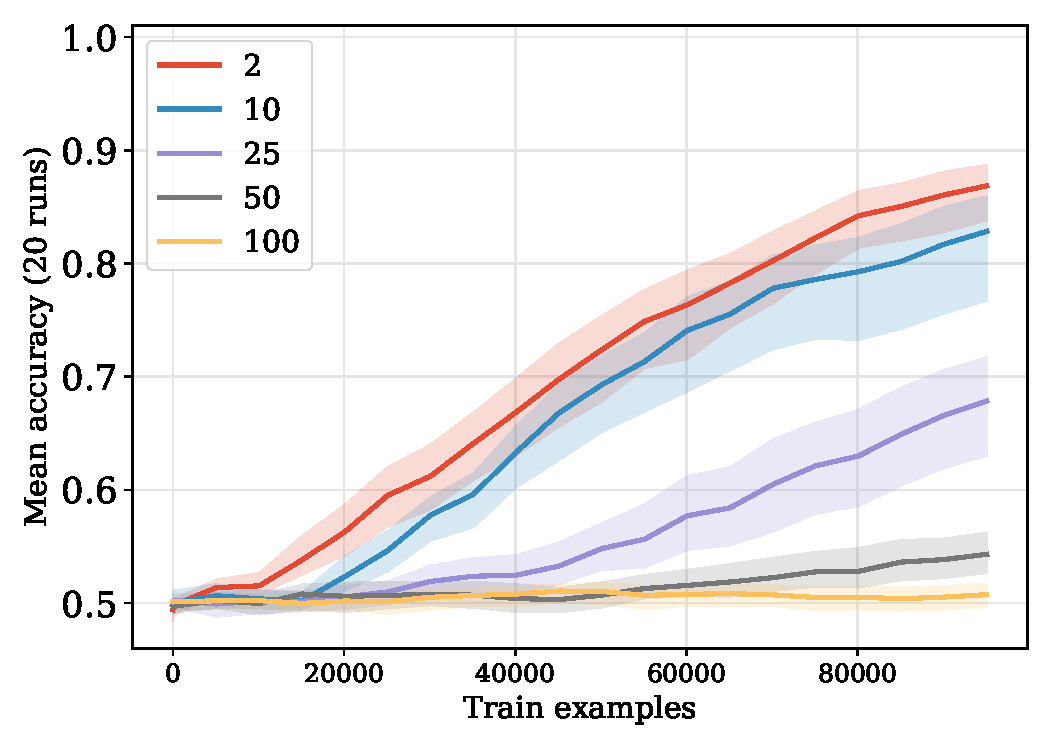
\includegraphics[width=1\textwidth]{../fig/flatpremack-h1-train_size-embed_dim-hidden_dim=10.pdf}
    \caption{Hidden dimensionality 10.}
  \end{subfigure}

  \vspace{24pt}

  \begin{subfigure}{0.45\linewidth}
    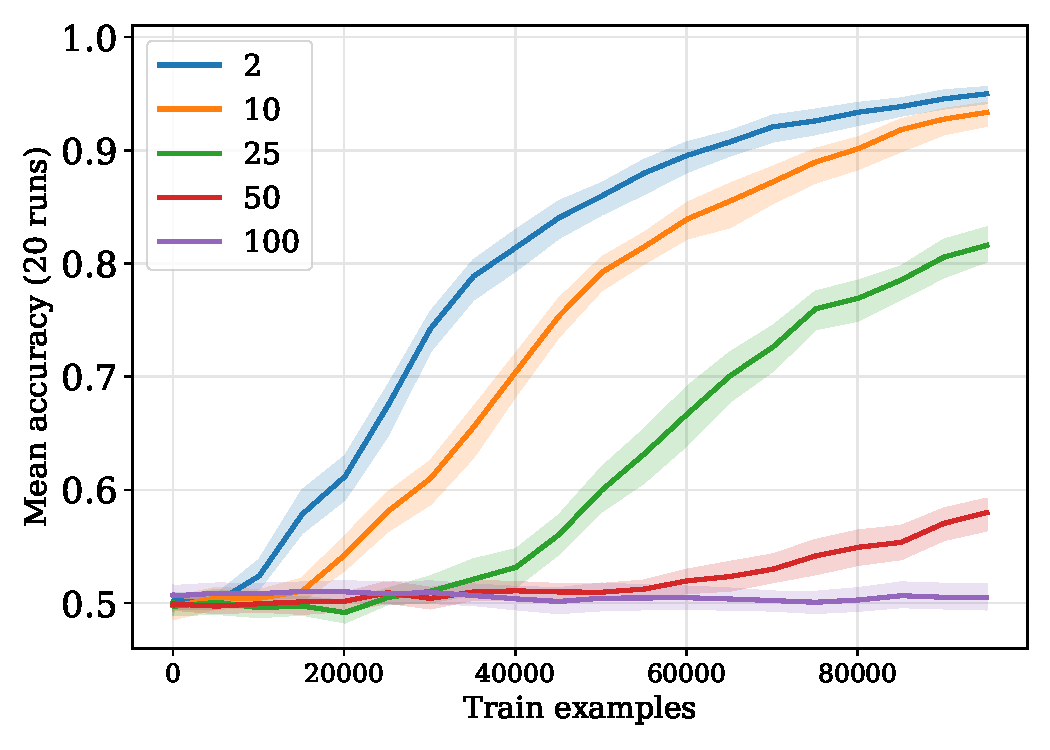
\includegraphics[width=1\textwidth]{../fig/flatpremack-h1-train_size-embed_dim-hidden_dim=25.pdf}
    \caption{Hidden dimensionality 25.}
  \end{subfigure}
  \hfill
  \begin{subfigure}{0.45\linewidth}
    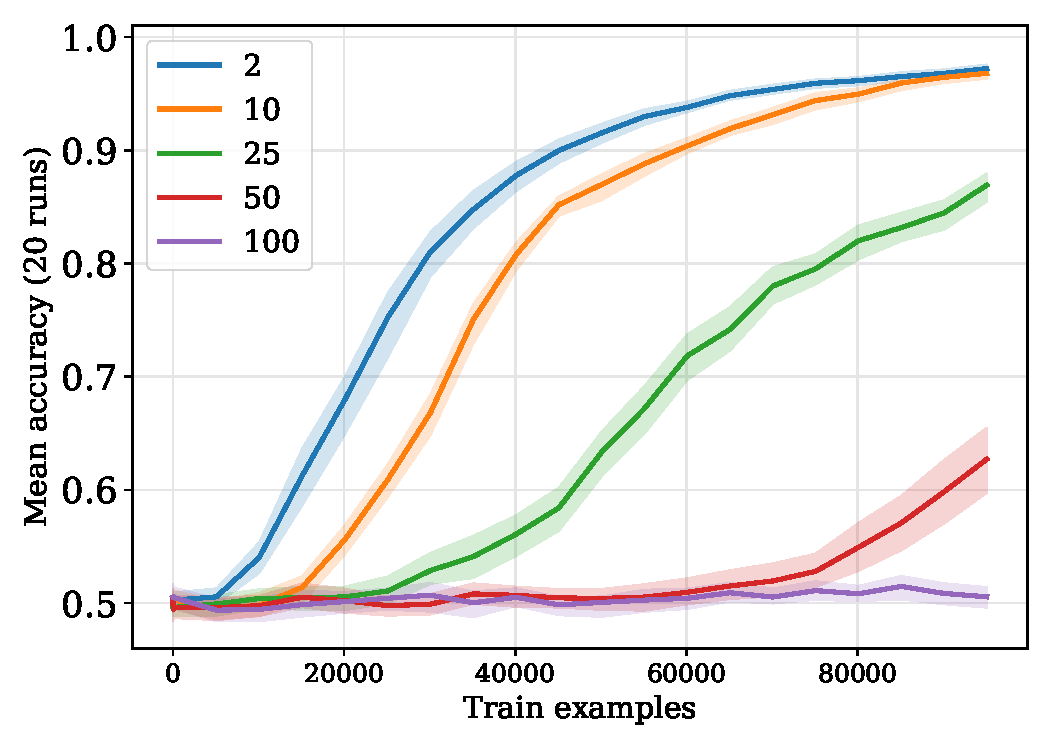
\includegraphics[width=1\textwidth]{../fig/flatpremack-h1-train_size-embed_dim-hidden_dim=50.pdf}
    \caption{Hidden dimensionality 50.}
  \end{subfigure}

  \vspace{24pt}

  \begin{subfigure}{0.45\linewidth}
    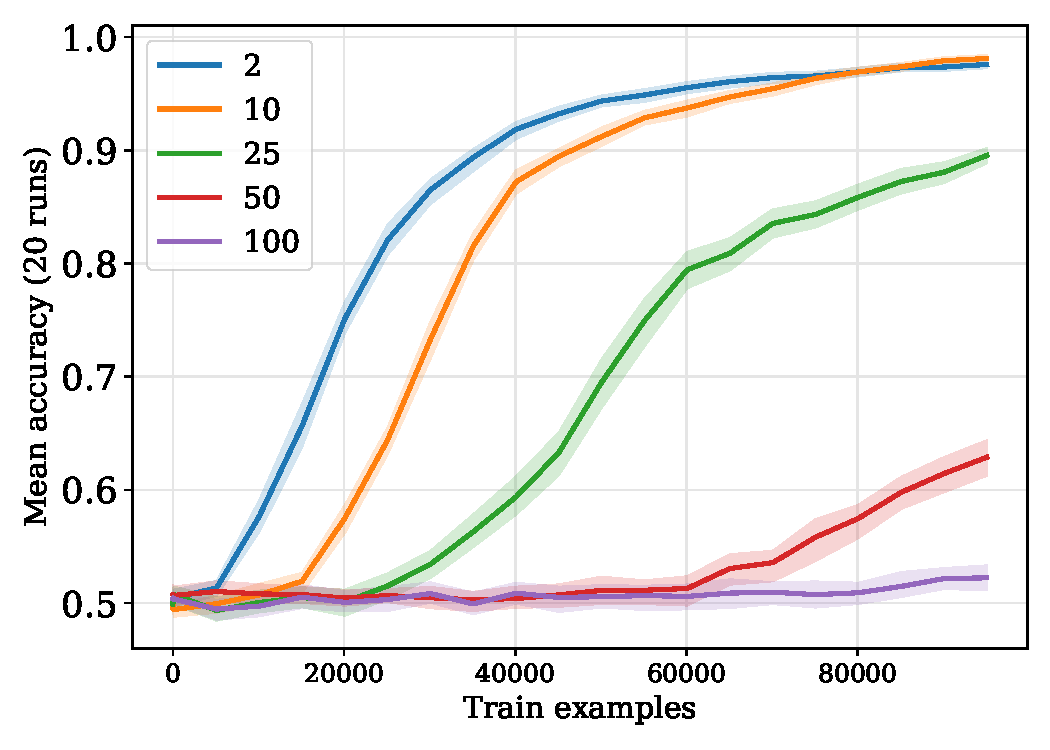
\includegraphics[width=1\textwidth]{../fig/flatpremack-h1-train_size-embed_dim-hidden_dim=100.pdf}
    \caption{Hidden dimensionality 100.}
  \end{subfigure}
  \caption{Results for Model 1 applied to the hierarchical same--different task.}
  \label{fig:model1:premack}
\end{figure}


\newpage


\subsection{Model 3a for hierarchical same--different}

\Figref{fig:model3a} shows the results of applying the model in \dasheg{eq:x2h1-supp}{eq:h2y2-supp} to the hierarchical same--different task. \Figref{fig:model3a-rep} is repeated from \figref{fig:premack-h2-flat-results}.

\begin{figure}[H]
  \centering

  \begin{subfigure}{0.45\linewidth}
    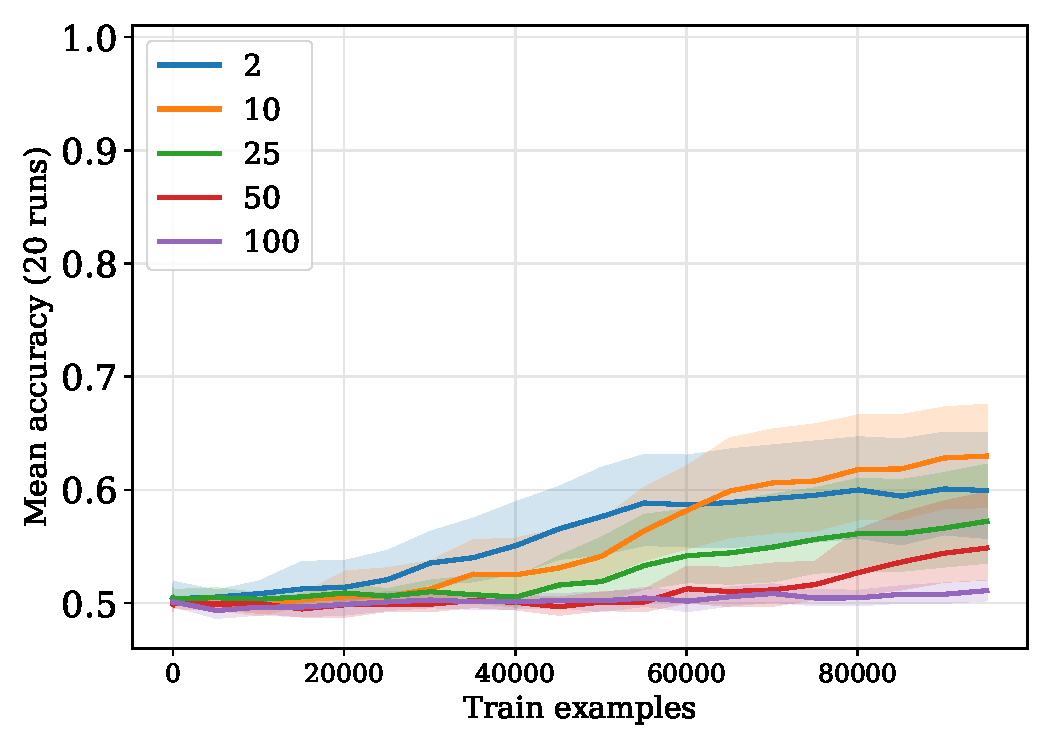
\includegraphics[width=1\textwidth]{../fig/flatpremack-h2-train_size-embed_dim-hidden_dim=2.pdf}
    \caption{Hidden dimensionality 2.}
  \end{subfigure}
  \hfill
  \begin{subfigure}{0.45\linewidth}
    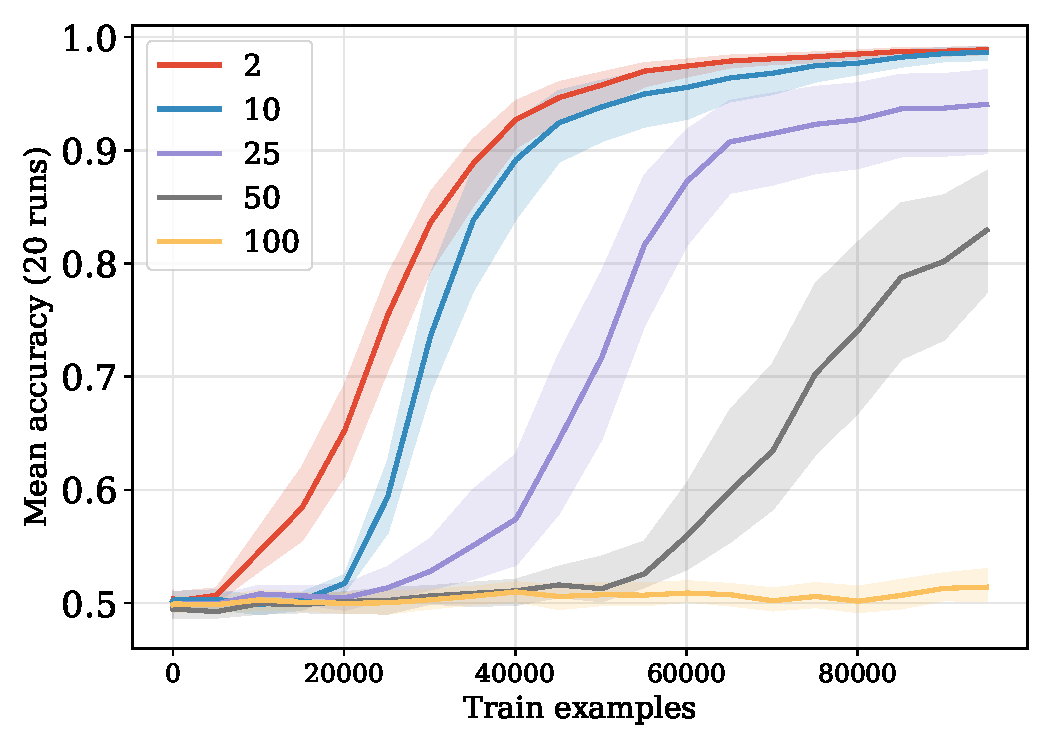
\includegraphics[width=1\textwidth]{../fig/flatpremack-h2-train_size-embed_dim-hidden_dim=10.pdf}
    \caption{Hidden dimensionality 10.}
  \end{subfigure}

  \vspace{24pt}

  \begin{subfigure}{0.45\linewidth}
    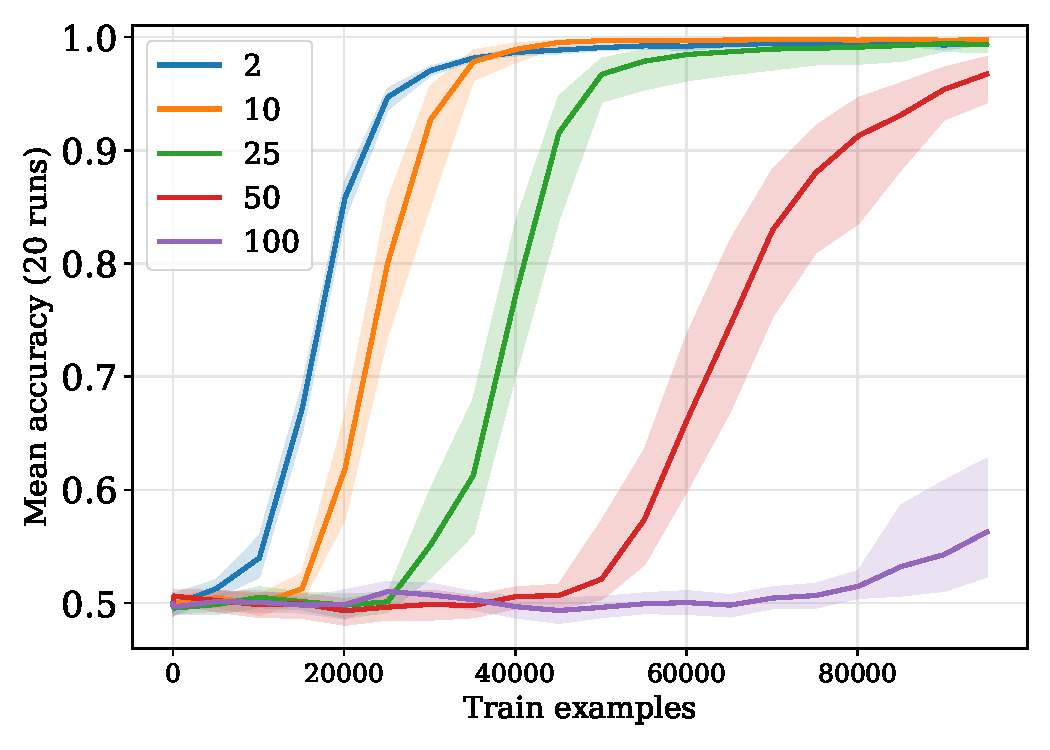
\includegraphics[width=1\textwidth]{../fig/flatpremack-h2-train_size-embed_dim-hidden_dim=25.pdf}
    \caption{Hidden dimensionality 25.}
  \end{subfigure}
  \hfill
  \begin{subfigure}{0.45\linewidth}
    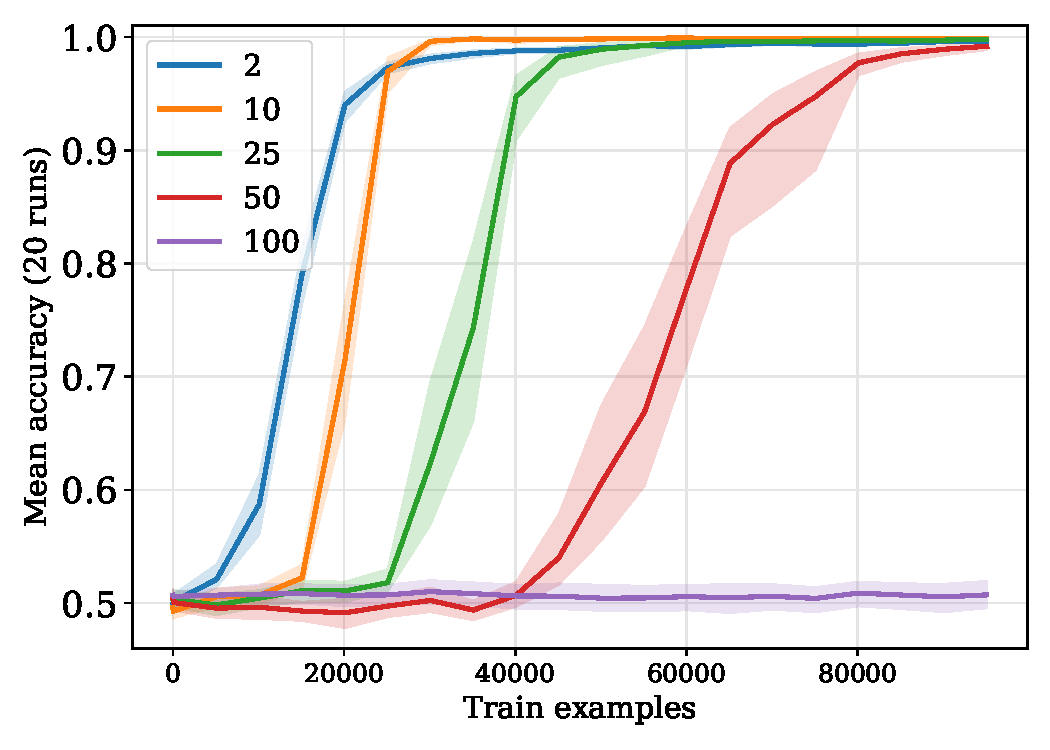
\includegraphics[width=1\textwidth]{../fig/flatpremack-h2-train_size-embed_dim-hidden_dim=50.pdf}
    \caption{Hidden dimensionality 50.}
  \end{subfigure}

  \vspace{24pt}

  \begin{subfigure}{0.45\linewidth}
    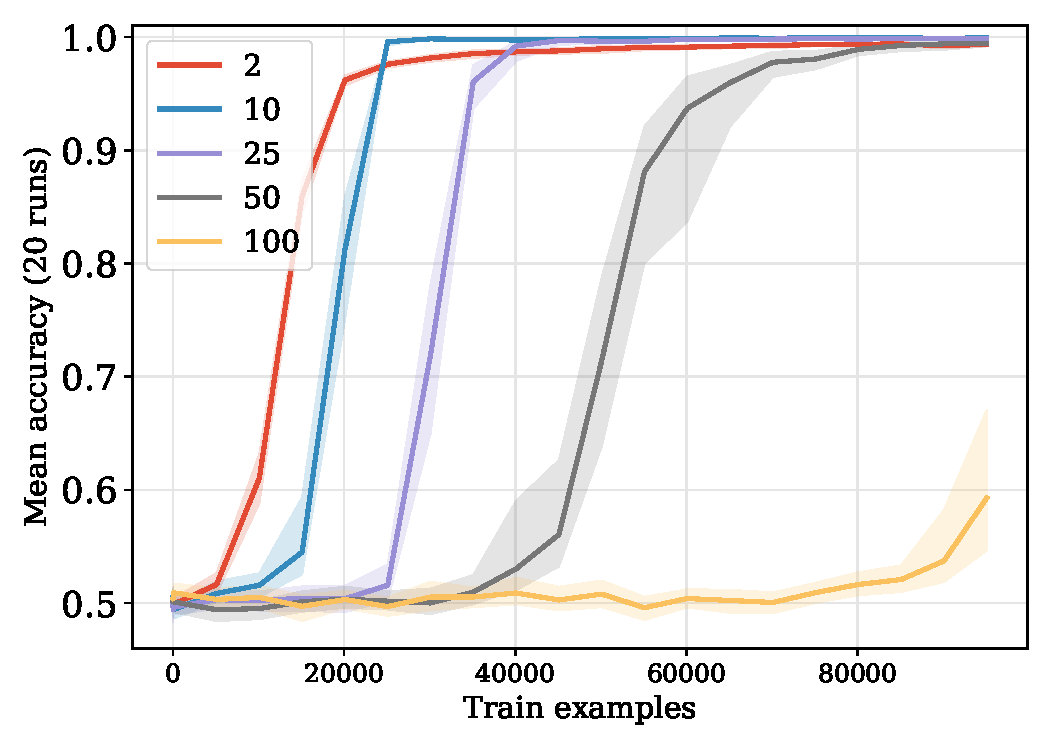
\includegraphics[width=1\textwidth]{../fig/flatpremack-h2-train_size-embed_dim-hidden_dim=100.pdf}
    \caption{Hidden dimensionality 100.}
    \label{fig:model3a-rep}
  \end{subfigure}
  \caption{Results for Model 3a applied to the hierarchical same--different task.}
  \label{fig:model3a}
\end{figure}

\newpage

\subsection{Pretraining input representations and equality parameters}\label{app:double-pretrain}

In \secref{sec:modular}, we showed that pretraining an entire basic equality network led to faster learning in the hierarchical same--different task. This kind of network pretraining can be combined with the input-level pretrained we explored elsewhere in the paper (details in \appref{app:pretraining}). \Figref{fig:double-pretrain} reports initial experiments for this combination of pretraining regimes. Although the results are not better than the ones we report in the paper, this still seems like a promising idea, though one for which optimal solutions might be hard to find.

\begin{figure}[H]
  \centering
  \includegraphics[width=0.48\textwidth]{../fig/input-as-output-pretrain-compare-train_size-pretrained-embed_dim=None.pdf}
  \caption{Results for the hierarchical same--different task for a model in which both the input representations and the basic equality network are pretrained. The `no pretrain' model is the best one from \figref{fig:premack-pretraining-results} (25-dimensional embeddings, 100-dimensional hidden representations). The input-pretrained models use this same configuration.}
  \label{fig:double-pretrain}
\end{figure}

\end{document}


\end{document}
}